\begin{section}{Introduction}
  Solitons and instantons are particular solutions which arise in
  non-linear field theories. An instanton is a solution of the
  euclidian equations of motions which is localized in space
  and time, whereas solitons are stable solutions of the field
  equations with an energy density localized in space.
  
  The instanton is an important element of many calculations in field
  theories. As a simple example, instantons can be used to compute the
  semiclassical transition amplitude between two states:
  \begin{align*}
    \left\langle x_f\middle|e^{-HT/\hbar}\middle|x_i\right\rangle = \int \mathcal D[x]e^{-S/\hbar} = \sqrt{\frac{\omega}{\pi\hbar}}e^{-\omega T/2}\frac{1}{2}\left[e^{ke^{-S_0\hbar}T}\mp e^{-ke^{-S_0\hbar}T}\right]
  \end{align*}
  where $x_f$ and $x_i$ are two vacua, or false vacua, and $S_0$ the
  classical action of the instanton. An extensive discussion on the
  use of instanton is provided by S. Coleman~\cite{col}. Tunnelling
  probabilities may also be obtained.
  
  The situations where the solution to the field equation can be
  expressed in terms of elementary function are exceptional, and arise
  only in the simplest theories. From this point of view, obtaining
  the analytic continuation is not a trivial question.

  In this project, we will develop a framework to compute numerically
  this analytic continuation, provided that a numerical solution of
  the field equations is already available.
  
  We will first check the features and the properties of the procedure
  on a set of test cases, for which solutions are already known. We will
  eventually compute the numerical analytic continuation of the 't
  Hooft--Polyakov monopole in the Georgi--Glashow model, as well as a
  vortex in a $(2+1)$ dimensional Yang-Mills theory with $U(1)$ gauge
  symmetry.

  %Here we need to introduce the context of this work, and explain why
  %it is interesting to find an answer to what we have done.  In
  %particular, it happens that the static solutions of some given
  %theories may be easily expressed in closed form, or integrated
  %numerically. For the same theories, it may not be as easy to find
  %instantons solution for diverse reasons. I need here some citation
  %to give an example of someone using the instantons without knowing
  %it.
  
  %In the general case, the instanton solution is related to the
  %soliton by a change of variable, adding to the radial coordinate an
  %imaginary component, and eventually evaluate the solution on the
  %imaginary axis. The Cauchy theorem guarantees that the integral over
  %fixed boundary path is the same, provided that they belong to the
  %same homotopy class.

  %Instantons are useful to compute transitions amplitudes from
  %different set of states. They can also be useful for semi-classical
  %approximations.\cite{col}

  %Hence the wick rotation is valid as long as the deformation of the
  %path do not cross any singularity.

  %As a numerous of studies rely on the fact that the Wick rotation is
  %valid, it is interesting to convince ourselves that this is indeed
  %the case, using numerical arguments in our case.
\end{section}
\begin{section}{Numerical Scheme}\label{sec:numericalscheme}
  In this section, we develop the framework which will allow us to
  compute numerically the analytic continuation of an arbitrary
  function. Let
  \begin{align}
    \vec f: x\in I\subset\mathbb{R}\mapsto \vec f(x)\in \mathbb{R}^n
  \end{align}
  be a real-valued function, defined by a set of $n$ differential equations
  \begin{align}
    \frac{\mathrm{d}\vec f}{\mathrm{d}x} = \vec F(\vec f(x),x)\label{eq:diffcp}
  \end{align}
  with $n$ initial or boundary conditions which define univocally
  $\vec f$. Then it is possible, using the Cauchy-Riemann equations to
  define a new set of differential equations with initial values,
  which describe the continuation of the function $f$ to the complex
  plane.

  We now assume that the coordinate $x$ is an element of $\mathbb{C}$:
  $x\to z=x+iy$, as well as the function $\vec f$ itself:
  \begin{align}
    \vec f(x)\to \vec f(z)=\vec f_{R}(z)+i\vec f_{I}(z)
  \end{align}
  with $f_{R}$ and $f_{I}$ being the real and imaginary parts of $\vec
  f$. Derivative with respect to $x$ must be changed to:
  \begin{align}
    \frac{\mathrm{d}\vec f}{\mathrm d x} \to \frac{\mathrm{d}\vec f}{\mathrm d z} \equiv \partial_x f_R(x+iy)+i\partial_x f_I(x+iy),
  \end{align}
  and the right hand side of (\ref{eq:diffcp}) is completed by an imaginary part as well:
  \begin{align}
    \vec F(\vec f(x),x) \to \vec F_R(\vec f(z),z)+i\vec F_I(\vec f(z),z).
  \end{align}
  The new system now reads:
  \begin{align}
    &\partial_x f_R(x+iy)+i\partial_x f_I(x+iy) = \vec F_R(\vec f(z),z)+i\vec F_I(\vec f(z),z),\\
    \Rightarrow &\left\{
    \begin{aligned}
      \partial_x f_R(x+iy) = \vec F_R(\vec f(z),z),\\
      \partial_x f_I(x+iy) = \vec F_I(\vec f(z),z).
    \end{aligned}
    \right.\label{eq:cp_before_cr}
  \end{align}
  Assuming that $f$ is analytic, the Cauchy-Riemann equations:
  \begin{align}\label{eq:cr}
    \left\{
    \begin{aligned}
      &\partial_x f_{R} = \partial_{y} f_{I},\\
      &\partial_x f_{R} = -\partial_{x} f_{I},
    \end{aligned}
    \right.
  \end{align}
  provide a relationship between the derivative of the real and
  imaginary parts.  These equation allow to rewrite the system
  (\ref{eq:cp_before_cr}) in terms of the partial derivatives with
  respect to the imaginary coordinate:
  %This relation is the key which
  %makes the difference between a system of partial differential
  %equations, and the problem of analytic continuation.  The system of
  %equations (\ref{eq:cp_before_cr}) can therefore be written in terms
  %of the derivatives with respect to a unique coordinates:
  \begin{align}
    \begin{aligned}
      &\partial_y f_I(x+iy) = \vec F_R(\vec f(z),z),\\
      &-\partial_y f_R(x+iy) = \vec F_I(\vec f(z),z).
    \end{aligned}\label{eq:cp}
  \end{align}
  
  For $f(z)$ to be an analytic continuation of $f(x)$, both functions
  must coincide on the intersection of their domain of definitions,
  that is, on the real axis:
  \begin{align}
    &f_R(x+i0)+if_I(x+i0) = f(x),\quad \forall x,\\
    \Rightarrow 
    &\left\{
    \begin{aligned}
      &f_R(x+i0) = f(x)\\
      &f_I(x+i0) = 0
    \end{aligned}
    \right.,\quad \forall x.
  \end{align}  
  From this point, we may integrate numerically the system
  (\ref{eq:cp}) along $y\in [0,\pm\infty)$ to obtain $f(z)$.
    
  But this procedure is not sufficient for the following
  reasons. First of all, it may happens that the function $f(x)$ is
  only defined or known on a subset of the real line $I\subset
  \mathbb{R}$. In this case, our procedure would only allow us to find
  its analytic continuation on a subset of the complex plane
  $\{z=x+iy\ |\ x\in I\}$. Secondly, it may also happens that the
  function $f$ is not defined or analytic on a set of points $\{z_1
  \equiv x_1+iy_1, z_2 \equiv x_2+iy_2, \dots\}$ away from the real
  axis. In this case, we can only find a numerical solution for the
  points $\{z=x_i+iy\ |\ y<y_i\}$, and the solution cannot be computed
  beyond these points.
  %the numerical scheme would not be valid in the
  %vicinity of such points, and one would not be able to find the
  %function beyond these points: $\{z=x_i+iy | y\geq y_i\},\ \forall
  %i$.
  In practice, we cannot even come arbitrarily close to these
  point, as the numerical scheme becomes unstable.

  We note that the set of points which are not reachable are related
  to the choice of coordinates to represent the complex
  numbers. Hence, changing the coordinates system would also change
  the set of points which is out of reach. Considering different sets
  of coordinates would eventually allow us to find the function
  everywhere.
    
  \begin{subsection}{Polar coordinates}
    The typical situation that may arise is the following. A function
    $f$ is defined $\forall x\in\mathbb{R}_+-\{0\}$, and we are
    interested in its analytic continuation on the imaginary axis.
    %In the particular
    %problem we will encounter, the function to continue will usually
    %only be defined on the real half-line $[0,\infty)$, and we will be
    %interested on the values of the function either on the real
    %half-plane $\{z=x+iy\ |\ x\geq 0\}$, including the imaginary
    %axis, or simply everywhere.
    Choosing a polar coordinate system
    is therefore convenient, since it would be sufficient to
    integrate along the polar angle $\theta\in[0,\pm\pi/2]$.  Let's
    define such a coordinate system by:
    \begin{align}
      z = x(r,\theta) +iy(r,\theta),\text{ where } \left\{
      \begin{aligned}
        x = r\cos(\theta)\\
        y = r\sin(\theta)          
      \end{aligned}
      \right.
    \end{align}
    and the function $f$ in terms of these coordinates:
    \begin{align}
      f(z) = f(x(r,\theta)+iy(r,\theta)) \equiv f(r,\theta).
    \end{align}
    And since we need to integrate the function along $\theta$, we
    need to find the corresponding Cauchy problem for the real and
    imaginary parts of $f(r,\theta)$.
      
      Using the chain rule, we have:
      \begin{align}
        &\frac{\partial f_{R,I}}{\partial \theta}(r,\theta) = \frac{\partial f_{R,I}}{\partial x}(x(r,\theta)+iy(r,\theta))\frac{\partial x}{\partial \theta}(r,\theta)\\
        &\hphantom{\frac{\partial f_{R,I}}{\partial \theta}(r,\theta) = }+ \frac{\partial f_{R,I}}{\partial y}(x(r,\theta)+iy(r,\theta))\frac{\partial y}{\partial \theta}(r,\theta),\\
        &\Rightarrow \left\{
        \begin{aligned}
          \frac{\partial f_{R}}{\partial \theta}(r,\theta) =& \frac{\partial f_{R}}{\partial x}(x(r,\theta)+iy(r,\theta))\frac{\partial x}{\partial \theta}(r,\theta) \\
          &+ \frac{\partial f_{R}}{\partial y}(x(r,\theta)+iy(r,\theta))\frac{\partial y}{\partial \theta}(r,\theta),\\
          \frac{\partial f_{I}}{\partial \theta}(r,\theta) =& \frac{\partial f_{I}}{\partial x}(x(r,\theta)+iy(r,\theta))\frac{\partial x}{\partial \theta}(r,\theta) \\
          &+ \frac{\partial f_{I}}{\partial y}(x(r,\theta)+iy(r,\theta))\frac{\partial y}{\partial \theta}(r,\theta).
        \end{aligned}
        \right.
      \end{align}

      At this point, we may use the original differential system
      (\ref{eq:cp_before_cr}) and (\ref{eq:cp}) to substitute the
      derivatives of $f$:
      \begin{align}
\left\{
        \begin{aligned}
          \frac{\partial f_{R}}{\partial \theta}(r,\theta) =& F_{R}(f(x(r,\theta)+iy(r,\theta)),z(r,\theta))\frac{\partial x}{\partial \theta}(r,\theta) \\
          &-F_{I}(f(x(r,\theta)+iy(r,\theta)),z(r,\theta))\frac{\partial y}{\partial \theta}(r,\theta),\\
          \frac{\partial f_{I}}{\partial \theta}(r,\theta) =& F_{I}(f(x(r,\theta)+iy(r,\theta)),z(r,\theta))\frac{\partial x}{\partial \theta}(r,\theta) \\
          &+ F_{R}(f(x(r,\theta)+iy(r,\theta)),z(r,\theta))\frac{\partial y}{\partial \theta}(r,\theta),
        \end{aligned}
        \right.
      \end{align}
      which can be expressed in the more compact form:
      \begin{align}
        \begin{bmatrix}
          \partial_\theta f_{R}(r,\theta)\\
          \partial_\theta f_{I}(r,\theta)
        \end{bmatrix}
        = 
        \begin{bmatrix}
          \partial_\theta x(r,\theta) & -\partial_\theta y(r,\theta)\\
          \partial_\theta y(r,\theta) & \partial_\theta x(r,\theta)\\
        \end{bmatrix}\cdot
        \begin{bmatrix}
          F_{R}(f(z(r,\theta)), z(r,\theta))\\
          F_{I}(f(z(r,\theta)), z(r,\theta))
        \end{bmatrix}.
      \end{align}
      This last expression is valid for any change of coordinates,
      since we didn't used any special properties of polar
      coordinates.
      
      Eventually, the polar coordinates leads to the following
      differential system:
      \begin{align}
        \begin{bmatrix}
          \partial_\theta f_{R}(r,\theta)\\
          \partial_\theta f_{I}(r,\theta)
        \end{bmatrix}
        =-r
        \begin{bmatrix}
          \sin(\theta) & \cos(\theta)\\
          -\cos(\theta) &  \sin(\theta)\\
        \end{bmatrix}\cdot
        \begin{bmatrix}
          F_{R}(f(z(r,\theta)), z(r,\theta))\\
          F_{I}(f(z(r,\theta)), z(r,\theta))
        \end{bmatrix}.
      \end{align}
    \end{subsection}
    The initial conditions are given by:
    \begin{align}
      \left\{
      \begin{aligned}
        &f_R(r,\theta=0) = f_R(r+0i) = f(r)\\
        &f_I(r,\theta=0) = f_I(r+0i) = 0
      \end{aligned}
      \right.\quad \forall r>0,
    \end{align}
    where $f(r)$ is the solution of the problem on the real axis.
    %The integration of the function was performed using a standard
    %Runge-Kutta 4 solver, with fixed step size.
  \begin{subsection}{Vortex and Monopole solutions}
    A prior condition to use our procedure to compute the analytic
    continuation of a function to the complex plane is to know the
    function on the real axis. For the vortex and the monopole, this
    requires to solve a system of two non linear differential
    equations with boundary conditions at the origin and infinity.
    %Let's recall the contexts of each theory.  In this section, we
    give a brief descriptions of the theories. A more detailed
    discussion can be found in \cite{rub} and \cite{shn}.
    \begin{subsubsection}{The Vortex in $(2+1)$ dimensions}\label{sec:theory_vortex}
      Let $\mathcal L$ be the Lagrangian of a field theory with $U(1)$
      gauge symmetry in $(2+1)$ dimensions:
      \begin{align}
        \mathcal L = -\frac{1}{4}F^2_{\mu\nu} + (D_\mu\phi)^*(D_\mu\phi)-\frac{\lambda}{2}(\phi^*\phi-v^2)^2.
      \end{align}
      Under the condition of finiteness of the energy functional, the
      most general static spherically symmetric ansatz can be written as:
      \begin{align}
        &A_i(r,\theta) = -\frac{1}{er}\varepsilon_{ij}n_jA(r),\ A_0 = 0,\\
        &\phi(r,\theta) = ve^{i\theta}F(r),
      \end{align}
      with the following asymptotics for the two functions $A$ and $F$:
      \begin{align}
        A(0) = F(0) = 0,\\
        \lim_{r\to\infty}A(r) = \lim_{r\to\infty}F(r) = 1.
      \end{align}
      Substitution of this ansatz into the equations of motions leads
      to the two independent second order differential equations:
      \begin{align}
        -\frac{\mathrm d}{\mathrm d r}\left(\frac{1}{r}\frac{\mathrm d A}{\mathrm d r}\right)-2e^2v^2\frac{F^2(1-A)}{r} = 0,\label{eq:vortex_1}\\
        -\frac{\mathrm d}{\mathrm d r}\left(r\frac{\mathrm d F}{\mathrm d r}\right) + \lambda v^2 r F(F^2-1)+\frac{F(1-A)^2}{r} = 0.\label{eq:vortex_2}
      \end{align}
      There exist no expression of the solution in terms of elementary
      functions for this problem, thus we are forced to use numerical
      tools to find an approximation. The numerical techniques available
      to solve such boundary value problems fall into two main
      categories.
      
      The first uses a finite element method approach to approximate
      the derivatives of the functions, reducing the problem to
      finding zeros of a set of non linear equations.  A
      Newton-Raphson iteration is then used to find a numerical
      solution to the system.
      
      The second category, generally called shooting method, takes
      advantage of all the well-developed techniques available to
      tackle differential initial value problems, by considering the
      the boundary values at one extremity of the interval as a
      function of the boundary values at the other extremity. We then
      need to find the right initial condition such that the solution
      satisfies the both boundary conditions.
      
      This last method fails in a number of situations, including the
      case of the vortex, especially when the equations are highly non
      linear, and tends to develop exponentially growing
      modes. Careful modification of these methods must be considered
      in these situations.
      %There exist many generalisations which address to compensate
      %some of the drawbacks, for example by splitting the integration
      %interval into a set of subintervals.

      For simplicity, a finite elements method have been used to find
      approximations of the vortex and the monopole, and have shown
      fast convergence to the solution, even when the initial point of
      the Newton-Raphson iteration is far from the solution. Details
      of the computations and the equations used are presented for the
      interested reader in appendix \ref{ann:num}.  The code was
      implemented in the C++ language, with the use of the Lapack
      routines for some linear algebra related operations, such as
      matrix inversion.

      \begin{figure}[!ht]
        \begin{center}
          % GNUPLOT: LaTeX picture with Postscript
\begingroup
\scriptsize
  \makeatletter
  \providecommand\color[2][]{%
    \GenericError{(gnuplot) \space\space\space\@spaces}{%
      Package color not loaded in conjunction with
      terminal option `colourtext'%
    }{See the gnuplot documentation for explanation.%
    }{Either use 'blacktext' in gnuplot or load the package
      color.sty in LaTeX.}%
    \renewcommand\color[2][]{}%
  }%
  \providecommand\includegraphics[2][]{%
    \GenericError{(gnuplot) \space\space\space\@spaces}{%
      Package graphicx or graphics not loaded%
    }{See the gnuplot documentation for explanation.%
    }{The gnuplot epslatex terminal needs graphicx.sty or graphics.sty.}%
    \renewcommand\includegraphics[2][]{}%
  }%
  \providecommand\rotatebox[2]{#2}%
  \@ifundefined{ifGPcolor}{%
    \newif\ifGPcolor
    \GPcolortrue
  }{}%
  \@ifundefined{ifGPblacktext}{%
    \newif\ifGPblacktext
    \GPblacktexttrue
  }{}%
  % define a \g@addto@macro without @ in the name:
  \let\gplgaddtomacro\g@addto@macro
  % define empty templates for all commands taking text:
  \gdef\gplbacktext{}%
  \gdef\gplfronttext{}%
  \makeatother
  \ifGPblacktext
    % no textcolor at all
    \def\colorrgb#1{}%
    \def\colorgray#1{}%
  \else
    % gray or color?
    \ifGPcolor
      \def\colorrgb#1{\color[rgb]{#1}}%
      \def\colorgray#1{\color[gray]{#1}}%
      \expandafter\def\csname LTw\endcsname{\color{white}}%
      \expandafter\def\csname LTb\endcsname{\color{black}}%
      \expandafter\def\csname LTa\endcsname{\color{black}}%
      \expandafter\def\csname LT0\endcsname{\color[rgb]{1,0,0}}%
      \expandafter\def\csname LT1\endcsname{\color[rgb]{0,1,0}}%
      \expandafter\def\csname LT2\endcsname{\color[rgb]{0,0,1}}%
      \expandafter\def\csname LT3\endcsname{\color[rgb]{1,0,1}}%
      \expandafter\def\csname LT4\endcsname{\color[rgb]{0,1,1}}%
      \expandafter\def\csname LT5\endcsname{\color[rgb]{1,1,0}}%
      \expandafter\def\csname LT6\endcsname{\color[rgb]{0,0,0}}%
      \expandafter\def\csname LT7\endcsname{\color[rgb]{1,0.3,0}}%
      \expandafter\def\csname LT8\endcsname{\color[rgb]{0.5,0.5,0.5}}%
    \else
      % gray
      \def\colorrgb#1{\color{black}}%
      \def\colorgray#1{\color[gray]{#1}}%
      \expandafter\def\csname LTw\endcsname{\color{white}}%
      \expandafter\def\csname LTb\endcsname{\color{black}}%
      \expandafter\def\csname LTa\endcsname{\color{black}}%
      \expandafter\def\csname LT0\endcsname{\color{black}}%
      \expandafter\def\csname LT1\endcsname{\color{black}}%
      \expandafter\def\csname LT2\endcsname{\color{black}}%
      \expandafter\def\csname LT3\endcsname{\color{black}}%
      \expandafter\def\csname LT4\endcsname{\color{black}}%
      \expandafter\def\csname LT5\endcsname{\color{black}}%
      \expandafter\def\csname LT6\endcsname{\color{black}}%
      \expandafter\def\csname LT7\endcsname{\color{black}}%
      \expandafter\def\csname LT8\endcsname{\color{black}}%
    \fi
  \fi
  \setlength{\unitlength}{0.0500bp}%
  \begin{picture}(6236.00,2834.00)%
    \gplgaddtomacro\gplbacktext{%
      \csname LTb\endcsname%
      \put(946,704){\makebox(0,0)[r]{\strut{} 0}}%
      \put(946,1015){\makebox(0,0)[r]{\strut{} 0.2}}%
      \put(946,1326){\makebox(0,0)[r]{\strut{} 0.4}}%
      \put(946,1637){\makebox(0,0)[r]{\strut{} 0.6}}%
      \put(946,1947){\makebox(0,0)[r]{\strut{} 0.8}}%
      \put(946,2258){\makebox(0,0)[r]{\strut{} 1}}%
      \put(1078,484){\makebox(0,0){\strut{} 0}}%
      \put(2043,484){\makebox(0,0){\strut{} 2}}%
      \put(3009,484){\makebox(0,0){\strut{} 4}}%
      \put(3974,484){\makebox(0,0){\strut{} 6}}%
      \put(4940,484){\makebox(0,0){\strut{} 8}}%
      \put(5905,484){\makebox(0,0){\strut{} 10}}%
      \put(308,1636){\rotatebox{-270}{\makebox(0,0){\strut{}$A(f)$}}}%
      \put(3491,154){\makebox(0,0){\strut{}$r$}}%
    }%
    \gplgaddtomacro\gplfronttext{%
      \csname LTb\endcsname%
      \put(4918,1317){\makebox(0,0)[r]{\strut{}$\lambda=0.5$}}%
      \csname LTb\endcsname%
      \put(4918,1097){\makebox(0,0)[r]{\strut{}$\lambda=1$}}%
      \csname LTb\endcsname%
      \put(4918,877){\makebox(0,0)[r]{\strut{}$\lambda=2$}}%
    }%
    \gplbacktext
    \put(0,0){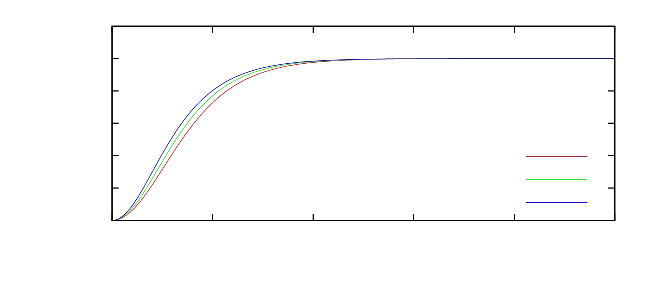
\includegraphics{vortex_func_a}}%
    \gplfronttext
  \end{picture}%
\endgroup

          \caption{\em Profile of the function $A(r)$ for a set of 3
            value for the $\lambda$ coupling constant. A numerical
            approximation of the function is obtained with a
            discretization of the interval $[0,10]$ into $N = 400$
            points. The BPS limit correspond to the green curve.}
          \label{fig:2d_vortex_a}
        \end{center}
      \end{figure}
      
      \begin{figure}[!ht]
        \begin{center}
          % GNUPLOT: LaTeX picture with Postscript
\begingroup
\scriptsize
  \makeatletter
  \providecommand\color[2][]{%
    \GenericError{(gnuplot) \space\space\space\@spaces}{%
      Package color not loaded in conjunction with
      terminal option `colourtext'%
    }{See the gnuplot documentation for explanation.%
    }{Either use 'blacktext' in gnuplot or load the package
      color.sty in LaTeX.}%
    \renewcommand\color[2][]{}%
  }%
  \providecommand\includegraphics[2][]{%
    \GenericError{(gnuplot) \space\space\space\@spaces}{%
      Package graphicx or graphics not loaded%
    }{See the gnuplot documentation for explanation.%
    }{The gnuplot epslatex terminal needs graphicx.sty or graphics.sty.}%
    \renewcommand\includegraphics[2][]{}%
  }%
  \providecommand\rotatebox[2]{#2}%
  \@ifundefined{ifGPcolor}{%
    \newif\ifGPcolor
    \GPcolortrue
  }{}%
  \@ifundefined{ifGPblacktext}{%
    \newif\ifGPblacktext
    \GPblacktexttrue
  }{}%
  % define a \g@addto@macro without @ in the name:
  \let\gplgaddtomacro\g@addto@macro
  % define empty templates for all commands taking text:
  \gdef\gplbacktext{}%
  \gdef\gplfronttext{}%
  \makeatother
  \ifGPblacktext
    % no textcolor at all
    \def\colorrgb#1{}%
    \def\colorgray#1{}%
  \else
    % gray or color?
    \ifGPcolor
      \def\colorrgb#1{\color[rgb]{#1}}%
      \def\colorgray#1{\color[gray]{#1}}%
      \expandafter\def\csname LTw\endcsname{\color{white}}%
      \expandafter\def\csname LTb\endcsname{\color{black}}%
      \expandafter\def\csname LTa\endcsname{\color{black}}%
      \expandafter\def\csname LT0\endcsname{\color[rgb]{1,0,0}}%
      \expandafter\def\csname LT1\endcsname{\color[rgb]{0,1,0}}%
      \expandafter\def\csname LT2\endcsname{\color[rgb]{0,0,1}}%
      \expandafter\def\csname LT3\endcsname{\color[rgb]{1,0,1}}%
      \expandafter\def\csname LT4\endcsname{\color[rgb]{0,1,1}}%
      \expandafter\def\csname LT5\endcsname{\color[rgb]{1,1,0}}%
      \expandafter\def\csname LT6\endcsname{\color[rgb]{0,0,0}}%
      \expandafter\def\csname LT7\endcsname{\color[rgb]{1,0.3,0}}%
      \expandafter\def\csname LT8\endcsname{\color[rgb]{0.5,0.5,0.5}}%
    \else
      % gray
      \def\colorrgb#1{\color{black}}%
      \def\colorgray#1{\color[gray]{#1}}%
      \expandafter\def\csname LTw\endcsname{\color{white}}%
      \expandafter\def\csname LTb\endcsname{\color{black}}%
      \expandafter\def\csname LTa\endcsname{\color{black}}%
      \expandafter\def\csname LT0\endcsname{\color{black}}%
      \expandafter\def\csname LT1\endcsname{\color{black}}%
      \expandafter\def\csname LT2\endcsname{\color{black}}%
      \expandafter\def\csname LT3\endcsname{\color{black}}%
      \expandafter\def\csname LT4\endcsname{\color{black}}%
      \expandafter\def\csname LT5\endcsname{\color{black}}%
      \expandafter\def\csname LT6\endcsname{\color{black}}%
      \expandafter\def\csname LT7\endcsname{\color{black}}%
      \expandafter\def\csname LT8\endcsname{\color{black}}%
    \fi
  \fi
  \setlength{\unitlength}{0.0500bp}%
  \begin{picture}(6236.00,2834.00)%
    \gplgaddtomacro\gplbacktext{%
      \csname LTb\endcsname%
      \put(946,704){\makebox(0,0)[r]{\strut{} 0}}%
      \put(946,1015){\makebox(0,0)[r]{\strut{} 0.2}}%
      \put(946,1326){\makebox(0,0)[r]{\strut{} 0.4}}%
      \put(946,1637){\makebox(0,0)[r]{\strut{} 0.6}}%
      \put(946,1947){\makebox(0,0)[r]{\strut{} 0.8}}%
      \put(946,2258){\makebox(0,0)[r]{\strut{} 1}}%
      \put(1078,484){\makebox(0,0){\strut{} 0}}%
      \put(2043,484){\makebox(0,0){\strut{} 2}}%
      \put(3009,484){\makebox(0,0){\strut{} 4}}%
      \put(3974,484){\makebox(0,0){\strut{} 6}}%
      \put(4940,484){\makebox(0,0){\strut{} 8}}%
      \put(5905,484){\makebox(0,0){\strut{} 10}}%
      \put(308,1636){\rotatebox{-270}{\makebox(0,0){\strut{}$F(r)$}}}%
      \put(3491,154){\makebox(0,0){\strut{}$r$}}%
    }%
    \gplgaddtomacro\gplfronttext{%
      \csname LTb\endcsname%
      \put(4918,1317){\makebox(0,0)[r]{\strut{}$\lambda=0.5$}}%
      \csname LTb\endcsname%
      \put(4918,1097){\makebox(0,0)[r]{\strut{}$\lambda=1$}}%
      \csname LTb\endcsname%
      \put(4918,877){\makebox(0,0)[r]{\strut{}$\lambda=2$}}%
    }%
    \gplbacktext
    \put(0,0){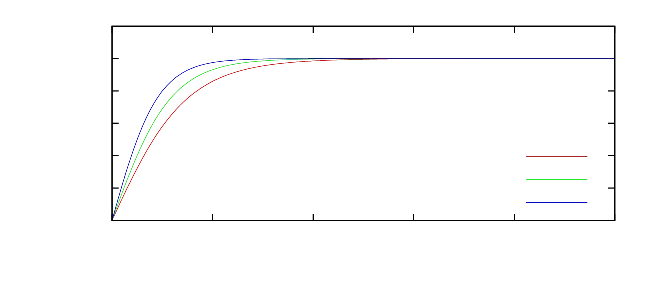
\includegraphics{vortex_func_f}}%
    \gplfronttext
  \end{picture}%
\endgroup

          \caption{\em Profile of the function $F(r)$ for a set of 3
            value for the $\lambda$ coupling constant. A numerical
            approximation of the function is obtained with a
            discretization of the interval $[0,10]$ into $N = 400$
            points. The BPS limit correspond to the green curve.}
          \label{fig:2d_vortex_f}
        \end{center}
      \end{figure}
      
      Fig. \ref{fig:2d_vortex_a} and \ref{fig:2d_vortex_f} show the
      profile of the two functions $A$ and $F$ for different values of
      the Higgs field coupling constant $\lambda$. The situation where
      $\lambda = 1$ correspond to the Bogomol'nyi-Prasad-Sommerfield
      limit (BPS limit).
    \end{subsubsection}
    \begin{subsubsection}{The Monopole in $(3+1)$ dimensions}\label{sec:theory_monopole}
      Let $\mathcal L$ be the Lagrangian of a $SU(2)$ gauge field
      theory, usually attributed to Georgi and Glashow:
      \begin{align}
        \mathcal L = -\frac{1}{4}F_{\mu\nu}^aF_{\mu\nu}^a+\frac{1}{2}(D_\mu\phi)^a(D_\mu\phi)^a-\frac{\lambda}{4}(\phi^a\phi^a-v^2)^2,
      \end{align}
      where $A_\mu$ and $\phi$ belongs to the $SU(2)$ algebra. t'Hooft
      and Polyakov have shown that there exists static solution with
      finite energy. Indeed, the most general static
      spherically symmetric solution can be written as:
      \begin{align}
        \phi^a(\vec r) = n^a v h(r),\\
        A_i^a(\vec r) = \frac{1}{gr}\varepsilon^{aij}n^jf(r),
      \end{align}
      where the finiteness of the energy imposes the following
      asymptotics for the two functions $f$ and $h$:
      \begin{align}
        f(0) = h(0) = 0,\\
        \lim_{r\to\infty} f(r) = \lim_{r\to\infty} h(r) = 1.
      \end{align}
      Substitution of this ansatz into the equations of motions leads
      to the following system of second order differential equations:
      \begin{align}
        r(rh''+2h')-2h(f-1)^2+\lambda v^2r^2h(1-h^2) = 0,\\
        r^2f'' = f(f-1)(f-2)+g^2 v^2 r^2 h^2(f-1).
      \end{align}
      It is convenient to perform the following change of field definitions:
      \begin{align}
        M(r):=rh(r)\Rightarrow M''(r)=rh''(r)+2h'(r),\\
        N(r):=1-f(r)\Rightarrow N''(r)=f''(r).
      \end{align}
      And the equations in terms of these new fields become:
      \begin{align}
        r^2M''(r)=2M(r)N(r)^2+\lambda v^2 M(r)(M(r)^2-r^2),\\
        r^2N''(r)=M(r)(M(r)^2-1)+gv^2N(r)^2M(r).
      \end{align}
      These equations are the ones that where originally derived by 't
      Hooft and Polyakov. This latter form was used in the numerical
      integration. As previously mentioned, a finite element method
      was used in order to find a numerical solution.

      The results of the integration of functions $M$ and $N$ is
      presented on Fig. \ref{fig:2d_monopole_f} and
      \ref{fig:2d_monopole_h}, for a set of three values of the Higgs
      coupling constant $\lambda$.
      \begin{figure}[!ht]
        \begin{center}
          % GNUPLOT: LaTeX picture with Postscript
\begingroup
  \makeatletter
  \providecommand\color[2][]{%
    \GenericError{(gnuplot) \space\space\space\@spaces}{%
      Package color not loaded in conjunction with
      terminal option `colourtext'%
    }{See the gnuplot documentation for explanation.%
    }{Either use 'blacktext' in gnuplot or load the package
      color.sty in LaTeX.}%
    \renewcommand\color[2][]{}%
  }%
  \providecommand\includegraphics[2][]{%
    \GenericError{(gnuplot) \space\space\space\@spaces}{%
      Package graphicx or graphics not loaded%
    }{See the gnuplot documentation for explanation.%
    }{The gnuplot epslatex terminal needs graphicx.sty or graphics.sty.}%
    \renewcommand\includegraphics[2][]{}%
  }%
  \providecommand\rotatebox[2]{#2}%
  \@ifundefined{ifGPcolor}{%
    \newif\ifGPcolor
    \GPcolortrue
  }{}%
  \@ifundefined{ifGPblacktext}{%
    \newif\ifGPblacktext
    \GPblacktexttrue
  }{}%
  % define a \g@addto@macro without @ in the name:
  \let\gplgaddtomacro\g@addto@macro
  % define empty templates for all commands taking text:
  \gdef\gplbacktext{}%
  \gdef\gplfronttext{}%
  \makeatother
  \ifGPblacktext
    % no textcolor at all
    \def\colorrgb#1{}%
    \def\colorgray#1{}%
  \else
    % gray or color?
    \ifGPcolor
      \def\colorrgb#1{\color[rgb]{#1}}%
      \def\colorgray#1{\color[gray]{#1}}%
      \expandafter\def\csname LTw\endcsname{\color{white}}%
      \expandafter\def\csname LTb\endcsname{\color{black}}%
      \expandafter\def\csname LTa\endcsname{\color{black}}%
      \expandafter\def\csname LT0\endcsname{\color[rgb]{1,0,0}}%
      \expandafter\def\csname LT1\endcsname{\color[rgb]{0,1,0}}%
      \expandafter\def\csname LT2\endcsname{\color[rgb]{0,0,1}}%
      \expandafter\def\csname LT3\endcsname{\color[rgb]{1,0,1}}%
      \expandafter\def\csname LT4\endcsname{\color[rgb]{0,1,1}}%
      \expandafter\def\csname LT5\endcsname{\color[rgb]{1,1,0}}%
      \expandafter\def\csname LT6\endcsname{\color[rgb]{0,0,0}}%
      \expandafter\def\csname LT7\endcsname{\color[rgb]{1,0.3,0}}%
      \expandafter\def\csname LT8\endcsname{\color[rgb]{0.5,0.5,0.5}}%
    \else
      % gray
      \def\colorrgb#1{\color{black}}%
      \def\colorgray#1{\color[gray]{#1}}%
      \expandafter\def\csname LTw\endcsname{\color{white}}%
      \expandafter\def\csname LTb\endcsname{\color{black}}%
      \expandafter\def\csname LTa\endcsname{\color{black}}%
      \expandafter\def\csname LT0\endcsname{\color{black}}%
      \expandafter\def\csname LT1\endcsname{\color{black}}%
      \expandafter\def\csname LT2\endcsname{\color{black}}%
      \expandafter\def\csname LT3\endcsname{\color{black}}%
      \expandafter\def\csname LT4\endcsname{\color{black}}%
      \expandafter\def\csname LT5\endcsname{\color{black}}%
      \expandafter\def\csname LT6\endcsname{\color{black}}%
      \expandafter\def\csname LT7\endcsname{\color{black}}%
      \expandafter\def\csname LT8\endcsname{\color{black}}%
    \fi
  \fi
  \setlength{\unitlength}{0.0500bp}%
  \begin{picture}(6236.00,2834.00)%
    \gplgaddtomacro\gplbacktext{%
      \csname LTb\endcsname%
      \put(1078,704){\makebox(0,0)[r]{\strut{} 0}}%
      \put(1078,1015){\makebox(0,0)[r]{\strut{} 0.2}}%
      \put(1078,1326){\makebox(0,0)[r]{\strut{} 0.4}}%
      \put(1078,1637){\makebox(0,0)[r]{\strut{} 0.6}}%
      \put(1078,1947){\makebox(0,0)[r]{\strut{} 0.8}}%
      \put(1078,2258){\makebox(0,0)[r]{\strut{} 1}}%
      \put(1210,484){\makebox(0,0){\strut{} 0}}%
      \put(1881,484){\makebox(0,0){\strut{} 1}}%
      \put(2551,484){\makebox(0,0){\strut{} 2}}%
      \put(3222,484){\makebox(0,0){\strut{} 3}}%
      \put(3893,484){\makebox(0,0){\strut{} 4}}%
      \put(4564,484){\makebox(0,0){\strut{} 5}}%
      \put(5234,484){\makebox(0,0){\strut{} 6}}%
      \put(5905,484){\makebox(0,0){\strut{} 7}}%
      \put(308,1636){\rotatebox{-270}{\makebox(0,0){\strut{}$N(r)\equiv 1-f(r)$}}}%
      \put(3557,154){\makebox(0,0){\strut{}$r$}}%
    }%
    \gplgaddtomacro\gplfronttext{%
      \csname LTb\endcsname%
      \put(4918,2396){\makebox(0,0)[r]{\strut{}$\lambda=0$}}%
      \csname LTb\endcsname%
      \put(4918,2176){\makebox(0,0)[r]{\strut{}$\lambda=0.5$}}%
      \csname LTb\endcsname%
      \put(4918,1956){\makebox(0,0)[r]{\strut{}$\lambda=1$}}%
    }%
    \gplbacktext
    \put(0,0){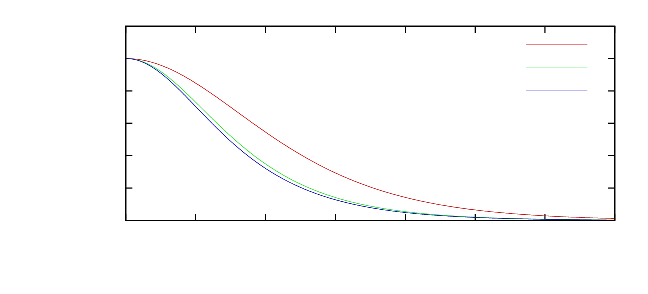
\includegraphics{monopole_funcs_a}}%
    \gplfronttext
  \end{picture}%
\endgroup

          \caption{\em Profile of the function $N(r)$ for a set of 3
            value for the $\lambda$ coupling constant. A numerical
            approximation of the function is obtained with a
            discretization of the interval $[0,10]$ into $N = 400$
            points. The BPS limit correspond to the red curve.}
          \label{fig:2d_monopole_f}
        \end{center}
      \end{figure}
      
      \begin{figure}[!ht]
        \begin{center}
          % GNUPLOT: LaTeX picture with Postscript
\begingroup
  \makeatletter
  \providecommand\color[2][]{%
    \GenericError{(gnuplot) \space\space\space\@spaces}{%
      Package color not loaded in conjunction with
      terminal option `colourtext'%
    }{See the gnuplot documentation for explanation.%
    }{Either use 'blacktext' in gnuplot or load the package
      color.sty in LaTeX.}%
    \renewcommand\color[2][]{}%
  }%
  \providecommand\includegraphics[2][]{%
    \GenericError{(gnuplot) \space\space\space\@spaces}{%
      Package graphicx or graphics not loaded%
    }{See the gnuplot documentation for explanation.%
    }{The gnuplot epslatex terminal needs graphicx.sty or graphics.sty.}%
    \renewcommand\includegraphics[2][]{}%
  }%
  \providecommand\rotatebox[2]{#2}%
  \@ifundefined{ifGPcolor}{%
    \newif\ifGPcolor
    \GPcolortrue
  }{}%
  \@ifundefined{ifGPblacktext}{%
    \newif\ifGPblacktext
    \GPblacktexttrue
  }{}%
  % define a \g@addto@macro without @ in the name:
  \let\gplgaddtomacro\g@addto@macro
  % define empty templates for all commands taking text:
  \gdef\gplbacktext{}%
  \gdef\gplfronttext{}%
  \makeatother
  \ifGPblacktext
    % no textcolor at all
    \def\colorrgb#1{}%
    \def\colorgray#1{}%
  \else
    % gray or color?
    \ifGPcolor
      \def\colorrgb#1{\color[rgb]{#1}}%
      \def\colorgray#1{\color[gray]{#1}}%
      \expandafter\def\csname LTw\endcsname{\color{white}}%
      \expandafter\def\csname LTb\endcsname{\color{black}}%
      \expandafter\def\csname LTa\endcsname{\color{black}}%
      \expandafter\def\csname LT0\endcsname{\color[rgb]{1,0,0}}%
      \expandafter\def\csname LT1\endcsname{\color[rgb]{0,1,0}}%
      \expandafter\def\csname LT2\endcsname{\color[rgb]{0,0,1}}%
      \expandafter\def\csname LT3\endcsname{\color[rgb]{1,0,1}}%
      \expandafter\def\csname LT4\endcsname{\color[rgb]{0,1,1}}%
      \expandafter\def\csname LT5\endcsname{\color[rgb]{1,1,0}}%
      \expandafter\def\csname LT6\endcsname{\color[rgb]{0,0,0}}%
      \expandafter\def\csname LT7\endcsname{\color[rgb]{1,0.3,0}}%
      \expandafter\def\csname LT8\endcsname{\color[rgb]{0.5,0.5,0.5}}%
    \else
      % gray
      \def\colorrgb#1{\color{black}}%
      \def\colorgray#1{\color[gray]{#1}}%
      \expandafter\def\csname LTw\endcsname{\color{white}}%
      \expandafter\def\csname LTb\endcsname{\color{black}}%
      \expandafter\def\csname LTa\endcsname{\color{black}}%
      \expandafter\def\csname LT0\endcsname{\color{black}}%
      \expandafter\def\csname LT1\endcsname{\color{black}}%
      \expandafter\def\csname LT2\endcsname{\color{black}}%
      \expandafter\def\csname LT3\endcsname{\color{black}}%
      \expandafter\def\csname LT4\endcsname{\color{black}}%
      \expandafter\def\csname LT5\endcsname{\color{black}}%
      \expandafter\def\csname LT6\endcsname{\color{black}}%
      \expandafter\def\csname LT7\endcsname{\color{black}}%
      \expandafter\def\csname LT8\endcsname{\color{black}}%
    \fi
  \fi
  \setlength{\unitlength}{0.0500bp}%
  \begin{picture}(6236.00,2834.00)%
    \gplgaddtomacro\gplbacktext{%
      \csname LTb\endcsname%
      \put(1078,704){\makebox(0,0)[r]{\strut{} 0}}%
      \put(1078,1015){\makebox(0,0)[r]{\strut{} 0.2}}%
      \put(1078,1326){\makebox(0,0)[r]{\strut{} 0.4}}%
      \put(1078,1637){\makebox(0,0)[r]{\strut{} 0.6}}%
      \put(1078,1947){\makebox(0,0)[r]{\strut{} 0.8}}%
      \put(1078,2258){\makebox(0,0)[r]{\strut{} 1}}%
      \put(1210,484){\makebox(0,0){\strut{} 0}}%
      \put(1881,484){\makebox(0,0){\strut{} 1}}%
      \put(2551,484){\makebox(0,0){\strut{} 2}}%
      \put(3222,484){\makebox(0,0){\strut{} 3}}%
      \put(3893,484){\makebox(0,0){\strut{} 4}}%
      \put(4564,484){\makebox(0,0){\strut{} 5}}%
      \put(5234,484){\makebox(0,0){\strut{} 6}}%
      \put(5905,484){\makebox(0,0){\strut{} 7}}%
      \put(308,1636){\rotatebox{-270}{\makebox(0,0){\strut{}$ f(r)$}}}%
      \put(3557,154){\makebox(0,0){\strut{}$r$}}%
    }%
    \gplgaddtomacro\gplfronttext{%
      \csname LTb\endcsname%
      \put(4918,1317){\makebox(0,0)[r]{\strut{}$\lambda=0$}}%
      \csname LTb\endcsname%
      \put(4918,1097){\makebox(0,0)[r]{\strut{}$\lambda=0.5$}}%
      \csname LTb\endcsname%
      \put(4918,877){\makebox(0,0)[r]{\strut{}$\lambda=1$}}%
    }%
    \gplbacktext
    \put(0,0){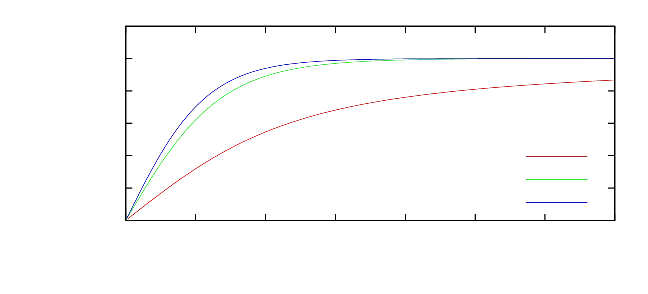
\includegraphics{monopole_funcs_f}}%
    \gplfronttext
  \end{picture}%
\endgroup

          \caption{\em Profile of the function $M(r)/r$ for a set of 3
            value for the $\lambda$ coupling constant.  We note that
            the asymptotic behaviour of the BPS limit case is note
            exponentially reaching 1 (red curve). In order to obtain a
            reasonable approximation, the boundary condition $M(r)/r =
            1$ must be imposed for a large radius. We used a
            discretization of the interval [0,100] into $N=3000$
            points.}
          \label{fig:2d_monopole_h}
        \end{center}
      \end{figure}
      The situation where $\lambda = 0$ correspond to the BPS limit,
      and is special in the sense that the solution can be expressed
      in terms of elementary functions:
      \begin{align}
        M(r) = \frac{r}{\tanh(r)}-1\quad ; \quad N(r) = \frac{r}{\sinh(r)}.
      \end{align}
      This situation is very valuable, since it gives a mean of
      checking the convergence of the analytic continuation in a
      very non trivial situation.
    \end{subsubsection}
  \end{subsection}
\end{section}
\begin{section}{Validity tests}
  Before using the procedure proposed in paragraph
  \ref{sec:numericalscheme}, we need to get convinced of its
  validity. For this purpose, we used a set of test case, where the
  solution is already known, and a closed form expression is
  available. One of the test cases is derived from a Sine-Gordon field
  equations.
  
  The method proposed attempt to compute the value of a function in
  some region of the complex plane, provided that we have a set of
  differential equations which describe the function, and its values
  known on a subset of the real axis.
  \begin{subsection}{Riemann sheet: the square root}
    We know try to find the analytic continuation of the square root
    on the complex plane:
    \begin{align}
      f(x) := \sqrt{x}.
    \end{align}
    The first step is to find a differential equation. This is easily achieved:
    \begin{align}
      &f'(x) = \frac{1}{2}x^{-1/2} = \frac{1}{2\sqrt{x}} = \frac{1}{2f(x)},\\
      \Rightarrow &f'(x) = \frac{1}{2f(x)}.\label{eq:squarediff}
    \end{align}
    If we know promote the function $f$ to be a complex number, using
    the Cauchy-Riemann equations (\ref{eq:cr}), we obtain the
    following system of differential equations:
    \begin{align}
      &\partial_xf_R(z)+i\partial_xf_I(z) = \frac{1}{2(f_R(z)+if_I(z))},\\
      &\Rightarrow 
      \left\{
      \begin{aligned}        
        &\partial_yf_I(z) = \frac{f_R(z)}{2(f_R^2(z)+f_I^2(z))},\\
        &-\partial_yf_R(z) = -\frac{f_I(z)}{2(f_R^2(z)+f_I^2(z))}.
      \end{aligned}
      \right.
    \end{align}
    with the initial conditions:
    \begin{align}
      &f_R(x+i0) = \sqrt{x},\\
      &f_I(x+i0) = 0.
    \end{align}
    We note that the function $-\sqrt{x}$ is also a solution of
    (\ref{eq:squarediff}). Obtaining the square root or its opposite
    is related to the choice of the initial conditions of the Cauchy
    problem.
    
    The result of the integration of the Cauchy problem is presented
    on Fig. \ref{fig:3d_sqrt}, for $\theta \in [0,4\pi]$. It is interesting to
    note that this procedure gives an access, at least in this case,
    to the complete Riemann manifold of the square root. The first
    $2\pi$ of the integration gives the upper sheet of the manifold,
    and the last $2\pi$ gives the lower sheet.
    
    \begin{figure}[!ht]
      \begin{center}
        % GNUPLOT: LaTeX picture with Postscript
\begingroup
\scriptsize
  \makeatletter
  \providecommand\color[2][]{%
    \GenericError{(gnuplot) \space\space\space\@spaces}{%
      Package color not loaded in conjunction with
      terminal option `colourtext'%
    }{See the gnuplot documentation for explanation.%
    }{Either use 'blacktext' in gnuplot or load the package
      color.sty in LaTeX.}%
    \renewcommand\color[2][]{}%
  }%
  \providecommand\includegraphics[2][]{%
    \GenericError{(gnuplot) \space\space\space\@spaces}{%
      Package graphicx or graphics not loaded%
    }{See the gnuplot documentation for explanation.%
    }{The gnuplot epslatex terminal needs graphicx.sty or graphics.sty.}%
    \renewcommand\includegraphics[2][]{}%
  }%
  \providecommand\rotatebox[2]{#2}%
  \@ifundefined{ifGPcolor}{%
    \newif\ifGPcolor
    \GPcolortrue
  }{}%
  \@ifundefined{ifGPblacktext}{%
    \newif\ifGPblacktext
    \GPblacktexttrue
  }{}%
  % define a \g@addto@macro without @ in the name:
  \let\gplgaddtomacro\g@addto@macro
  % define empty templates for all commands taking text:
  \gdef\gplbacktext{}%
  \gdef\gplfronttext{}%
  \makeatother
  \ifGPblacktext
    % no textcolor at all
    \def\colorrgb#1{}%
    \def\colorgray#1{}%
  \else
    % gray or color?
    \ifGPcolor
      \def\colorrgb#1{\color[rgb]{#1}}%
      \def\colorgray#1{\color[gray]{#1}}%
      \expandafter\def\csname LTw\endcsname{\color{white}}%
      \expandafter\def\csname LTb\endcsname{\color{black}}%
      \expandafter\def\csname LTa\endcsname{\color{black}}%
      \expandafter\def\csname LT0\endcsname{\color[rgb]{1,0,0}}%
      \expandafter\def\csname LT1\endcsname{\color[rgb]{0,1,0}}%
      \expandafter\def\csname LT2\endcsname{\color[rgb]{0,0,1}}%
      \expandafter\def\csname LT3\endcsname{\color[rgb]{1,0,1}}%
      \expandafter\def\csname LT4\endcsname{\color[rgb]{0,1,1}}%
      \expandafter\def\csname LT5\endcsname{\color[rgb]{1,1,0}}%
      \expandafter\def\csname LT6\endcsname{\color[rgb]{0,0,0}}%
      \expandafter\def\csname LT7\endcsname{\color[rgb]{1,0.3,0}}%
      \expandafter\def\csname LT8\endcsname{\color[rgb]{0.5,0.5,0.5}}%
    \else
      % gray
      \def\colorrgb#1{\color{black}}%
      \def\colorgray#1{\color[gray]{#1}}%
      \expandafter\def\csname LTw\endcsname{\color{white}}%
      \expandafter\def\csname LTb\endcsname{\color{black}}%
      \expandafter\def\csname LTa\endcsname{\color{black}}%
      \expandafter\def\csname LT0\endcsname{\color{black}}%
      \expandafter\def\csname LT1\endcsname{\color{black}}%
      \expandafter\def\csname LT2\endcsname{\color{black}}%
      \expandafter\def\csname LT3\endcsname{\color{black}}%
      \expandafter\def\csname LT4\endcsname{\color{black}}%
      \expandafter\def\csname LT5\endcsname{\color{black}}%
      \expandafter\def\csname LT6\endcsname{\color{black}}%
      \expandafter\def\csname LT7\endcsname{\color{black}}%
      \expandafter\def\csname LT8\endcsname{\color{black}}%
    \fi
  \fi
  \setlength{\unitlength}{0.0500bp}%
  \begin{picture}(2834.00,2834.00)%
    \gplgaddtomacro\gplbacktext{%
      \csname LTb\endcsname%
      \put(473,998){\makebox(0,0){\strut{}-1}}%
      \put(873,745){\makebox(0,0){\strut{} 0}}%
      \put(1273,491){\makebox(0,0){\strut{} 1}}%
      \put(1550,503){\makebox(0,0){\strut{}-1}}%
      \put(1950,756){\makebox(0,0){\strut{} 0}}%
      \put(2350,1009){\makebox(0,0){\strut{} 1}}%
      \put(411,1420){\makebox(0,0)[r]{\strut{}-1}}%
      \put(411,1658){\makebox(0,0)[r]{\strut{} 0}}%
      \put(411,1897){\makebox(0,0)[r]{\strut{} 1}}%
      \put(54,1358){\rotatebox{90}{\makebox(0,0){\strut{}$\Re\sqrt{x+iy}$}}}%
    }%
    \gplgaddtomacro\gplfronttext{%
      \csname LTb\endcsname%
      \put(626,496){\makebox(0,0){\strut{}$x$}}%
      \put(2209,496){\makebox(0,0){\strut{}$y$}}%
      \put(54,1358){\rotatebox{90}{\makebox(0,0){\strut{}$\Re\sqrt{x+iy}$}}}%
      \put(2517,1395){\makebox(0,0)[l]{\strut{}-1}}%
      \put(2517,1722){\makebox(0,0)[l]{\strut{} 0}}%
      \put(2517,2048){\makebox(0,0)[l]{\strut{} 1}}%
    }%
    \gplbacktext
    \put(0,0){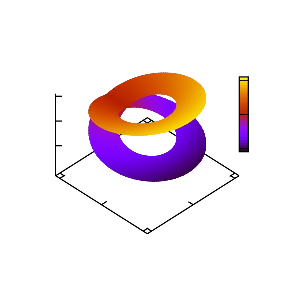
\includegraphics{sqrt_riemann_real}}%
    \gplfronttext
  \end{picture}%
\endgroup

        % GNUPLOT: LaTeX picture with Postscript
\begingroup
\scriptsize
  \makeatletter
  \providecommand\color[2][]{%
    \GenericError{(gnuplot) \space\space\space\@spaces}{%
      Package color not loaded in conjunction with
      terminal option `colourtext'%
    }{See the gnuplot documentation for explanation.%
    }{Either use 'blacktext' in gnuplot or load the package
      color.sty in LaTeX.}%
    \renewcommand\color[2][]{}%
  }%
  \providecommand\includegraphics[2][]{%
    \GenericError{(gnuplot) \space\space\space\@spaces}{%
      Package graphicx or graphics not loaded%
    }{See the gnuplot documentation for explanation.%
    }{The gnuplot epslatex terminal needs graphicx.sty or graphics.sty.}%
    \renewcommand\includegraphics[2][]{}%
  }%
  \providecommand\rotatebox[2]{#2}%
  \@ifundefined{ifGPcolor}{%
    \newif\ifGPcolor
    \GPcolortrue
  }{}%
  \@ifundefined{ifGPblacktext}{%
    \newif\ifGPblacktext
    \GPblacktexttrue
  }{}%
  % define a \g@addto@macro without @ in the name:
  \let\gplgaddtomacro\g@addto@macro
  % define empty templates for all commands taking text:
  \gdef\gplbacktext{}%
  \gdef\gplfronttext{}%
  \makeatother
  \ifGPblacktext
    % no textcolor at all
    \def\colorrgb#1{}%
    \def\colorgray#1{}%
  \else
    % gray or color?
    \ifGPcolor
      \def\colorrgb#1{\color[rgb]{#1}}%
      \def\colorgray#1{\color[gray]{#1}}%
      \expandafter\def\csname LTw\endcsname{\color{white}}%
      \expandafter\def\csname LTb\endcsname{\color{black}}%
      \expandafter\def\csname LTa\endcsname{\color{black}}%
      \expandafter\def\csname LT0\endcsname{\color[rgb]{1,0,0}}%
      \expandafter\def\csname LT1\endcsname{\color[rgb]{0,1,0}}%
      \expandafter\def\csname LT2\endcsname{\color[rgb]{0,0,1}}%
      \expandafter\def\csname LT3\endcsname{\color[rgb]{1,0,1}}%
      \expandafter\def\csname LT4\endcsname{\color[rgb]{0,1,1}}%
      \expandafter\def\csname LT5\endcsname{\color[rgb]{1,1,0}}%
      \expandafter\def\csname LT6\endcsname{\color[rgb]{0,0,0}}%
      \expandafter\def\csname LT7\endcsname{\color[rgb]{1,0.3,0}}%
      \expandafter\def\csname LT8\endcsname{\color[rgb]{0.5,0.5,0.5}}%
    \else
      % gray
      \def\colorrgb#1{\color{black}}%
      \def\colorgray#1{\color[gray]{#1}}%
      \expandafter\def\csname LTw\endcsname{\color{white}}%
      \expandafter\def\csname LTb\endcsname{\color{black}}%
      \expandafter\def\csname LTa\endcsname{\color{black}}%
      \expandafter\def\csname LT0\endcsname{\color{black}}%
      \expandafter\def\csname LT1\endcsname{\color{black}}%
      \expandafter\def\csname LT2\endcsname{\color{black}}%
      \expandafter\def\csname LT3\endcsname{\color{black}}%
      \expandafter\def\csname LT4\endcsname{\color{black}}%
      \expandafter\def\csname LT5\endcsname{\color{black}}%
      \expandafter\def\csname LT6\endcsname{\color{black}}%
      \expandafter\def\csname LT7\endcsname{\color{black}}%
      \expandafter\def\csname LT8\endcsname{\color{black}}%
    \fi
  \fi
  \setlength{\unitlength}{0.0500bp}%
  \begin{picture}(2834.00,2834.00)%
    \gplgaddtomacro\gplbacktext{%
      \csname LTb\endcsname%
      \put(473,998){\makebox(0,0){\strut{}-1}}%
      \put(873,745){\makebox(0,0){\strut{} 0}}%
      \put(1273,491){\makebox(0,0){\strut{} 1}}%
      \put(1550,503){\makebox(0,0){\strut{}-1}}%
      \put(1950,756){\makebox(0,0){\strut{} 0}}%
      \put(2350,1009){\makebox(0,0){\strut{} 1}}%
      \put(411,1420){\makebox(0,0)[r]{\strut{}-1}}%
      \put(411,1658){\makebox(0,0)[r]{\strut{} 0}}%
      \put(411,1897){\makebox(0,0)[r]{\strut{} 1}}%
      \put(54,1358){\rotatebox{90}{\makebox(0,0){\strut{}$\Im\sqrt{x+iy}$}}}%
    }%
    \gplgaddtomacro\gplfronttext{%
      \csname LTb\endcsname%
      \put(626,496){\makebox(0,0){\strut{}$x$}}%
      \put(2209,496){\makebox(0,0){\strut{}$y$}}%
      \put(54,1358){\rotatebox{90}{\makebox(0,0){\strut{}$\Im\sqrt{x+iy}$}}}%
      \put(2517,1395){\makebox(0,0)[l]{\strut{}-1}}%
      \put(2517,1722){\makebox(0,0)[l]{\strut{} 0}}%
      \put(2517,2048){\makebox(0,0)[l]{\strut{} 1}}%
    }%
    \gplbacktext
    \put(0,0){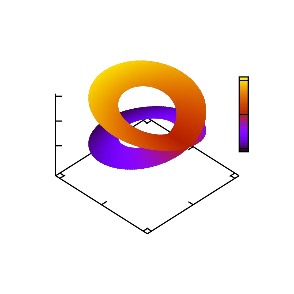
\includegraphics{sqrt_riemann_imag}}%
    \gplfronttext
  \end{picture}%
\endgroup

        \caption{\em Real (left) and imaginary (right) values of the
          analytic continuation of the square root function. The
          integration starts on the real axis, and ends exactly at the
          same place after two ($4\pi$) complete revolutions around
          the origin. The integration was performed using a polar
          coordinate system.}
        \label{fig:3d_sqrt}
      \end{center}
    \end{figure}
    The procedure is valid for this simple function, and converges to
    the continuation of the square root defined by:
    \begin{align}
      \sqrt{z} = \sqrt{\frac{\left|z\right|+\Re z}{2}}\pm i\sqrt{\frac{\left|z\right|-\Re z}{2}}.
    \end{align}
  \end{subsection}
  \begin{subsection}{The logarithm}
    It is now interesting to consider a function which presents a
    different type of singularity at the origin. The natural logarithm
    is a good candidate:
    \begin{align}
      f(x) := \log(x).
    \end{align}
    The corresponding differential equation is easily found as previously:
    \begin{align}
      f'(x) = \frac{1}{x} = \exp(-\log(x)) = \exp(-f(x)).
    \end{align}
    Promoting the $f$ function to be a complex number gives the
    following set of equations:
    \begin{align}
      \left\{
      \begin{aligned}
        &\partial_yf_I(z) = \exp(-f_R(z))\cos(f_I),\\
        &-\partial_yf_R(z) = -\exp(-f_R(z))\sin(f_I),
      \end{aligned}
      \right.
    \end{align}
    with the initial condition:
    \begin{align}
      \left\{
      \begin{aligned}
        &f_R(x+i0) = \log(x),\\
        &f_{I}(x+i0) = 0.
      \end{aligned}
      \right.
    \end{align}
    The result of the integration is presented on Fig. \ref{fig:3d_log}. As for
    the square root, we have access to the complete Riemann
    manifold. In these case, no particular branch cut is chosen or
    imposed by the procedure.
    \begin{figure}[!ht]
      \begin{center}
        % GNUPLOT: LaTeX picture with Postscript
\begingroup
\scriptsize
  \makeatletter
  \providecommand\color[2][]{%
    \GenericError{(gnuplot) \space\space\space\@spaces}{%
      Package color not loaded in conjunction with
      terminal option `colourtext'%
    }{See the gnuplot documentation for explanation.%
    }{Either use 'blacktext' in gnuplot or load the package
      color.sty in LaTeX.}%
    \renewcommand\color[2][]{}%
  }%
  \providecommand\includegraphics[2][]{%
    \GenericError{(gnuplot) \space\space\space\@spaces}{%
      Package graphicx or graphics not loaded%
    }{See the gnuplot documentation for explanation.%
    }{The gnuplot epslatex terminal needs graphicx.sty or graphics.sty.}%
    \renewcommand\includegraphics[2][]{}%
  }%
  \providecommand\rotatebox[2]{#2}%
  \@ifundefined{ifGPcolor}{%
    \newif\ifGPcolor
    \GPcolortrue
  }{}%
  \@ifundefined{ifGPblacktext}{%
    \newif\ifGPblacktext
    \GPblacktexttrue
  }{}%
  % define a \g@addto@macro without @ in the name:
  \let\gplgaddtomacro\g@addto@macro
  % define empty templates for all commands taking text:
  \gdef\gplbacktext{}%
  \gdef\gplfronttext{}%
  \makeatother
  \ifGPblacktext
    % no textcolor at all
    \def\colorrgb#1{}%
    \def\colorgray#1{}%
  \else
    % gray or color?
    \ifGPcolor
      \def\colorrgb#1{\color[rgb]{#1}}%
      \def\colorgray#1{\color[gray]{#1}}%
      \expandafter\def\csname LTw\endcsname{\color{white}}%
      \expandafter\def\csname LTb\endcsname{\color{black}}%
      \expandafter\def\csname LTa\endcsname{\color{black}}%
      \expandafter\def\csname LT0\endcsname{\color[rgb]{1,0,0}}%
      \expandafter\def\csname LT1\endcsname{\color[rgb]{0,1,0}}%
      \expandafter\def\csname LT2\endcsname{\color[rgb]{0,0,1}}%
      \expandafter\def\csname LT3\endcsname{\color[rgb]{1,0,1}}%
      \expandafter\def\csname LT4\endcsname{\color[rgb]{0,1,1}}%
      \expandafter\def\csname LT5\endcsname{\color[rgb]{1,1,0}}%
      \expandafter\def\csname LT6\endcsname{\color[rgb]{0,0,0}}%
      \expandafter\def\csname LT7\endcsname{\color[rgb]{1,0.3,0}}%
      \expandafter\def\csname LT8\endcsname{\color[rgb]{0.5,0.5,0.5}}%
    \else
      % gray
      \def\colorrgb#1{\color{black}}%
      \def\colorgray#1{\color[gray]{#1}}%
      \expandafter\def\csname LTw\endcsname{\color{white}}%
      \expandafter\def\csname LTb\endcsname{\color{black}}%
      \expandafter\def\csname LTa\endcsname{\color{black}}%
      \expandafter\def\csname LT0\endcsname{\color{black}}%
      \expandafter\def\csname LT1\endcsname{\color{black}}%
      \expandafter\def\csname LT2\endcsname{\color{black}}%
      \expandafter\def\csname LT3\endcsname{\color{black}}%
      \expandafter\def\csname LT4\endcsname{\color{black}}%
      \expandafter\def\csname LT5\endcsname{\color{black}}%
      \expandafter\def\csname LT6\endcsname{\color{black}}%
      \expandafter\def\csname LT7\endcsname{\color{black}}%
      \expandafter\def\csname LT8\endcsname{\color{black}}%
    \fi
  \fi
  \setlength{\unitlength}{0.0500bp}%
  \begin{picture}(2834.00,2834.00)%
    \gplgaddtomacro\gplbacktext{%
      \csname LTb\endcsname%
      \put(473,938){\makebox(0,0){\strut{}-1}}%
      \put(873,816){\makebox(0,0){\strut{} 0}}%
      \put(1273,693){\makebox(0,0){\strut{} 1}}%
      \put(1550,699){\makebox(0,0){\strut{}-1}}%
      \put(1950,821){\makebox(0,0){\strut{} 0}}%
      \put(2350,944){\makebox(0,0){\strut{} 1}}%
      \put(411,1385){\makebox(0,0)[r]{\strut{}-1}}%
      \put(411,1701){\makebox(0,0)[r]{\strut{} 0}}%
      \put(411,2019){\makebox(0,0)[r]{\strut{} 1}}%
      \put(54,1330){\rotatebox{90}{\makebox(0,0){\strut{}$\Re\log(x+iy)$}}}%
    }%
    \gplgaddtomacro\gplfronttext{%
      \csname LTb\endcsname%
      \put(626,582){\makebox(0,0){\strut{}$x$}}%
      \put(2209,582){\makebox(0,0){\strut{}$y$}}%
      \put(54,1330){\rotatebox{90}{\makebox(0,0){\strut{}$\Re\log(x+iy)$}}}%
      \put(2517,1363){\makebox(0,0)[l]{\strut{}-1}}%
      \put(2517,1722){\makebox(0,0)[l]{\strut{} 0}}%
      \put(2517,2081){\makebox(0,0)[l]{\strut{} 1}}%
    }%
    \gplbacktext
    \put(0,0){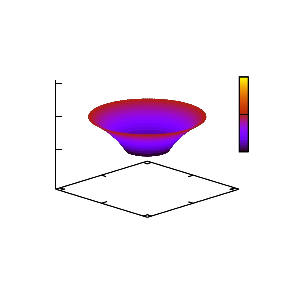
\includegraphics{log_riemann_real}}%
    \gplfronttext
  \end{picture}%
\endgroup

        % GNUPLOT: LaTeX picture with Postscript
\begingroup
\scriptsize
  \makeatletter
  \providecommand\color[2][]{%
    \GenericError{(gnuplot) \space\space\space\@spaces}{%
      Package color not loaded in conjunction with
      terminal option `colourtext'%
    }{See the gnuplot documentation for explanation.%
    }{Either use 'blacktext' in gnuplot or load the package
      color.sty in LaTeX.}%
    \renewcommand\color[2][]{}%
  }%
  \providecommand\includegraphics[2][]{%
    \GenericError{(gnuplot) \space\space\space\@spaces}{%
      Package graphicx or graphics not loaded%
    }{See the gnuplot documentation for explanation.%
    }{The gnuplot epslatex terminal needs graphicx.sty or graphics.sty.}%
    \renewcommand\includegraphics[2][]{}%
  }%
  \providecommand\rotatebox[2]{#2}%
  \@ifundefined{ifGPcolor}{%
    \newif\ifGPcolor
    \GPcolortrue
  }{}%
  \@ifundefined{ifGPblacktext}{%
    \newif\ifGPblacktext
    \GPblacktexttrue
  }{}%
  % define a \g@addto@macro without @ in the name:
  \let\gplgaddtomacro\g@addto@macro
  % define empty templates for all commands taking text:
  \gdef\gplbacktext{}%
  \gdef\gplfronttext{}%
  \makeatother
  \ifGPblacktext
    % no textcolor at all
    \def\colorrgb#1{}%
    \def\colorgray#1{}%
  \else
    % gray or color?
    \ifGPcolor
      \def\colorrgb#1{\color[rgb]{#1}}%
      \def\colorgray#1{\color[gray]{#1}}%
      \expandafter\def\csname LTw\endcsname{\color{white}}%
      \expandafter\def\csname LTb\endcsname{\color{black}}%
      \expandafter\def\csname LTa\endcsname{\color{black}}%
      \expandafter\def\csname LT0\endcsname{\color[rgb]{1,0,0}}%
      \expandafter\def\csname LT1\endcsname{\color[rgb]{0,1,0}}%
      \expandafter\def\csname LT2\endcsname{\color[rgb]{0,0,1}}%
      \expandafter\def\csname LT3\endcsname{\color[rgb]{1,0,1}}%
      \expandafter\def\csname LT4\endcsname{\color[rgb]{0,1,1}}%
      \expandafter\def\csname LT5\endcsname{\color[rgb]{1,1,0}}%
      \expandafter\def\csname LT6\endcsname{\color[rgb]{0,0,0}}%
      \expandafter\def\csname LT7\endcsname{\color[rgb]{1,0.3,0}}%
      \expandafter\def\csname LT8\endcsname{\color[rgb]{0.5,0.5,0.5}}%
    \else
      % gray
      \def\colorrgb#1{\color{black}}%
      \def\colorgray#1{\color[gray]{#1}}%
      \expandafter\def\csname LTw\endcsname{\color{white}}%
      \expandafter\def\csname LTb\endcsname{\color{black}}%
      \expandafter\def\csname LTa\endcsname{\color{black}}%
      \expandafter\def\csname LT0\endcsname{\color{black}}%
      \expandafter\def\csname LT1\endcsname{\color{black}}%
      \expandafter\def\csname LT2\endcsname{\color{black}}%
      \expandafter\def\csname LT3\endcsname{\color{black}}%
      \expandafter\def\csname LT4\endcsname{\color{black}}%
      \expandafter\def\csname LT5\endcsname{\color{black}}%
      \expandafter\def\csname LT6\endcsname{\color{black}}%
      \expandafter\def\csname LT7\endcsname{\color{black}}%
      \expandafter\def\csname LT8\endcsname{\color{black}}%
    \fi
  \fi
  \setlength{\unitlength}{0.0500bp}%
  \begin{picture}(2834.00,2834.00)%
    \gplgaddtomacro\gplbacktext{%
      \csname LTb\endcsname%
      \put(433,950){\makebox(0,0){\strut{}-1}}%
      \put(873,816){\makebox(0,0){\strut{} 0}}%
      \put(1313,681){\makebox(0,0){\strut{} 1}}%
      \put(1510,686){\makebox(0,0){\strut{}-1}}%
      \put(1950,821){\makebox(0,0){\strut{} 0}}%
      \put(2390,956){\makebox(0,0){\strut{} 1}}%
      \put(411,1357){\makebox(0,0)[r]{\strut{} 0}}%
      \put(411,1586){\makebox(0,0)[r]{\strut{} 5}}%
      \put(411,1816){\makebox(0,0)[r]{\strut{} 10}}%
      \put(411,2046){\makebox(0,0)[r]{\strut{} 15}}%
      \put(54,1330){\rotatebox{90}{\makebox(0,0){\strut{}$\Im\log(x+iy)$}}}%
    }%
    \gplgaddtomacro\gplfronttext{%
      \csname LTb\endcsname%
      \put(626,582){\makebox(0,0){\strut{}$x$}}%
      \put(2209,582){\makebox(0,0){\strut{}$y$}}%
      \put(54,1330){\rotatebox{90}{\makebox(0,0){\strut{}$\Im\log(x+iy)$}}}%
      \put(2517,1363){\makebox(0,0)[l]{\strut{} 0}}%
      \put(2517,1722){\makebox(0,0)[l]{\strut{} 7.5}}%
      \put(2517,2081){\makebox(0,0)[l]{\strut{} 15}}%
    }%
    \gplbacktext
    \put(0,0){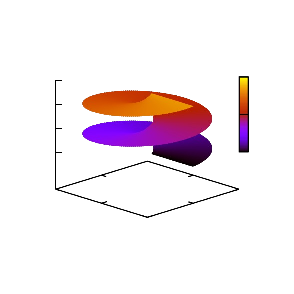
\includegraphics{log_riemann_imag}}%
    \gplfronttext
  \end{picture}%
\endgroup

        \caption{\em Real (left) and imaginary (right) values of the
          analytic continuation of the logarithm function. The
          integration was performed using a polar coordinate
          system. The integration starts on the real axis. The real
          component of $\log(z)$ for a given $|z|$. The imaginary part
          increase linearly with respect to $\theta$, increasing by
          $2\pi$ at each revolution around the origin.  }
        \label{fig:3d_log}
      \end{center}
    \end{figure}
    In this situation, in the range $\theta\in[-\pi,\pi]$ the
    numerical solution converges to
    \begin{align}
      \log(z) = \log(\left|z\right|)+i\arctan\left(\frac{y}{x}\right).
    \end{align}
  \end{subsection}
  \begin{subsection}{Quantum pendulum in gravitation}
    The last test case is less arbitrary, and in a sense related to the
    real problems to which we will eventually apply our analytic
    continuation procedure.
    
    Let's consider a pendulum in the field of gravity, which is
    described by the Lagrangian:
    \begin{align}
      \mathcal L = \frac{1}{2}\dot{\phi}^2-(\cos(\phi)-1).
    \end{align}
    We are interested in the instanton solution of the theory. The
    Hamiltonian is given by:
    \begin{align}
      h(t) = \frac{1}{2}\dot{\phi}^2+\cos(\phi).
    \end{align}
    It does not directly depends upon time, thus the energy is conserved. An
    instanton correspond to a trajectory which start at $\phi = 0$ and
    ends at $\phi = 2\pi$:
    \begin{align}
      \lim_{t\to-\infty} \phi(t) = 0\ ;\ \lim_{t\to \infty} \phi(t) = 2\pi.
    \end{align}
    In this situation, assuming that $\lim_{t\to-\infty}\dot{\phi} =
    0$ the Hamiltonian gives:
    \begin{align}
      h(t) = h = 0 = \frac{1}{2}\dot{\phi}^2+\cos(\phi)-1.
    \end{align}
    Integrating by separation of variables gives the solution for the
    time dependence of the instanton:
    \begin{align}
      \phi(t) = 4\arctan(\exp(t)).
    \end{align}
    The analytic continuation of this solution was computed using
    the second order equation of motion:
    \begin{align}
      \ddot\phi(t) = \sin(\phi(t)),
    \end{align}
    which must be recast into a first order equation, introducing a
    new variable:
    \begin{align}
      &\dot\phi(t) = \omega(t),\\
      &\dot\omega(t) = \sin(\phi(t)),
    \end{align}
    and the system to be integrated reads:
    \begin{align}
      \left\{
      \begin{aligned}
        \partial_y \phi_I &= \omega_R,\\
        \partial_y \omega_I &= \sin(\phi_R)\cosh(\phi_I),\\
        -\partial_y \phi_R &= \omega_I,\\
        -\partial_y \omega_R &= \cos(\phi_R)\sinh(\phi_I),
      \end{aligned}
      \right.
    \end{align}
    with initial conditions at $(t,y=0)$:
    \begin{align}
      \left\{
      \begin{aligned}
        &\phi_I(t+i0) = 0,\\
        &\omega_I(t+i0) = 0,\\
        &\phi_R(t+i0) = 4\arctan(\exp(t)),\\
        &\omega_R(t+i0) = \frac{4\exp(t)}{1+\exp(2t)}.
      \end{aligned}
      \right.
    \end{align}
    A qualitative view of the numerical results are provided by
    Fig. \ref{fig:3d_sine}, only for the first quadrant of the complex
    plane (which corresponds to the integration along the $\theta$
    polar coordinate from $0$ to $\pi/2$). We recognize on the $x$
    axis (real axis) of the real part of the analytic continuation,
    the profile of the instanton. Moreover, we clearly distinguish
    singularities regularly spaced on the imaginary axis. It is
    exactly what is expected by the analytic continuation of the
    function $4\arctan(\exp(z))$.

    \begin{figure}[!ht]
      \begin{center}
        % GNUPLOT: LaTeX picture with Postscript
\begingroup
\scriptsize
  \makeatletter
  \providecommand\color[2][]{%
    \GenericError{(gnuplot) \space\space\space\@spaces}{%
      Package color not loaded in conjunction with
      terminal option `colourtext'%
    }{See the gnuplot documentation for explanation.%
    }{Either use 'blacktext' in gnuplot or load the package
      color.sty in LaTeX.}%
    \renewcommand\color[2][]{}%
  }%
  \providecommand\includegraphics[2][]{%
    \GenericError{(gnuplot) \space\space\space\@spaces}{%
      Package graphicx or graphics not loaded%
    }{See the gnuplot documentation for explanation.%
    }{The gnuplot epslatex terminal needs graphicx.sty or graphics.sty.}%
    \renewcommand\includegraphics[2][]{}%
  }%
  \providecommand\rotatebox[2]{#2}%
  \@ifundefined{ifGPcolor}{%
    \newif\ifGPcolor
    \GPcolortrue
  }{}%
  \@ifundefined{ifGPblacktext}{%
    \newif\ifGPblacktext
    \GPblacktexttrue
  }{}%
  % define a \g@addto@macro without @ in the name:
  \let\gplgaddtomacro\g@addto@macro
  % define empty templates for all commands taking text:
  \gdef\gplbacktext{}%
  \gdef\gplfronttext{}%
  \makeatother
  \ifGPblacktext
    % no textcolor at all
    \def\colorrgb#1{}%
    \def\colorgray#1{}%
  \else
    % gray or color?
    \ifGPcolor
      \def\colorrgb#1{\color[rgb]{#1}}%
      \def\colorgray#1{\color[gray]{#1}}%
      \expandafter\def\csname LTw\endcsname{\color{white}}%
      \expandafter\def\csname LTb\endcsname{\color{black}}%
      \expandafter\def\csname LTa\endcsname{\color{black}}%
      \expandafter\def\csname LT0\endcsname{\color[rgb]{1,0,0}}%
      \expandafter\def\csname LT1\endcsname{\color[rgb]{0,1,0}}%
      \expandafter\def\csname LT2\endcsname{\color[rgb]{0,0,1}}%
      \expandafter\def\csname LT3\endcsname{\color[rgb]{1,0,1}}%
      \expandafter\def\csname LT4\endcsname{\color[rgb]{0,1,1}}%
      \expandafter\def\csname LT5\endcsname{\color[rgb]{1,1,0}}%
      \expandafter\def\csname LT6\endcsname{\color[rgb]{0,0,0}}%
      \expandafter\def\csname LT7\endcsname{\color[rgb]{1,0.3,0}}%
      \expandafter\def\csname LT8\endcsname{\color[rgb]{0.5,0.5,0.5}}%
    \else
      % gray
      \def\colorrgb#1{\color{black}}%
      \def\colorgray#1{\color[gray]{#1}}%
      \expandafter\def\csname LTw\endcsname{\color{white}}%
      \expandafter\def\csname LTb\endcsname{\color{black}}%
      \expandafter\def\csname LTa\endcsname{\color{black}}%
      \expandafter\def\csname LT0\endcsname{\color{black}}%
      \expandafter\def\csname LT1\endcsname{\color{black}}%
      \expandafter\def\csname LT2\endcsname{\color{black}}%
      \expandafter\def\csname LT3\endcsname{\color{black}}%
      \expandafter\def\csname LT4\endcsname{\color{black}}%
      \expandafter\def\csname LT5\endcsname{\color{black}}%
      \expandafter\def\csname LT6\endcsname{\color{black}}%
      \expandafter\def\csname LT7\endcsname{\color{black}}%
      \expandafter\def\csname LT8\endcsname{\color{black}}%
    \fi
  \fi
  \setlength{\unitlength}{0.0500bp}%
  \begin{picture}(2834.00,2834.00)%
    \gplgaddtomacro\gplbacktext{%
      \csname LTb\endcsname%
      \put(1521,573){\makebox(0,0){\strut{} 0}}%
      \put(1814,704){\makebox(0,0){\strut{} 3}}%
      \put(2108,836){\makebox(0,0){\strut{} 6}}%
      \put(2401,967){\makebox(0,0){\strut{} 9}}%
      \put(1324,581){\makebox(0,0){\strut{} 0}}%
      \put(1031,712){\makebox(0,0){\strut{} 3}}%
      \put(737,844){\makebox(0,0){\strut{} 6}}%
      \put(444,975){\makebox(0,0){\strut{} 9}}%
      \put(411,1447){\makebox(0,0)[r]{\strut{} 3}}%
      \put(411,1687){\makebox(0,0)[r]{\strut{} 6}}%
      \put(411,1929){\makebox(0,0)[r]{\strut{} 9}}%
      \put(54,1589){\rotatebox{90}{\makebox(0,0){\strut{}$\Re\ 4\mathrm{atan}(e^{x+iy})$}}}%
    }%
    \gplgaddtomacro\gplfronttext{%
      \csname LTb\endcsname%
      \put(2209,530){\makebox(0,0){\strut{}$x$}}%
      \put(626,530){\makebox(0,0){\strut{}$y$}}%
      \put(54,1589){\rotatebox{90}{\makebox(0,0){\strut{}$\Re\ 4\mathrm{atan}(e^{x+iy})$}}}%
      \put(2517,1452){\makebox(0,0)[l]{\strut{} 3}}%
      \put(2517,1722){\makebox(0,0)[l]{\strut{} 6}}%
      \put(2517,1991){\makebox(0,0)[l]{\strut{} 9}}%
    }%
    \gplbacktext
    \put(0,0){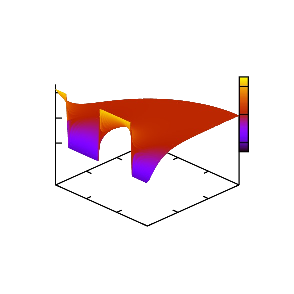
\includegraphics{sine_quadrant_real}}%
    \gplfronttext
  \end{picture}%
\endgroup

        % GNUPLOT: LaTeX picture with Postscript
\begingroup
\scriptsize
  \makeatletter
  \providecommand\color[2][]{%
    \GenericError{(gnuplot) \space\space\space\@spaces}{%
      Package color not loaded in conjunction with
      terminal option `colourtext'%
    }{See the gnuplot documentation for explanation.%
    }{Either use 'blacktext' in gnuplot or load the package
      color.sty in LaTeX.}%
    \renewcommand\color[2][]{}%
  }%
  \providecommand\includegraphics[2][]{%
    \GenericError{(gnuplot) \space\space\space\@spaces}{%
      Package graphicx or graphics not loaded%
    }{See the gnuplot documentation for explanation.%
    }{The gnuplot epslatex terminal needs graphicx.sty or graphics.sty.}%
    \renewcommand\includegraphics[2][]{}%
  }%
  \providecommand\rotatebox[2]{#2}%
  \@ifundefined{ifGPcolor}{%
    \newif\ifGPcolor
    \GPcolortrue
  }{}%
  \@ifundefined{ifGPblacktext}{%
    \newif\ifGPblacktext
    \GPblacktexttrue
  }{}%
  % define a \g@addto@macro without @ in the name:
  \let\gplgaddtomacro\g@addto@macro
  % define empty templates for all commands taking text:
  \gdef\gplbacktext{}%
  \gdef\gplfronttext{}%
  \makeatother
  \ifGPblacktext
    % no textcolor at all
    \def\colorrgb#1{}%
    \def\colorgray#1{}%
  \else
    % gray or color?
    \ifGPcolor
      \def\colorrgb#1{\color[rgb]{#1}}%
      \def\colorgray#1{\color[gray]{#1}}%
      \expandafter\def\csname LTw\endcsname{\color{white}}%
      \expandafter\def\csname LTb\endcsname{\color{black}}%
      \expandafter\def\csname LTa\endcsname{\color{black}}%
      \expandafter\def\csname LT0\endcsname{\color[rgb]{1,0,0}}%
      \expandafter\def\csname LT1\endcsname{\color[rgb]{0,1,0}}%
      \expandafter\def\csname LT2\endcsname{\color[rgb]{0,0,1}}%
      \expandafter\def\csname LT3\endcsname{\color[rgb]{1,0,1}}%
      \expandafter\def\csname LT4\endcsname{\color[rgb]{0,1,1}}%
      \expandafter\def\csname LT5\endcsname{\color[rgb]{1,1,0}}%
      \expandafter\def\csname LT6\endcsname{\color[rgb]{0,0,0}}%
      \expandafter\def\csname LT7\endcsname{\color[rgb]{1,0.3,0}}%
      \expandafter\def\csname LT8\endcsname{\color[rgb]{0.5,0.5,0.5}}%
    \else
      % gray
      \def\colorrgb#1{\color{black}}%
      \def\colorgray#1{\color[gray]{#1}}%
      \expandafter\def\csname LTw\endcsname{\color{white}}%
      \expandafter\def\csname LTb\endcsname{\color{black}}%
      \expandafter\def\csname LTa\endcsname{\color{black}}%
      \expandafter\def\csname LT0\endcsname{\color{black}}%
      \expandafter\def\csname LT1\endcsname{\color{black}}%
      \expandafter\def\csname LT2\endcsname{\color{black}}%
      \expandafter\def\csname LT3\endcsname{\color{black}}%
      \expandafter\def\csname LT4\endcsname{\color{black}}%
      \expandafter\def\csname LT5\endcsname{\color{black}}%
      \expandafter\def\csname LT6\endcsname{\color{black}}%
      \expandafter\def\csname LT7\endcsname{\color{black}}%
      \expandafter\def\csname LT8\endcsname{\color{black}}%
    \fi
  \fi
  \setlength{\unitlength}{0.0500bp}%
  \begin{picture}(2834.00,2834.00)%
    \gplgaddtomacro\gplbacktext{%
      \csname LTb\endcsname%
      \put(1521,573){\makebox(0,0){\strut{} 0}}%
      \put(1814,704){\makebox(0,0){\strut{} 3}}%
      \put(2108,836){\makebox(0,0){\strut{} 6}}%
      \put(2401,967){\makebox(0,0){\strut{} 9}}%
      \put(1324,581){\makebox(0,0){\strut{} 0}}%
      \put(1031,712){\makebox(0,0){\strut{} 3}}%
      \put(737,844){\makebox(0,0){\strut{} 6}}%
      \put(444,975){\makebox(0,0){\strut{} 9}}%
      \put(411,1367){\makebox(0,0)[r]{\strut{}-8}}%
      \put(411,1687){\makebox(0,0)[r]{\strut{} 0}}%
      \put(411,2009){\makebox(0,0)[r]{\strut{} 8}}%
      \put(54,1589){\rotatebox{90}{\makebox(0,0){\strut{}$\Im\ 4\mathrm{atan}(e^{x+iy})$}}}%
    }%
    \gplgaddtomacro\gplfronttext{%
      \csname LTb\endcsname%
      \put(2209,530){\makebox(0,0){\strut{}$x$}}%
      \put(626,530){\makebox(0,0){\strut{}$y$}}%
      \put(54,1589){\rotatebox{90}{\makebox(0,0){\strut{}$\Im\ 4\mathrm{atan}(e^{x+iy})$}}}%
      \put(2517,1363){\makebox(0,0)[l]{\strut{}-8}}%
      \put(2517,1722){\makebox(0,0)[l]{\strut{} 0}}%
      \put(2517,2081){\makebox(0,0)[l]{\strut{} 8}}%
    }%
    \gplbacktext
    \put(0,0){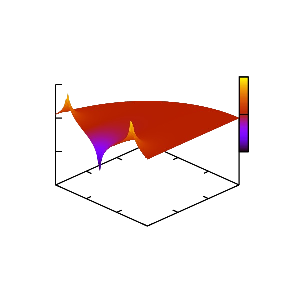
\includegraphics{sine_quadrant_imag}}%
    \gplfronttext
  \end{picture}%
\endgroup

        \caption{\em Real (left) and imaginary (right) parts of the
          analytic continuation of the solution. We distinguish the
          first 3 singularities on the positive imaginary axis, at
          $i\pi/2$, $i3\pi/2$, $i5\pi/2$. A polar coordinate system was
          used for the integration.}
        \label{fig:3d_sine} 
      \end{center}
    \end{figure}

    Fig. \ref{fig:cm_sine_real} and \ref{fig:cm_sine_imag} show the real and imaginary parts of the solution. We clearly distinguish the singularities on the
    imaginary axis. There are infinitely many of them, located at
    $(2n+1)\pi/2, n=0,1,\dots$. We also notice the formation of a
    discontinuity after each one of them on the real part of the
    function.

    This example demonstrates one interesting feature of the
    procedure of analytic continuation. It can be shown that the
    singularities on the imaginary axis are of the same type as the
    singularity at the origin for the logarithm. The choice of a
    coordinate system imposes naturally a set of coordinate paths, and
    the result of the integration along these paths depends on the
    singularities which lie on each side of the paths.
    
    For this reason, the branch cuts appear naturally along the
    coordinate lines.
    \begin{figure}[!ht]
      \begin{center}
        % GNUPLOT: LaTeX picture with Postscript
\begingroup
  \makeatletter
  \providecommand\color[2][]{%
    \GenericError{(gnuplot) \space\space\space\@spaces}{%
      Package color not loaded in conjunction with
      terminal option `colourtext'%
    }{See the gnuplot documentation for explanation.%
    }{Either use 'blacktext' in gnuplot or load the package
      color.sty in LaTeX.}%
    \renewcommand\color[2][]{}%
  }%
  \providecommand\includegraphics[2][]{%
    \GenericError{(gnuplot) \space\space\space\@spaces}{%
      Package graphicx or graphics not loaded%
    }{See the gnuplot documentation for explanation.%
    }{The gnuplot epslatex terminal needs graphicx.sty or graphics.sty.}%
    \renewcommand\includegraphics[2][]{}%
  }%
  \providecommand\rotatebox[2]{#2}%
  \@ifundefined{ifGPcolor}{%
    \newif\ifGPcolor
    \GPcolortrue
  }{}%
  \@ifundefined{ifGPblacktext}{%
    \newif\ifGPblacktext
    \GPblacktexttrue
  }{}%
  % define a \g@addto@macro without @ in the name:
  \let\gplgaddtomacro\g@addto@macro
  % define empty templates for all commands taking text:
  \gdef\gplbacktext{}%
  \gdef\gplfronttext{}%
  \makeatother
  \ifGPblacktext
    % no textcolor at all
    \def\colorrgb#1{}%
    \def\colorgray#1{}%
  \else
    % gray or color?
    \ifGPcolor
      \def\colorrgb#1{\color[rgb]{#1}}%
      \def\colorgray#1{\color[gray]{#1}}%
      \expandafter\def\csname LTw\endcsname{\color{white}}%
      \expandafter\def\csname LTb\endcsname{\color{black}}%
      \expandafter\def\csname LTa\endcsname{\color{black}}%
      \expandafter\def\csname LT0\endcsname{\color[rgb]{1,0,0}}%
      \expandafter\def\csname LT1\endcsname{\color[rgb]{0,1,0}}%
      \expandafter\def\csname LT2\endcsname{\color[rgb]{0,0,1}}%
      \expandafter\def\csname LT3\endcsname{\color[rgb]{1,0,1}}%
      \expandafter\def\csname LT4\endcsname{\color[rgb]{0,1,1}}%
      \expandafter\def\csname LT5\endcsname{\color[rgb]{1,1,0}}%
      \expandafter\def\csname LT6\endcsname{\color[rgb]{0,0,0}}%
      \expandafter\def\csname LT7\endcsname{\color[rgb]{1,0.3,0}}%
      \expandafter\def\csname LT8\endcsname{\color[rgb]{0.5,0.5,0.5}}%
    \else
      % gray
      \def\colorrgb#1{\color{black}}%
      \def\colorgray#1{\color[gray]{#1}}%
      \expandafter\def\csname LTw\endcsname{\color{white}}%
      \expandafter\def\csname LTb\endcsname{\color{black}}%
      \expandafter\def\csname LTa\endcsname{\color{black}}%
      \expandafter\def\csname LT0\endcsname{\color{black}}%
      \expandafter\def\csname LT1\endcsname{\color{black}}%
      \expandafter\def\csname LT2\endcsname{\color{black}}%
      \expandafter\def\csname LT3\endcsname{\color{black}}%
      \expandafter\def\csname LT4\endcsname{\color{black}}%
      \expandafter\def\csname LT5\endcsname{\color{black}}%
      \expandafter\def\csname LT6\endcsname{\color{black}}%
      \expandafter\def\csname LT7\endcsname{\color{black}}%
      \expandafter\def\csname LT8\endcsname{\color{black}}%
    \fi
  \fi
  \setlength{\unitlength}{0.0500bp}%
  \begin{picture}(6236.00,2834.00)%
    \gplgaddtomacro\gplbacktext{%
    }%
    \gplgaddtomacro\gplfronttext{%
      \csname LTb\endcsname%
      \put(1139,517){\makebox(0,0){\strut{}-9}}%
      \put(1799,517){\makebox(0,0){\strut{}-6}}%
      \put(2459,517){\makebox(0,0){\strut{}-3}}%
      \put(3118,517){\makebox(0,0){\strut{} 0}}%
      \put(3777,517){\makebox(0,0){\strut{} 3}}%
      \put(4437,517){\makebox(0,0){\strut{} 6}}%
      \put(5097,517){\makebox(0,0){\strut{} 9}}%
      \put(3118,187){\makebox(0,0){\strut{}$x$}}%
      \put(874,803){\makebox(0,0)[r]{\strut{} 0}}%
      \put(874,1264){\makebox(0,0)[r]{\strut{} 3}}%
      \put(874,1725){\makebox(0,0)[r]{\strut{} 6}}%
      \put(874,2186){\makebox(0,0)[r]{\strut{} 9}}%
      \put(544,1527){\rotatebox{-270}{\makebox(0,0){\strut{}$y$}}}%
      \put(5633,802){\makebox(0,0)[l]{\strut{} 0}}%
      \put(5633,1526){\makebox(0,0)[l]{\strut{} 6.28319}}%
      \put(5633,2251){\makebox(0,0)[l]{\strut{} 12.5664}}%
    }%
    \gplbacktext
    \put(0,0){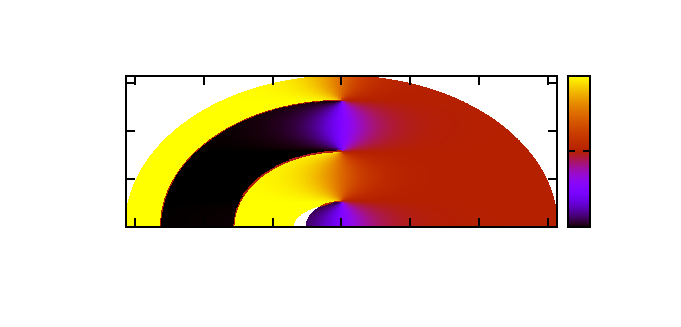
\includegraphics{sine_real}}%
    \gplfronttext
  \end{picture}%
\endgroup

        \caption{\em Real part of the solution in the positive
          imaginary half plane. The solution is the same in the
          negative half plane. We clearly see the branch cut starting
          from each singularity.}
        \label{fig:cm_sine_real}
      \end{center}
    \end{figure}

    \begin{figure}[!ht]
      \begin{center}
        % GNUPLOT: LaTeX picture with Postscript
\begingroup
  \makeatletter
  \providecommand\color[2][]{%
    \GenericError{(gnuplot) \space\space\space\@spaces}{%
      Package color not loaded in conjunction with
      terminal option `colourtext'%
    }{See the gnuplot documentation for explanation.%
    }{Either use 'blacktext' in gnuplot or load the package
      color.sty in LaTeX.}%
    \renewcommand\color[2][]{}%
  }%
  \providecommand\includegraphics[2][]{%
    \GenericError{(gnuplot) \space\space\space\@spaces}{%
      Package graphicx or graphics not loaded%
    }{See the gnuplot documentation for explanation.%
    }{The gnuplot epslatex terminal needs graphicx.sty or graphics.sty.}%
    \renewcommand\includegraphics[2][]{}%
  }%
  \providecommand\rotatebox[2]{#2}%
  \@ifundefined{ifGPcolor}{%
    \newif\ifGPcolor
    \GPcolortrue
  }{}%
  \@ifundefined{ifGPblacktext}{%
    \newif\ifGPblacktext
    \GPblacktexttrue
  }{}%
  % define a \g@addto@macro without @ in the name:
  \let\gplgaddtomacro\g@addto@macro
  % define empty templates for all commands taking text:
  \gdef\gplbacktext{}%
  \gdef\gplfronttext{}%
  \makeatother
  \ifGPblacktext
    % no textcolor at all
    \def\colorrgb#1{}%
    \def\colorgray#1{}%
  \else
    % gray or color?
    \ifGPcolor
      \def\colorrgb#1{\color[rgb]{#1}}%
      \def\colorgray#1{\color[gray]{#1}}%
      \expandafter\def\csname LTw\endcsname{\color{white}}%
      \expandafter\def\csname LTb\endcsname{\color{black}}%
      \expandafter\def\csname LTa\endcsname{\color{black}}%
      \expandafter\def\csname LT0\endcsname{\color[rgb]{1,0,0}}%
      \expandafter\def\csname LT1\endcsname{\color[rgb]{0,1,0}}%
      \expandafter\def\csname LT2\endcsname{\color[rgb]{0,0,1}}%
      \expandafter\def\csname LT3\endcsname{\color[rgb]{1,0,1}}%
      \expandafter\def\csname LT4\endcsname{\color[rgb]{0,1,1}}%
      \expandafter\def\csname LT5\endcsname{\color[rgb]{1,1,0}}%
      \expandafter\def\csname LT6\endcsname{\color[rgb]{0,0,0}}%
      \expandafter\def\csname LT7\endcsname{\color[rgb]{1,0.3,0}}%
      \expandafter\def\csname LT8\endcsname{\color[rgb]{0.5,0.5,0.5}}%
    \else
      % gray
      \def\colorrgb#1{\color{black}}%
      \def\colorgray#1{\color[gray]{#1}}%
      \expandafter\def\csname LTw\endcsname{\color{white}}%
      \expandafter\def\csname LTb\endcsname{\color{black}}%
      \expandafter\def\csname LTa\endcsname{\color{black}}%
      \expandafter\def\csname LT0\endcsname{\color{black}}%
      \expandafter\def\csname LT1\endcsname{\color{black}}%
      \expandafter\def\csname LT2\endcsname{\color{black}}%
      \expandafter\def\csname LT3\endcsname{\color{black}}%
      \expandafter\def\csname LT4\endcsname{\color{black}}%
      \expandafter\def\csname LT5\endcsname{\color{black}}%
      \expandafter\def\csname LT6\endcsname{\color{black}}%
      \expandafter\def\csname LT7\endcsname{\color{black}}%
      \expandafter\def\csname LT8\endcsname{\color{black}}%
    \fi
  \fi
  \setlength{\unitlength}{0.0500bp}%
  \begin{picture}(6236.00,2834.00)%
    \gplgaddtomacro\gplbacktext{%
    }%
    \gplgaddtomacro\gplfronttext{%
      \csname LTb\endcsname%
      \put(1139,517){\makebox(0,0){\strut{}-9}}%
      \put(1799,517){\makebox(0,0){\strut{}-6}}%
      \put(2459,517){\makebox(0,0){\strut{}-3}}%
      \put(3118,517){\makebox(0,0){\strut{} 0}}%
      \put(3777,517){\makebox(0,0){\strut{} 3}}%
      \put(4437,517){\makebox(0,0){\strut{} 6}}%
      \put(5097,517){\makebox(0,0){\strut{} 9}}%
      \put(3118,187){\makebox(0,0){\strut{}$x$}}%
      \put(874,803){\makebox(0,0)[r]{\strut{} 0}}%
      \put(874,1264){\makebox(0,0)[r]{\strut{} 3}}%
      \put(874,1725){\makebox(0,0)[r]{\strut{} 6}}%
      \put(874,2186){\makebox(0,0)[r]{\strut{} 9}}%
      \put(544,1527){\rotatebox{-270}{\makebox(0,0){\strut{}$y$}}}%
      \put(5633,802){\makebox(0,0)[l]{\strut{}-5}}%
      \put(5633,1526){\makebox(0,0)[l]{\strut{} 0}}%
      \put(5633,2251){\makebox(0,0)[l]{\strut{} 5}}%
    }%
    \gplbacktext
    \put(0,0){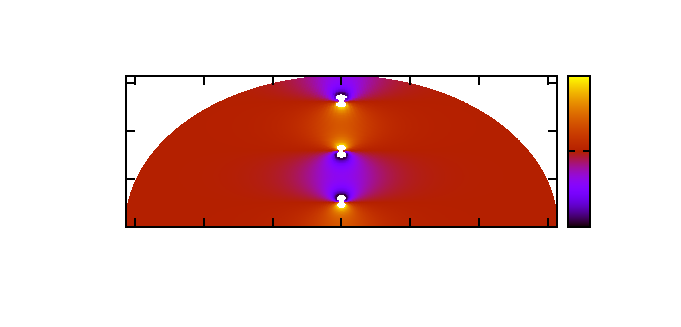
\includegraphics{sine_imag}}%
    \gplfronttext
  \end{picture}%
\endgroup

        \caption{\em Imaginary part of the solution in the positive
          imaginary half plane.}
        \label{fig:cm_sine_imag}
      \end{center}
    \end{figure}

    Finally, Fig. \ref{fig:2d_sine_diff} shows the behaviour of the
    function in the vicinity of a singularity. The difference of the
    value of the function along two paths is represented. The first
    path passes at a distance $\Delta$ below the first singularity
    on the positive imaginary axis, and the second path passes at a
    distance $\Delta$ above the same singularity. Ideally $\Delta\to
    0$ but it is numerically not feasible.
    \begin{figure}[!ht]
      \begin{center}
        % GNUPLOT: LaTeX picture with Postscript
\begingroup
\scriptsize
  \makeatletter
  \providecommand\color[2][]{%
    \GenericError{(gnuplot) \space\space\space\@spaces}{%
      Package color not loaded in conjunction with
      terminal option `colourtext'%
    }{See the gnuplot documentation for explanation.%
    }{Either use 'blacktext' in gnuplot or load the package
      color.sty in LaTeX.}%
    \renewcommand\color[2][]{}%
  }%
  \providecommand\includegraphics[2][]{%
    \GenericError{(gnuplot) \space\space\space\@spaces}{%
      Package graphicx or graphics not loaded%
    }{See the gnuplot documentation for explanation.%
    }{The gnuplot epslatex terminal needs graphicx.sty or graphics.sty.}%
    \renewcommand\includegraphics[2][]{}%
  }%
  \providecommand\rotatebox[2]{#2}%
  \@ifundefined{ifGPcolor}{%
    \newif\ifGPcolor
    \GPcolortrue
  }{}%
  \@ifundefined{ifGPblacktext}{%
    \newif\ifGPblacktext
    \GPblacktexttrue
  }{}%
  % define a \g@addto@macro without @ in the name:
  \let\gplgaddtomacro\g@addto@macro
  % define empty templates for all commands taking text:
  \gdef\gplbacktext{}%
  \gdef\gplfronttext{}%
  \makeatother
  \ifGPblacktext
    % no textcolor at all
    \def\colorrgb#1{}%
    \def\colorgray#1{}%
  \else
    % gray or color?
    \ifGPcolor
      \def\colorrgb#1{\color[rgb]{#1}}%
      \def\colorgray#1{\color[gray]{#1}}%
      \expandafter\def\csname LTw\endcsname{\color{white}}%
      \expandafter\def\csname LTb\endcsname{\color{black}}%
      \expandafter\def\csname LTa\endcsname{\color{black}}%
      \expandafter\def\csname LT0\endcsname{\color[rgb]{1,0,0}}%
      \expandafter\def\csname LT1\endcsname{\color[rgb]{0,1,0}}%
      \expandafter\def\csname LT2\endcsname{\color[rgb]{0,0,1}}%
      \expandafter\def\csname LT3\endcsname{\color[rgb]{1,0,1}}%
      \expandafter\def\csname LT4\endcsname{\color[rgb]{0,1,1}}%
      \expandafter\def\csname LT5\endcsname{\color[rgb]{1,1,0}}%
      \expandafter\def\csname LT6\endcsname{\color[rgb]{0,0,0}}%
      \expandafter\def\csname LT7\endcsname{\color[rgb]{1,0.3,0}}%
      \expandafter\def\csname LT8\endcsname{\color[rgb]{0.5,0.5,0.5}}%
    \else
      % gray
      \def\colorrgb#1{\color{black}}%
      \def\colorgray#1{\color[gray]{#1}}%
      \expandafter\def\csname LTw\endcsname{\color{white}}%
      \expandafter\def\csname LTb\endcsname{\color{black}}%
      \expandafter\def\csname LTa\endcsname{\color{black}}%
      \expandafter\def\csname LT0\endcsname{\color{black}}%
      \expandafter\def\csname LT1\endcsname{\color{black}}%
      \expandafter\def\csname LT2\endcsname{\color{black}}%
      \expandafter\def\csname LT3\endcsname{\color{black}}%
      \expandafter\def\csname LT4\endcsname{\color{black}}%
      \expandafter\def\csname LT5\endcsname{\color{black}}%
      \expandafter\def\csname LT6\endcsname{\color{black}}%
      \expandafter\def\csname LT7\endcsname{\color{black}}%
      \expandafter\def\csname LT8\endcsname{\color{black}}%
    \fi
  \fi
  \setlength{\unitlength}{0.0500bp}%
  \begin{picture}(6236.00,2834.00)%
    \gplgaddtomacro\gplbacktext{%
      \csname LTb\endcsname%
      \put(1386,911){\makebox(0,0)[r]{\strut{} 0}}%
      \put(1386,1562){\makebox(0,0)[r]{\strut{} 6.28319}}%
      \put(1386,2213){\makebox(0,0)[r]{\strut{} 12.5664}}%
      \put(1518,484){\makebox(0,0){\strut{} 0.5}}%
      \put(2542,484){\makebox(0,0){\strut{} 1}}%
      \put(3566,484){\makebox(0,0){\strut{} 1.5}}%
      \put(4591,484){\makebox(0,0){\strut{} 2}}%
      \put(5615,484){\makebox(0,0){\strut{} 2.5}}%
      \put(352,1636){\rotatebox{-270}{\makebox(0,0){\strut{}$\phi_R(\pi/2+\Delta,\theta)-\phi_R(\pi/2-\Delta,\theta)$}}}%
      \put(3711,154){\makebox(0,0){\strut{}$\theta$}}%
    }%
    \gplgaddtomacro\gplfronttext{%
      \csname LTb\endcsname%
      \put(4918,1317){\makebox(0,0)[r]{\strut{}$\Delta=0.01$}}%
      \csname LTb\endcsname%
      \put(4918,1097){\makebox(0,0)[r]{\strut{}$\Delta=0.005$}}%
      \csname LTb\endcsname%
      \put(4918,877){\makebox(0,0)[r]{\strut{}$\Delta=0.001$}}%
    }%
    \gplbacktext
    \put(0,0){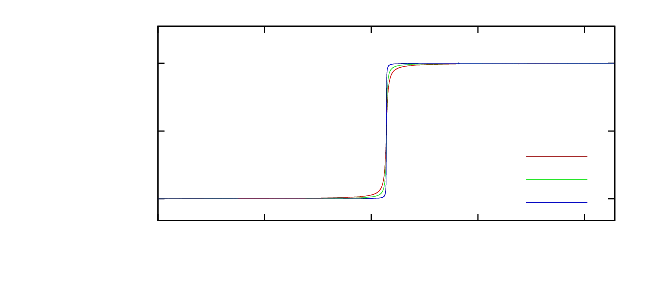
\includegraphics{sine_diff}}%
    \gplfronttext
  \end{picture}%
\endgroup

        \caption{\em Difference of the real part of the solution for
          two paths separated by a distance of $2\Delta$. Once the two
          paths pass aside of the first singularity, a step of $4\pi$
          appear. Away from the singularity, the step remains
          constant.}
        \label{fig:2d_sine_diff}
      \end{center}
    \end{figure}
    We notice that away from the singularity, the size of the step is
    essentially constant, reaching $4\pi$ for $\theta \geq
    \pi/2$. This is a consequence of Cauchy's theorem, and it is
    accurately reproduced here.
  \end{subsection}
\end{section}
\begin{section}{Application to the Vortex in $(2+1)$ dimensions}
  We now use the same procedure to compute the numerical analytic
  continuation of the Vortex, which arises in $(2+1)$ dimensional
  Yang-Mills theory with $U(1)$ gauge symmetry.
  
  The Lagrangian and the ansatz considered have been introduces in
  section \ref{sec:theory_vortex}. We now build the Cauchy problem related to the
  analytic continuation of the vortex.

  We first recast the second order differential equation system into a
  first order system: we define $B(r)=A'(r)$ and $G(r) = F'(r)$, which leads to
  \begin{align}
    \frac{\mathrm{d}}{\mathrm{d}r}A &= B(r),\\
    \frac{\mathrm{d}}{\mathrm{d}r}B &= \frac{1}{r}B(r)-2e^2 v^2F(r)^2(1-A(r)),\\
    \frac{\mathrm{d}}{\mathrm{d}r}F &= G(r),\\
    \frac{\mathrm{d}}{\mathrm{d}r}G &= -\frac{1}{r}G(r)+\lambda v^2(F(r)^2-1)F(r) +\frac{F(r)(A(r)-1)^2}{r^2}.
  \end{align}
  Promoting all the functions $A,B,F,G$ to the complex field, as well
  as $r\to z=r+iy$ and following the same procedure as previously, the
  Cauchy problem writes:
  \begin{align}
    \partial_y A_I &= B_R,\\
    -\partial_y A_R &= B_I,\\
    \partial_y B_I &= \Re\left[\frac{B_R+iB_I}{z}-2e^2v^2(F_R+iF_I)^2(1-(A_R+iA_I))\right],\\
    -\partial_y B_R &= \Im\left[\frac{B_R+iB_I}{z}-2e^2v^2(F_R+iF_I)^2(1-(A_R+iA_I))\right],\\
    \partial_y F_I &= G_R,\\
    -\partial_y F_R &= G_I,\\
    \partial_y G_I &= \Re\left[-\frac{G_R+iG_I}{z}+\lambda v^2((F_R+iF_I)^2-1)(F_R+iF_I)\right.\\
      &\hphantom{= \Re\left[-\frac{G_R+iG_I}{z}\right.}+\left.\frac{(F_R+iF_I)(A_R+iA_I-1)^2}{z^2}\right],\\
    -\partial_y G_R &= \Im\left[-\frac{G_R+iG_I}{z}+\lambda v^2((F_R+iF_I)^2-1)(F_R+iF_I)\right.\\
      &\hphantom{= \Re\left[-\frac{G_R+iG_I}{z}\right.}+\left.\frac{(F_R+iF_I)(A_R+iA_I-1)^2}{z^2}\right].\\
  \end{align}
  
  The actual computation of the real and imaginary parts of these last
  expression is clearly tedious and uninteresting. Therefore the job
  is left to the numerical implementation.

  The initial conditions of this Cauchy problem require the values of
  the the functions $A$ and $F$, as well as their derivative. Both of
  them are obtained numerically for a set of points uniformly
  distributed on the real axis, between $0$ and $R = 10$. Each of
  these points is then used as an initial condition for the analytic
  continuation.

  The initial conditions writes:
  \begin{align}
    A_R(r+i0) &= A(r),\\
    B_R(r+i0) &= \frac{\mathrm d}{\mathrm d r}A(r),\\
    F_R(r+i0) &= F(r),\\
    G_R(r+i0) &= \frac{\mathrm d}{\mathrm d r}F(r),\\
    A_I(r+i0) &= 0,\\
    B_I(r+i0) &= 0,\\
    F_I(r+i0) &= 0,\\
    G_I(r+i0) &= 0.\\
  \end{align}
  It is important to notice that the only coordinate left by the
  spherical symmetry is the radius $r$, which is not equivalent to a
  cartesian coordinate $x$ or $y$, despite the fact that they share
  the same numerical value in some situations.

  As a consequence, a path in $x$ coordinate starting at $-\infty$ and
  ending at $+\infty$ corresponds, in terms of $r$ coordinate to a path
  starting and ending at $+\infty$.

  Then, the Wick rotation of such a path brings it to the imaginary
  axis, without the need to go to the negative real half of the
  complex plane. An illustration of the Wick's rotation is shown on
  Fig. \ref{fig:s_path}.

  \begin{figure}[!ht]
    \begin{center}
      %% Creator: Inkscape inkscape 0.48.2, www.inkscape.org
%% PDF/EPS/PS + LaTeX output extension by Johan Engelen, 2010
%% Accompanies image file 'Path.pdf' (pdf, eps, ps)
%%
%% To include the image in your LaTeX document, write
%%   \input{<filename>.pdf_tex}
%%  instead of
%%   \includegraphics{<filename>.pdf}
%% To scale the image, write
%%   \def\svgwidth{<desired width>}
%%   \input{<filename>.pdf_tex}
%%  instead of
%%   \includegraphics[width=<desired width>]{<filename>.pdf}
%%
%% Images with a different path to the parent latex file can
%% be accessed with the `import' package (which may need to be
%% installed) using
%%   \usepackage{import}
%% in the preamble, and then including the image with
%%   \import{<path to file>}{<filename>.pdf_tex}
%% Alternatively, one can specify
%%   \graphicspath{{<path to file>/}}
%% 
%% For more information, please see info/svg-inkscape on CTAN:
%%   http://tug.ctan.org/tex-archive/info/svg-inkscape
%%
\begingroup%
  \makeatletter%
  \providecommand\color[2][]{%
    \errmessage{(Inkscape) Color is used for the text in Inkscape, but the package 'color.sty' is not loaded}%
    \renewcommand\color[2][]{}%
  }%
  \providecommand\transparent[1]{%
    \errmessage{(Inkscape) Transparency is used (non-zero) for the text in Inkscape, but the package 'transparent.sty' is not loaded}%
    \renewcommand\transparent[1]{}%
  }%
  \providecommand\rotatebox[2]{#2}%
  \ifx\svgwidth\undefined%
    \setlength{\unitlength}{311.81101074bp}%
    \ifx\svgscale\undefined%
      \relax%
    \else%
      \setlength{\unitlength}{\unitlength * \real{\svgscale}}%
    \fi%
  \else%
    \setlength{\unitlength}{\svgwidth}%
  \fi%
  \global\let\svgwidth\undefined%
  \global\let\svgscale\undefined%
  \makeatother%
  \begin{picture}(1,0.45454545)%
    \put(0,0){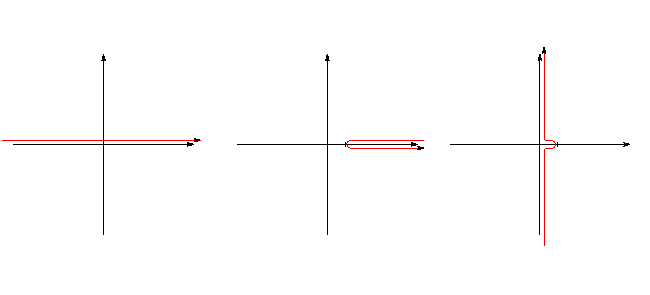
\includegraphics[width=\unitlength]{path.pdf}}%
    \put(0.17043291,0.34819635){\color[rgb]{0,0,0}\makebox(0,0)[lb]{\smash{{\scriptsize $y$}}}}%
    \put(0.26206351,0.20341996){\color[rgb]{0,0,0}\makebox(0,0)[lb]{\smash{{\scriptsize $x$}}}}%
    \put(0.60659455,0.19975469){\color[rgb]{0,0,0}\makebox(0,0)[lb]{\smash{{\scriptsize $r$}}}}%
    \put(0.94196251,0.20158733){\color[rgb]{0,0,0}\makebox(0,0)[lb]{\smash{{\scriptsize $r$}}}}%
    \put(0.84483407,0.35369409){\color[rgb]{0,0,0}\makebox(0,0)[lb]{\smash{{\scriptsize $t$}}}}%
  \end{picture}%
\endgroup%

      \caption{\em The choice of the radius $r$ as the coordinate has
        implications on the Wick rotation of the integration path in
        the complex plane. The path starting from $-\infty$ to
        $+\infty$ for the cartesian coordinate $x$ is wrapped in
        $r$-space on $\mathbb{R}_+$. The Wick rotation then bring the
        wrapped path to the imaginary axis, without the need to go to the
        negative imaginary half plane.}
      \label{fig:s_path}
    \end{center}
  \end{figure}
  
  It is therefore sufficient to restrict the computation of the
  analytic continuation to the positive real half of the complex
  plane. We only integrate a little further to make the localization
  of the singularities easier.

  We have computed the analytic continuation of the vortex only in
  the BPS limit case ($\lambda = 1$). The result for the real and
  imaginary parts of functions $A(z)$ and $F(z)$ is shown on
  Fig. \ref{fig:cm_vortex_a_real}--\ref{fig:cm_vortex_f_imag}.
  \begin{subsection}{Numerical analytic continuation in the BPS limit}
    \begin{figure}[!ht]
      \begin{center}
        % GNUPLOT: LaTeX picture with Postscript
\begingroup
\scriptsize
  \makeatletter
  \providecommand\color[2][]{%
    \GenericError{(gnuplot) \space\space\space\@spaces}{%
      Package color not loaded in conjunction with
      terminal option `colourtext'%
    }{See the gnuplot documentation for explanation.%
    }{Either use 'blacktext' in gnuplot or load the package
      color.sty in LaTeX.}%
    \renewcommand\color[2][]{}%
  }%
  \providecommand\includegraphics[2][]{%
    \GenericError{(gnuplot) \space\space\space\@spaces}{%
      Package graphicx or graphics not loaded%
    }{See the gnuplot documentation for explanation.%
    }{The gnuplot epslatex terminal needs graphicx.sty or graphics.sty.}%
    \renewcommand\includegraphics[2][]{}%
  }%
  \providecommand\rotatebox[2]{#2}%
  \@ifundefined{ifGPcolor}{%
    \newif\ifGPcolor
    \GPcolortrue
  }{}%
  \@ifundefined{ifGPblacktext}{%
    \newif\ifGPblacktext
    \GPblacktexttrue
  }{}%
  % define a \g@addto@macro without @ in the name:
  \let\gplgaddtomacro\g@addto@macro
  % define empty templates for all commands taking text:
  \gdef\gplbacktext{}%
  \gdef\gplfronttext{}%
  \makeatother
  \ifGPblacktext
    % no textcolor at all
    \def\colorrgb#1{}%
    \def\colorgray#1{}%
  \else
    % gray or color?
    \ifGPcolor
      \def\colorrgb#1{\color[rgb]{#1}}%
      \def\colorgray#1{\color[gray]{#1}}%
      \expandafter\def\csname LTw\endcsname{\color{white}}%
      \expandafter\def\csname LTb\endcsname{\color{black}}%
      \expandafter\def\csname LTa\endcsname{\color{black}}%
      \expandafter\def\csname LT0\endcsname{\color[rgb]{1,0,0}}%
      \expandafter\def\csname LT1\endcsname{\color[rgb]{0,1,0}}%
      \expandafter\def\csname LT2\endcsname{\color[rgb]{0,0,1}}%
      \expandafter\def\csname LT3\endcsname{\color[rgb]{1,0,1}}%
      \expandafter\def\csname LT4\endcsname{\color[rgb]{0,1,1}}%
      \expandafter\def\csname LT5\endcsname{\color[rgb]{1,1,0}}%
      \expandafter\def\csname LT6\endcsname{\color[rgb]{0,0,0}}%
      \expandafter\def\csname LT7\endcsname{\color[rgb]{1,0.3,0}}%
      \expandafter\def\csname LT8\endcsname{\color[rgb]{0.5,0.5,0.5}}%
    \else
      % gray
      \def\colorrgb#1{\color{black}}%
      \def\colorgray#1{\color[gray]{#1}}%
      \expandafter\def\csname LTw\endcsname{\color{white}}%
      \expandafter\def\csname LTb\endcsname{\color{black}}%
      \expandafter\def\csname LTa\endcsname{\color{black}}%
      \expandafter\def\csname LT0\endcsname{\color{black}}%
      \expandafter\def\csname LT1\endcsname{\color{black}}%
      \expandafter\def\csname LT2\endcsname{\color{black}}%
      \expandafter\def\csname LT3\endcsname{\color{black}}%
      \expandafter\def\csname LT4\endcsname{\color{black}}%
      \expandafter\def\csname LT5\endcsname{\color{black}}%
      \expandafter\def\csname LT6\endcsname{\color{black}}%
      \expandafter\def\csname LT7\endcsname{\color{black}}%
      \expandafter\def\csname LT8\endcsname{\color{black}}%
    \fi
  \fi
  \setlength{\unitlength}{0.0500bp}%
  \begin{picture}(6236.00,2834.00)%
    \gplgaddtomacro\gplbacktext{%
    }%
    \gplgaddtomacro\gplfronttext{%
      \csname LTb\endcsname%
      \put(1046,517){\makebox(0,0){\strut{}-10}}%
      \put(2082,517){\makebox(0,0){\strut{}-5}}%
      \put(3118,517){\makebox(0,0){\strut{} 0}}%
      \put(4154,517){\makebox(0,0){\strut{} 5}}%
      \put(5190,517){\makebox(0,0){\strut{} 10}}%
      \put(3118,187){\makebox(0,0){\strut{}$x$}}%
      \put(874,803){\makebox(0,0)[r]{\strut{} 0}}%
      \put(874,1527){\makebox(0,0)[r]{\strut{} 5}}%
      \put(874,2251){\makebox(0,0)[r]{\strut{} 10}}%
      \put(544,1527){\rotatebox{-270}{\makebox(0,0){\strut{}$y$}}}%
      \put(5633,816){\makebox(0,0)[l]{\strut{}-5}}%
      \put(5633,1526){\makebox(0,0)[l]{\strut{} 0}}%
      \put(5633,2236){\makebox(0,0)[l]{\strut{} 5}}%
    }%
    \gplbacktext
    \put(0,0){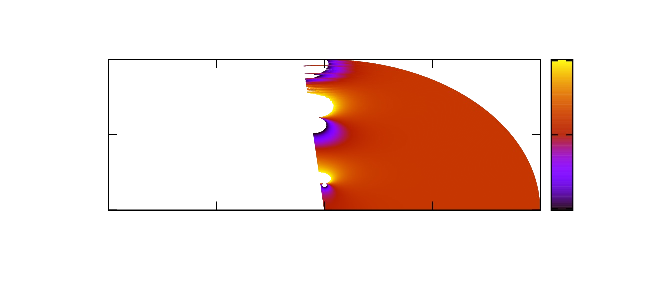
\includegraphics{vortex_anal_a_real}}%
    \gplfronttext
  \end{picture}%
\endgroup

        \caption{\em Real part of the function $A(z)$. The function is
          even under conjugation: $\Re A(z) = \Re A(\bar z)$. The
          singularity which is closest to the origin is on the
          imaginary axis ($z_0 \approx 0+1.78i$). The second one is
          slightly shifted to the negative real half plane
          ($z_0\approx -0.4+6.1i$). }
        \label{fig:cm_vortex_a_real}
      \end{center}
    \end{figure}

    \begin{figure}[!ht]
      \begin{center}
        % GNUPLOT: LaTeX picture with Postscript
\begingroup
\scriptsize
  \makeatletter
  \providecommand\color[2][]{%
    \GenericError{(gnuplot) \space\space\space\@spaces}{%
      Package color not loaded in conjunction with
      terminal option `colourtext'%
    }{See the gnuplot documentation for explanation.%
    }{Either use 'blacktext' in gnuplot or load the package
      color.sty in LaTeX.}%
    \renewcommand\color[2][]{}%
  }%
  \providecommand\includegraphics[2][]{%
    \GenericError{(gnuplot) \space\space\space\@spaces}{%
      Package graphicx or graphics not loaded%
    }{See the gnuplot documentation for explanation.%
    }{The gnuplot epslatex terminal needs graphicx.sty or graphics.sty.}%
    \renewcommand\includegraphics[2][]{}%
  }%
  \providecommand\rotatebox[2]{#2}%
  \@ifundefined{ifGPcolor}{%
    \newif\ifGPcolor
    \GPcolortrue
  }{}%
  \@ifundefined{ifGPblacktext}{%
    \newif\ifGPblacktext
    \GPblacktexttrue
  }{}%
  % define a \g@addto@macro without @ in the name:
  \let\gplgaddtomacro\g@addto@macro
  % define empty templates for all commands taking text:
  \gdef\gplbacktext{}%
  \gdef\gplfronttext{}%
  \makeatother
  \ifGPblacktext
    % no textcolor at all
    \def\colorrgb#1{}%
    \def\colorgray#1{}%
  \else
    % gray or color?
    \ifGPcolor
      \def\colorrgb#1{\color[rgb]{#1}}%
      \def\colorgray#1{\color[gray]{#1}}%
      \expandafter\def\csname LTw\endcsname{\color{white}}%
      \expandafter\def\csname LTb\endcsname{\color{black}}%
      \expandafter\def\csname LTa\endcsname{\color{black}}%
      \expandafter\def\csname LT0\endcsname{\color[rgb]{1,0,0}}%
      \expandafter\def\csname LT1\endcsname{\color[rgb]{0,1,0}}%
      \expandafter\def\csname LT2\endcsname{\color[rgb]{0,0,1}}%
      \expandafter\def\csname LT3\endcsname{\color[rgb]{1,0,1}}%
      \expandafter\def\csname LT4\endcsname{\color[rgb]{0,1,1}}%
      \expandafter\def\csname LT5\endcsname{\color[rgb]{1,1,0}}%
      \expandafter\def\csname LT6\endcsname{\color[rgb]{0,0,0}}%
      \expandafter\def\csname LT7\endcsname{\color[rgb]{1,0.3,0}}%
      \expandafter\def\csname LT8\endcsname{\color[rgb]{0.5,0.5,0.5}}%
    \else
      % gray
      \def\colorrgb#1{\color{black}}%
      \def\colorgray#1{\color[gray]{#1}}%
      \expandafter\def\csname LTw\endcsname{\color{white}}%
      \expandafter\def\csname LTb\endcsname{\color{black}}%
      \expandafter\def\csname LTa\endcsname{\color{black}}%
      \expandafter\def\csname LT0\endcsname{\color{black}}%
      \expandafter\def\csname LT1\endcsname{\color{black}}%
      \expandafter\def\csname LT2\endcsname{\color{black}}%
      \expandafter\def\csname LT3\endcsname{\color{black}}%
      \expandafter\def\csname LT4\endcsname{\color{black}}%
      \expandafter\def\csname LT5\endcsname{\color{black}}%
      \expandafter\def\csname LT6\endcsname{\color{black}}%
      \expandafter\def\csname LT7\endcsname{\color{black}}%
      \expandafter\def\csname LT8\endcsname{\color{black}}%
    \fi
  \fi
  \setlength{\unitlength}{0.0500bp}%
  \begin{picture}(6236.00,2834.00)%
    \gplgaddtomacro\gplbacktext{%
    }%
    \gplgaddtomacro\gplfronttext{%
      \csname LTb\endcsname%
      \put(1046,517){\makebox(0,0){\strut{}-10}}%
      \put(2082,517){\makebox(0,0){\strut{}-5}}%
      \put(3118,517){\makebox(0,0){\strut{} 0}}%
      \put(4154,517){\makebox(0,0){\strut{} 5}}%
      \put(5190,517){\makebox(0,0){\strut{} 10}}%
      \put(3118,187){\makebox(0,0){\strut{}$x$}}%
      \put(874,803){\makebox(0,0)[r]{\strut{} 0}}%
      \put(874,1527){\makebox(0,0)[r]{\strut{} 5}}%
      \put(874,2251){\makebox(0,0)[r]{\strut{} 10}}%
      \put(544,1527){\rotatebox{-270}{\makebox(0,0){\strut{}$y$}}}%
      \put(5633,836){\makebox(0,0)[l]{\strut{}-2}}%
      \put(5633,1526){\makebox(0,0)[l]{\strut{} 0}}%
      \put(5633,2216){\makebox(0,0)[l]{\strut{} 2}}%
    }%
    \gplbacktext
    \put(0,0){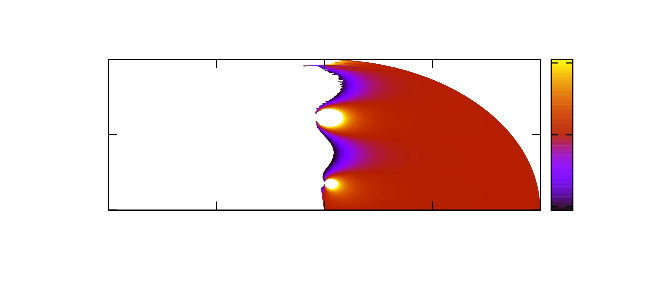
\includegraphics{vortex_anal_a_imag}}%
    \gplfronttext
  \end{picture}%
\endgroup

        \caption{\em Imaginary part of the function $A(z)$. The function is
          odd under conjugation: $\Im A(z) = -\Im A(\bar z)$.}
        \label{fig:cm_vortex_a_imag}
      \end{center}
    \end{figure}

    \begin{figure}[!ht]
      \begin{center}
        % GNUPLOT: LaTeX picture with Postscript
\begingroup
\scriptsize
  \makeatletter
  \providecommand\color[2][]{%
    \GenericError{(gnuplot) \space\space\space\@spaces}{%
      Package color not loaded in conjunction with
      terminal option `colourtext'%
    }{See the gnuplot documentation for explanation.%
    }{Either use 'blacktext' in gnuplot or load the package
      color.sty in LaTeX.}%
    \renewcommand\color[2][]{}%
  }%
  \providecommand\includegraphics[2][]{%
    \GenericError{(gnuplot) \space\space\space\@spaces}{%
      Package graphicx or graphics not loaded%
    }{See the gnuplot documentation for explanation.%
    }{The gnuplot epslatex terminal needs graphicx.sty or graphics.sty.}%
    \renewcommand\includegraphics[2][]{}%
  }%
  \providecommand\rotatebox[2]{#2}%
  \@ifundefined{ifGPcolor}{%
    \newif\ifGPcolor
    \GPcolortrue
  }{}%
  \@ifundefined{ifGPblacktext}{%
    \newif\ifGPblacktext
    \GPblacktexttrue
  }{}%
  % define a \g@addto@macro without @ in the name:
  \let\gplgaddtomacro\g@addto@macro
  % define empty templates for all commands taking text:
  \gdef\gplbacktext{}%
  \gdef\gplfronttext{}%
  \makeatother
  \ifGPblacktext
    % no textcolor at all
    \def\colorrgb#1{}%
    \def\colorgray#1{}%
  \else
    % gray or color?
    \ifGPcolor
      \def\colorrgb#1{\color[rgb]{#1}}%
      \def\colorgray#1{\color[gray]{#1}}%
      \expandafter\def\csname LTw\endcsname{\color{white}}%
      \expandafter\def\csname LTb\endcsname{\color{black}}%
      \expandafter\def\csname LTa\endcsname{\color{black}}%
      \expandafter\def\csname LT0\endcsname{\color[rgb]{1,0,0}}%
      \expandafter\def\csname LT1\endcsname{\color[rgb]{0,1,0}}%
      \expandafter\def\csname LT2\endcsname{\color[rgb]{0,0,1}}%
      \expandafter\def\csname LT3\endcsname{\color[rgb]{1,0,1}}%
      \expandafter\def\csname LT4\endcsname{\color[rgb]{0,1,1}}%
      \expandafter\def\csname LT5\endcsname{\color[rgb]{1,1,0}}%
      \expandafter\def\csname LT6\endcsname{\color[rgb]{0,0,0}}%
      \expandafter\def\csname LT7\endcsname{\color[rgb]{1,0.3,0}}%
      \expandafter\def\csname LT8\endcsname{\color[rgb]{0.5,0.5,0.5}}%
    \else
      % gray
      \def\colorrgb#1{\color{black}}%
      \def\colorgray#1{\color[gray]{#1}}%
      \expandafter\def\csname LTw\endcsname{\color{white}}%
      \expandafter\def\csname LTb\endcsname{\color{black}}%
      \expandafter\def\csname LTa\endcsname{\color{black}}%
      \expandafter\def\csname LT0\endcsname{\color{black}}%
      \expandafter\def\csname LT1\endcsname{\color{black}}%
      \expandafter\def\csname LT2\endcsname{\color{black}}%
      \expandafter\def\csname LT3\endcsname{\color{black}}%
      \expandafter\def\csname LT4\endcsname{\color{black}}%
      \expandafter\def\csname LT5\endcsname{\color{black}}%
      \expandafter\def\csname LT6\endcsname{\color{black}}%
      \expandafter\def\csname LT7\endcsname{\color{black}}%
      \expandafter\def\csname LT8\endcsname{\color{black}}%
    \fi
  \fi
  \setlength{\unitlength}{0.0500bp}%
  \begin{picture}(6236.00,2834.00)%
    \gplgaddtomacro\gplbacktext{%
    }%
    \gplgaddtomacro\gplfronttext{%
      \csname LTb\endcsname%
      \put(1046,517){\makebox(0,0){\strut{}-10}}%
      \put(2082,517){\makebox(0,0){\strut{}-5}}%
      \put(3118,517){\makebox(0,0){\strut{} 0}}%
      \put(4154,517){\makebox(0,0){\strut{} 5}}%
      \put(5190,517){\makebox(0,0){\strut{} 10}}%
      \put(3118,187){\makebox(0,0){\strut{}$x$}}%
      \put(874,803){\makebox(0,0)[r]{\strut{} 0}}%
      \put(874,1527){\makebox(0,0)[r]{\strut{} 5}}%
      \put(874,2251){\makebox(0,0)[r]{\strut{} 10}}%
      \put(544,1527){\rotatebox{-270}{\makebox(0,0){\strut{}$y$}}}%
      \put(5633,836){\makebox(0,0)[l]{\strut{}-2}}%
      \put(5633,1526){\makebox(0,0)[l]{\strut{} 0}}%
      \put(5633,2216){\makebox(0,0)[l]{\strut{} 2}}%
    }%
    \gplbacktext
    \put(0,0){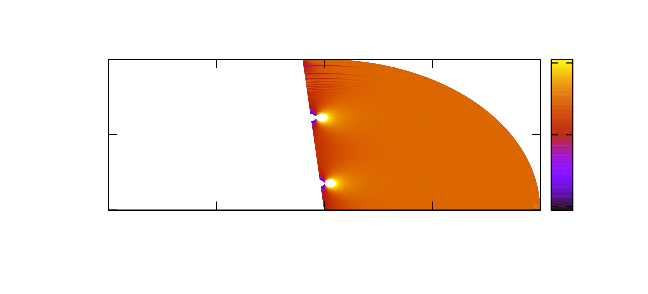
\includegraphics{vortex_anal_f_real}}%
    \gplfronttext
  \end{picture}%
\endgroup

        \caption{\em Real part of the function $F(z)$. The function is
          even under conjugation: $\Re F(z) = \Re F(\bar z)$. The
          locations of the singularities are the same as for the
          function $A(z)$.}
        \label{fig:cm_vortex_f_real}
      \end{center}
    \end{figure}

    \begin{figure}[!ht]
      \begin{center}
        % GNUPLOT: LaTeX picture with Postscript
\begingroup
\scriptsize
  \makeatletter
  \providecommand\color[2][]{%
    \GenericError{(gnuplot) \space\space\space\@spaces}{%
      Package color not loaded in conjunction with
      terminal option `colourtext'%
    }{See the gnuplot documentation for explanation.%
    }{Either use 'blacktext' in gnuplot or load the package
      color.sty in LaTeX.}%
    \renewcommand\color[2][]{}%
  }%
  \providecommand\includegraphics[2][]{%
    \GenericError{(gnuplot) \space\space\space\@spaces}{%
      Package graphicx or graphics not loaded%
    }{See the gnuplot documentation for explanation.%
    }{The gnuplot epslatex terminal needs graphicx.sty or graphics.sty.}%
    \renewcommand\includegraphics[2][]{}%
  }%
  \providecommand\rotatebox[2]{#2}%
  \@ifundefined{ifGPcolor}{%
    \newif\ifGPcolor
    \GPcolortrue
  }{}%
  \@ifundefined{ifGPblacktext}{%
    \newif\ifGPblacktext
    \GPblacktexttrue
  }{}%
  % define a \g@addto@macro without @ in the name:
  \let\gplgaddtomacro\g@addto@macro
  % define empty templates for all commands taking text:
  \gdef\gplbacktext{}%
  \gdef\gplfronttext{}%
  \makeatother
  \ifGPblacktext
    % no textcolor at all
    \def\colorrgb#1{}%
    \def\colorgray#1{}%
  \else
    % gray or color?
    \ifGPcolor
      \def\colorrgb#1{\color[rgb]{#1}}%
      \def\colorgray#1{\color[gray]{#1}}%
      \expandafter\def\csname LTw\endcsname{\color{white}}%
      \expandafter\def\csname LTb\endcsname{\color{black}}%
      \expandafter\def\csname LTa\endcsname{\color{black}}%
      \expandafter\def\csname LT0\endcsname{\color[rgb]{1,0,0}}%
      \expandafter\def\csname LT1\endcsname{\color[rgb]{0,1,0}}%
      \expandafter\def\csname LT2\endcsname{\color[rgb]{0,0,1}}%
      \expandafter\def\csname LT3\endcsname{\color[rgb]{1,0,1}}%
      \expandafter\def\csname LT4\endcsname{\color[rgb]{0,1,1}}%
      \expandafter\def\csname LT5\endcsname{\color[rgb]{1,1,0}}%
      \expandafter\def\csname LT6\endcsname{\color[rgb]{0,0,0}}%
      \expandafter\def\csname LT7\endcsname{\color[rgb]{1,0.3,0}}%
      \expandafter\def\csname LT8\endcsname{\color[rgb]{0.5,0.5,0.5}}%
    \else
      % gray
      \def\colorrgb#1{\color{black}}%
      \def\colorgray#1{\color[gray]{#1}}%
      \expandafter\def\csname LTw\endcsname{\color{white}}%
      \expandafter\def\csname LTb\endcsname{\color{black}}%
      \expandafter\def\csname LTa\endcsname{\color{black}}%
      \expandafter\def\csname LT0\endcsname{\color{black}}%
      \expandafter\def\csname LT1\endcsname{\color{black}}%
      \expandafter\def\csname LT2\endcsname{\color{black}}%
      \expandafter\def\csname LT3\endcsname{\color{black}}%
      \expandafter\def\csname LT4\endcsname{\color{black}}%
      \expandafter\def\csname LT5\endcsname{\color{black}}%
      \expandafter\def\csname LT6\endcsname{\color{black}}%
      \expandafter\def\csname LT7\endcsname{\color{black}}%
      \expandafter\def\csname LT8\endcsname{\color{black}}%
    \fi
  \fi
  \setlength{\unitlength}{0.0500bp}%
  \begin{picture}(6236.00,2834.00)%
    \gplgaddtomacro\gplbacktext{%
    }%
    \gplgaddtomacro\gplfronttext{%
      \csname LTb\endcsname%
      \put(1046,517){\makebox(0,0){\strut{}-10}}%
      \put(2082,517){\makebox(0,0){\strut{}-5}}%
      \put(3118,517){\makebox(0,0){\strut{} 0}}%
      \put(4154,517){\makebox(0,0){\strut{} 5}}%
      \put(5190,517){\makebox(0,0){\strut{} 10}}%
      \put(3118,187){\makebox(0,0){\strut{}$x$}}%
      \put(874,803){\makebox(0,0)[r]{\strut{} 0}}%
      \put(874,1527){\makebox(0,0)[r]{\strut{} 5}}%
      \put(874,2251){\makebox(0,0)[r]{\strut{} 10}}%
      \put(544,1527){\rotatebox{-270}{\makebox(0,0){\strut{}$y$}}}%
      \put(5633,816){\makebox(0,0)[l]{\strut{}-5}}%
      \put(5633,1526){\makebox(0,0)[l]{\strut{} 0}}%
      \put(5633,2236){\makebox(0,0)[l]{\strut{} 5}}%
    }%
    \gplbacktext
    \put(0,0){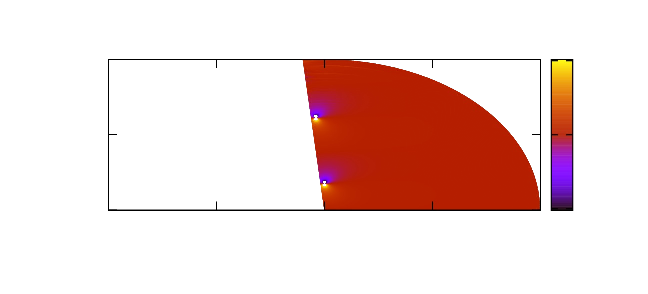
\includegraphics{vortex_anal_f_imag}}%
    \gplfronttext
  \end{picture}%
\endgroup

        \caption{\em Imaginary part of the function $F(z)$. The function is
          odd under conjugation: $\Im F(z) = -\Im F(\bar z)$.}
        \label{fig:cm_vortex_f_imag}
      \end{center}
    \end{figure}
    We notice two singularities. The first, which is the closest to
    the origin, lies on the imaginary axis, at least at machine
    precision. However, the next singularity is off the imaginary
    axis, and is located on the second quadrant.
    
    The important point is that in positive half of the complex plane,
    and within the range considered, the analytic continuation of
    the vortex solution do not show any singularities. This is
    comforting, since it means that the Wick rotation should be valid
    and doable in principle.
  \end{subsection}
  \begin{subsection}{Analytic study of the convergence of the Taylor Series}
    We have now some clues about the existence of a singularity on the
    imaginary axis. But numerical results are difficult to interpret,
    and it would be nice to have an analytic approach to validate
    this statement.
    
    The idea is to find the Taylor series for the two functions around
    $z = 0$, and then extract the radius of convergence of these
    series.
    
    Let $N$ be the order of the Taylor expansions. Using the
    asymptotics of the two functions $A$ and $F$, we may write:
    \begin{align}
      A(z) = \alpha z^2 + \sum_{i=3}^N a_iz^i +O(z^{N+1}),\\
      F(z) = \beta z+ \sum_{i=2}^N f_iz^i +O(z^{N+1}).
    \end{align}
    We then substitute these expression into the system of differential
    equations (\ref{eq:vortex_1})--(\ref{eq:vortex_2}). These equations
    must be satisfied at each order in $z$. Each coefficient of powers
    of $z$ must cancel, providing a set of equations. $\alpha$ and
    $\beta$ are two free parameters which correspond to the two
    additional initial conditions required to solve a system of 2 second
    order differential equations. These can be extracted from the
    numerical approximation of the vortex.
    
    The set of equations has been solved with the help of
    Mathematica. An estimation of the radius of convergence is
    presented on Fig. \ref{fig:coeff}.
    \begin{figure}[ht!]
      \begin{center}
        % GNUPLOT: LaTeX picture with Postscript
\begingroup
  \makeatletter
  \providecommand\color[2][]{%
    \GenericError{(gnuplot) \space\space\space\@spaces}{%
      Package color not loaded in conjunction with
      terminal option `colourtext'%
    }{See the gnuplot documentation for explanation.%
    }{Either use 'blacktext' in gnuplot or load the package
      color.sty in LaTeX.}%
    \renewcommand\color[2][]{}%
  }%
  \providecommand\includegraphics[2][]{%
    \GenericError{(gnuplot) \space\space\space\@spaces}{%
      Package graphicx or graphics not loaded%
    }{See the gnuplot documentation for explanation.%
    }{The gnuplot epslatex terminal needs graphicx.sty or graphics.sty.}%
    \renewcommand\includegraphics[2][]{}%
  }%
  \providecommand\rotatebox[2]{#2}%
  \@ifundefined{ifGPcolor}{%
    \newif\ifGPcolor
    \GPcolortrue
  }{}%
  \@ifundefined{ifGPblacktext}{%
    \newif\ifGPblacktext
    \GPblacktexttrue
  }{}%
  % define a \g@addto@macro without @ in the name:
  \let\gplgaddtomacro\g@addto@macro
  % define empty templates for all commands taking text:
  \gdef\gplbacktext{}%
  \gdef\gplfronttext{}%
  \makeatother
  \ifGPblacktext
    % no textcolor at all
    \def\colorrgb#1{}%
    \def\colorgray#1{}%
  \else
    % gray or color?
    \ifGPcolor
      \def\colorrgb#1{\color[rgb]{#1}}%
      \def\colorgray#1{\color[gray]{#1}}%
      \expandafter\def\csname LTw\endcsname{\color{white}}%
      \expandafter\def\csname LTb\endcsname{\color{black}}%
      \expandafter\def\csname LTa\endcsname{\color{black}}%
      \expandafter\def\csname LT0\endcsname{\color[rgb]{1,0,0}}%
      \expandafter\def\csname LT1\endcsname{\color[rgb]{0,1,0}}%
      \expandafter\def\csname LT2\endcsname{\color[rgb]{0,0,1}}%
      \expandafter\def\csname LT3\endcsname{\color[rgb]{1,0,1}}%
      \expandafter\def\csname LT4\endcsname{\color[rgb]{0,1,1}}%
      \expandafter\def\csname LT5\endcsname{\color[rgb]{1,1,0}}%
      \expandafter\def\csname LT6\endcsname{\color[rgb]{0,0,0}}%
      \expandafter\def\csname LT7\endcsname{\color[rgb]{1,0.3,0}}%
      \expandafter\def\csname LT8\endcsname{\color[rgb]{0.5,0.5,0.5}}%
    \else
      % gray
      \def\colorrgb#1{\color{black}}%
      \def\colorgray#1{\color[gray]{#1}}%
      \expandafter\def\csname LTw\endcsname{\color{white}}%
      \expandafter\def\csname LTb\endcsname{\color{black}}%
      \expandafter\def\csname LTa\endcsname{\color{black}}%
      \expandafter\def\csname LT0\endcsname{\color{black}}%
      \expandafter\def\csname LT1\endcsname{\color{black}}%
      \expandafter\def\csname LT2\endcsname{\color{black}}%
      \expandafter\def\csname LT3\endcsname{\color{black}}%
      \expandafter\def\csname LT4\endcsname{\color{black}}%
      \expandafter\def\csname LT5\endcsname{\color{black}}%
      \expandafter\def\csname LT6\endcsname{\color{black}}%
      \expandafter\def\csname LT7\endcsname{\color{black}}%
      \expandafter\def\csname LT8\endcsname{\color{black}}%
    \fi
  \fi
  \setlength{\unitlength}{0.0500bp}%
  \begin{picture}(6236.00,2550.00)%
    \gplgaddtomacro\gplbacktext{%
      \csname LTb\endcsname%
      \put(1078,704){\makebox(0,0)[r]{\strut{} 1.75}}%
      \put(1078,880){\makebox(0,0)[r]{\strut{} 1.8}}%
      \put(1078,1055){\makebox(0,0)[r]{\strut{} 1.85}}%
      \put(1078,1231){\makebox(0,0)[r]{\strut{} 1.9}}%
      \put(1078,1407){\makebox(0,0)[r]{\strut{} 1.95}}%
      \put(1078,1582){\makebox(0,0)[r]{\strut{} 2}}%
      \put(1078,1758){\makebox(0,0)[r]{\strut{} 2.05}}%
      \put(1078,1934){\makebox(0,0)[r]{\strut{} 2.1}}%
      \put(1078,2109){\makebox(0,0)[r]{\strut{} 2.15}}%
      \put(1078,2285){\makebox(0,0)[r]{\strut{} 2.2}}%
      \put(1210,484){\makebox(0,0){\strut{} 0}}%
      \put(1789,484){\makebox(0,0){\strut{} 5}}%
      \put(2367,484){\makebox(0,0){\strut{} 10}}%
      \put(2946,484){\makebox(0,0){\strut{} 15}}%
      \put(3525,484){\makebox(0,0){\strut{} 20}}%
      \put(4103,484){\makebox(0,0){\strut{} 25}}%
      \put(4682,484){\makebox(0,0){\strut{} 30}}%
      \put(5260,484){\makebox(0,0){\strut{} 35}}%
      \put(5839,484){\makebox(0,0){\strut{} 40}}%
      \put(176,1494){\rotatebox{-270}{\makebox(0,0){\strut{}$1/\sqrt[i]{|a_i|}$}}}%
      \put(3524,154){\makebox(0,0){\strut{}$i$}}%
    }%
    \gplgaddtomacro\gplfronttext{%
    }%
    \gplbacktext
    \put(0,0){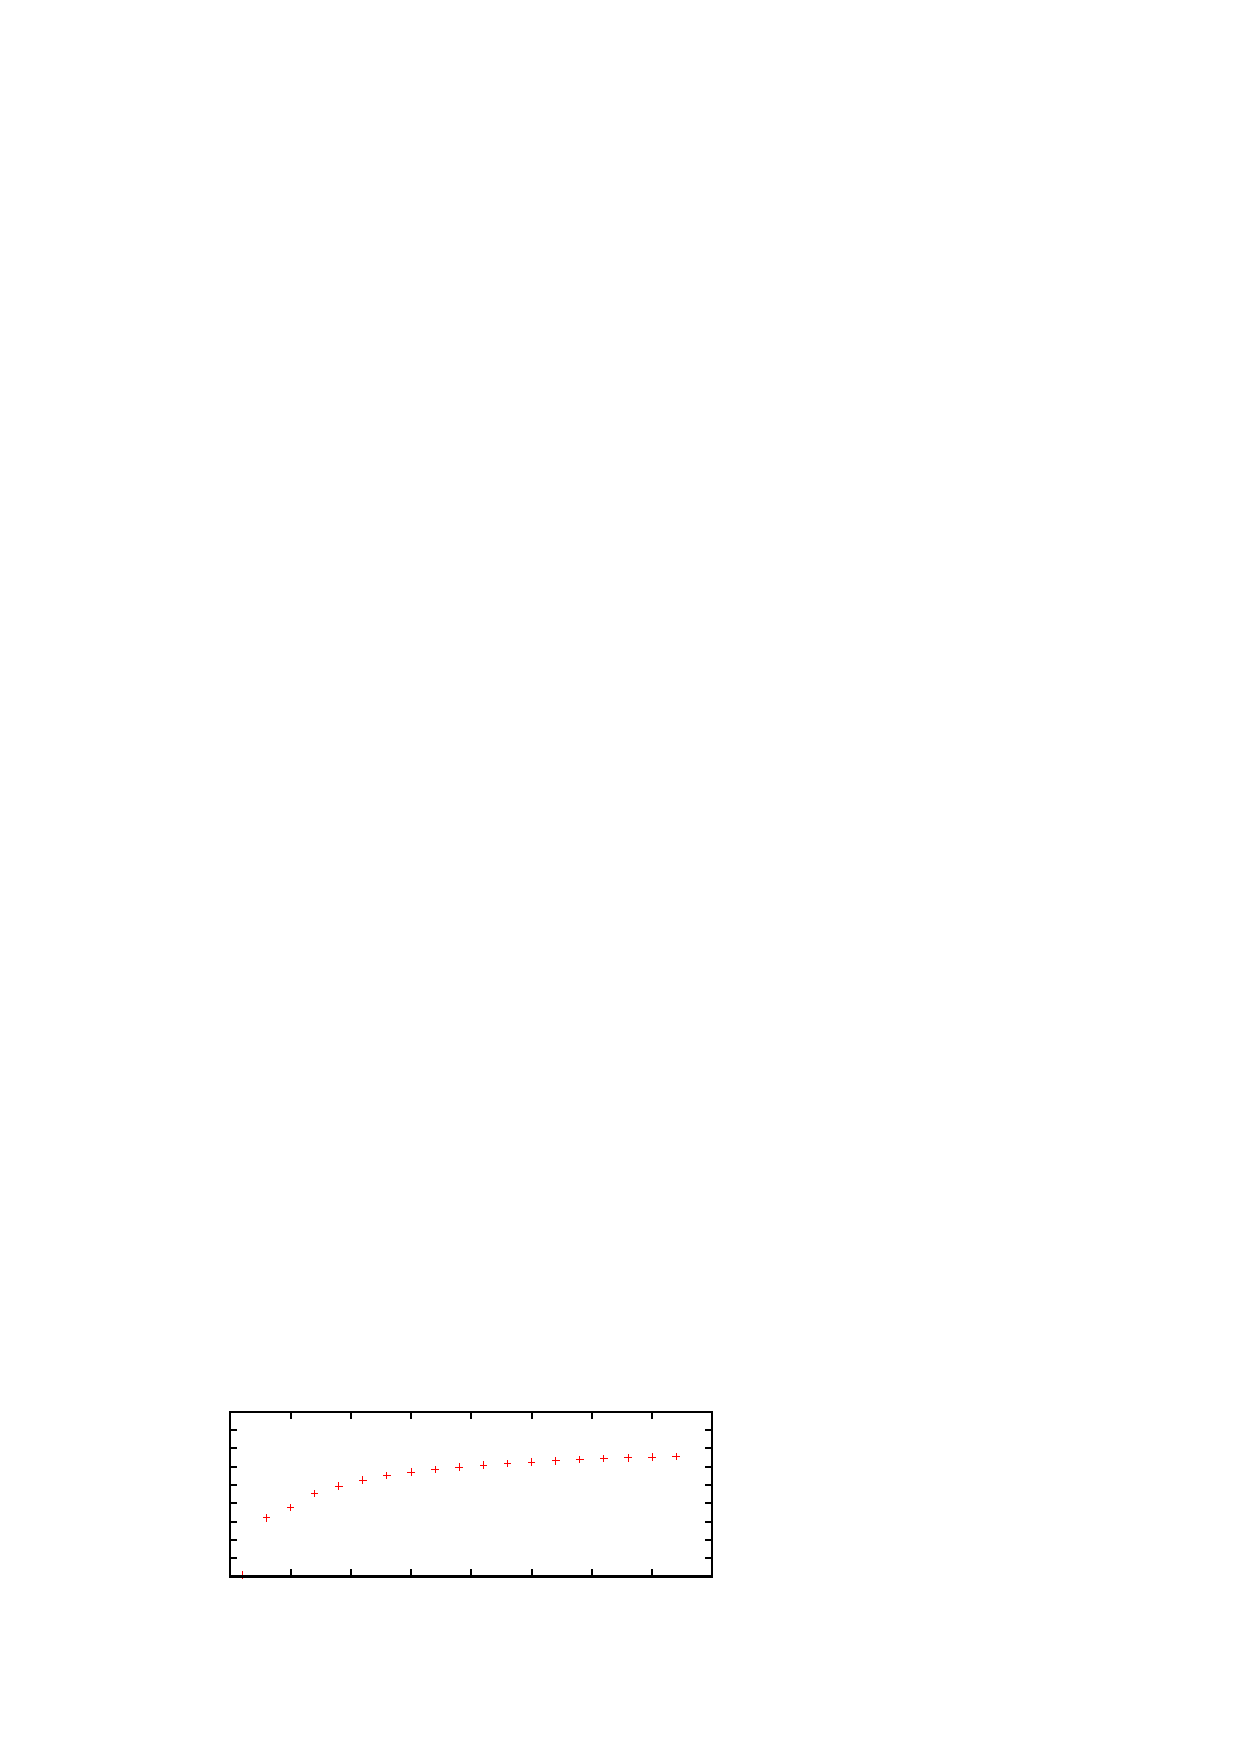
\includegraphics{laurent_a}}%
    \gplfronttext
  \end{picture}%
\endgroup

        % GNUPLOT: LaTeX picture with Postscript
\begingroup
  \makeatletter
  \providecommand\color[2][]{%
    \GenericError{(gnuplot) \space\space\space\@spaces}{%
      Package color not loaded in conjunction with
      terminal option `colourtext'%
    }{See the gnuplot documentation for explanation.%
    }{Either use 'blacktext' in gnuplot or load the package
      color.sty in LaTeX.}%
    \renewcommand\color[2][]{}%
  }%
  \providecommand\includegraphics[2][]{%
    \GenericError{(gnuplot) \space\space\space\@spaces}{%
      Package graphicx or graphics not loaded%
    }{See the gnuplot documentation for explanation.%
    }{The gnuplot epslatex terminal needs graphicx.sty or graphics.sty.}%
    \renewcommand\includegraphics[2][]{}%
  }%
  \providecommand\rotatebox[2]{#2}%
  \@ifundefined{ifGPcolor}{%
    \newif\ifGPcolor
    \GPcolortrue
  }{}%
  \@ifundefined{ifGPblacktext}{%
    \newif\ifGPblacktext
    \GPblacktexttrue
  }{}%
  % define a \g@addto@macro without @ in the name:
  \let\gplgaddtomacro\g@addto@macro
  % define empty templates for all commands taking text:
  \gdef\gplbacktext{}%
  \gdef\gplfronttext{}%
  \makeatother
  \ifGPblacktext
    % no textcolor at all
    \def\colorrgb#1{}%
    \def\colorgray#1{}%
  \else
    % gray or color?
    \ifGPcolor
      \def\colorrgb#1{\color[rgb]{#1}}%
      \def\colorgray#1{\color[gray]{#1}}%
      \expandafter\def\csname LTw\endcsname{\color{white}}%
      \expandafter\def\csname LTb\endcsname{\color{black}}%
      \expandafter\def\csname LTa\endcsname{\color{black}}%
      \expandafter\def\csname LT0\endcsname{\color[rgb]{1,0,0}}%
      \expandafter\def\csname LT1\endcsname{\color[rgb]{0,1,0}}%
      \expandafter\def\csname LT2\endcsname{\color[rgb]{0,0,1}}%
      \expandafter\def\csname LT3\endcsname{\color[rgb]{1,0,1}}%
      \expandafter\def\csname LT4\endcsname{\color[rgb]{0,1,1}}%
      \expandafter\def\csname LT5\endcsname{\color[rgb]{1,1,0}}%
      \expandafter\def\csname LT6\endcsname{\color[rgb]{0,0,0}}%
      \expandafter\def\csname LT7\endcsname{\color[rgb]{1,0.3,0}}%
      \expandafter\def\csname LT8\endcsname{\color[rgb]{0.5,0.5,0.5}}%
    \else
      % gray
      \def\colorrgb#1{\color{black}}%
      \def\colorgray#1{\color[gray]{#1}}%
      \expandafter\def\csname LTw\endcsname{\color{white}}%
      \expandafter\def\csname LTb\endcsname{\color{black}}%
      \expandafter\def\csname LTa\endcsname{\color{black}}%
      \expandafter\def\csname LT0\endcsname{\color{black}}%
      \expandafter\def\csname LT1\endcsname{\color{black}}%
      \expandafter\def\csname LT2\endcsname{\color{black}}%
      \expandafter\def\csname LT3\endcsname{\color{black}}%
      \expandafter\def\csname LT4\endcsname{\color{black}}%
      \expandafter\def\csname LT5\endcsname{\color{black}}%
      \expandafter\def\csname LT6\endcsname{\color{black}}%
      \expandafter\def\csname LT7\endcsname{\color{black}}%
      \expandafter\def\csname LT8\endcsname{\color{black}}%
    \fi
  \fi
  \setlength{\unitlength}{0.0500bp}%
  \begin{picture}(6236.00,2550.00)%
    \gplgaddtomacro\gplbacktext{%
      \csname LTb\endcsname%
      \put(1078,704){\makebox(0,0)[r]{\strut{} 1.95}}%
      \put(1078,1020){\makebox(0,0)[r]{\strut{} 2}}%
      \put(1078,1336){\makebox(0,0)[r]{\strut{} 2.05}}%
      \put(1078,1653){\makebox(0,0)[r]{\strut{} 2.1}}%
      \put(1078,1969){\makebox(0,0)[r]{\strut{} 2.15}}%
      \put(1078,2285){\makebox(0,0)[r]{\strut{} 2.2}}%
      \put(1210,484){\makebox(0,0){\strut{} 0}}%
      \put(1789,484){\makebox(0,0){\strut{} 5}}%
      \put(2367,484){\makebox(0,0){\strut{} 10}}%
      \put(2946,484){\makebox(0,0){\strut{} 15}}%
      \put(3525,484){\makebox(0,0){\strut{} 20}}%
      \put(4103,484){\makebox(0,0){\strut{} 25}}%
      \put(4682,484){\makebox(0,0){\strut{} 30}}%
      \put(5260,484){\makebox(0,0){\strut{} 35}}%
      \put(5839,484){\makebox(0,0){\strut{} 40}}%
      \put(176,1494){\rotatebox{-270}{\makebox(0,0){\strut{}$1/\sqrt[i]{|f_i|}$}}}%
      \put(3524,154){\makebox(0,0){\strut{}$i$}}%
    }%
    \gplgaddtomacro\gplfronttext{%
    }%
    \gplbacktext
    \put(0,0){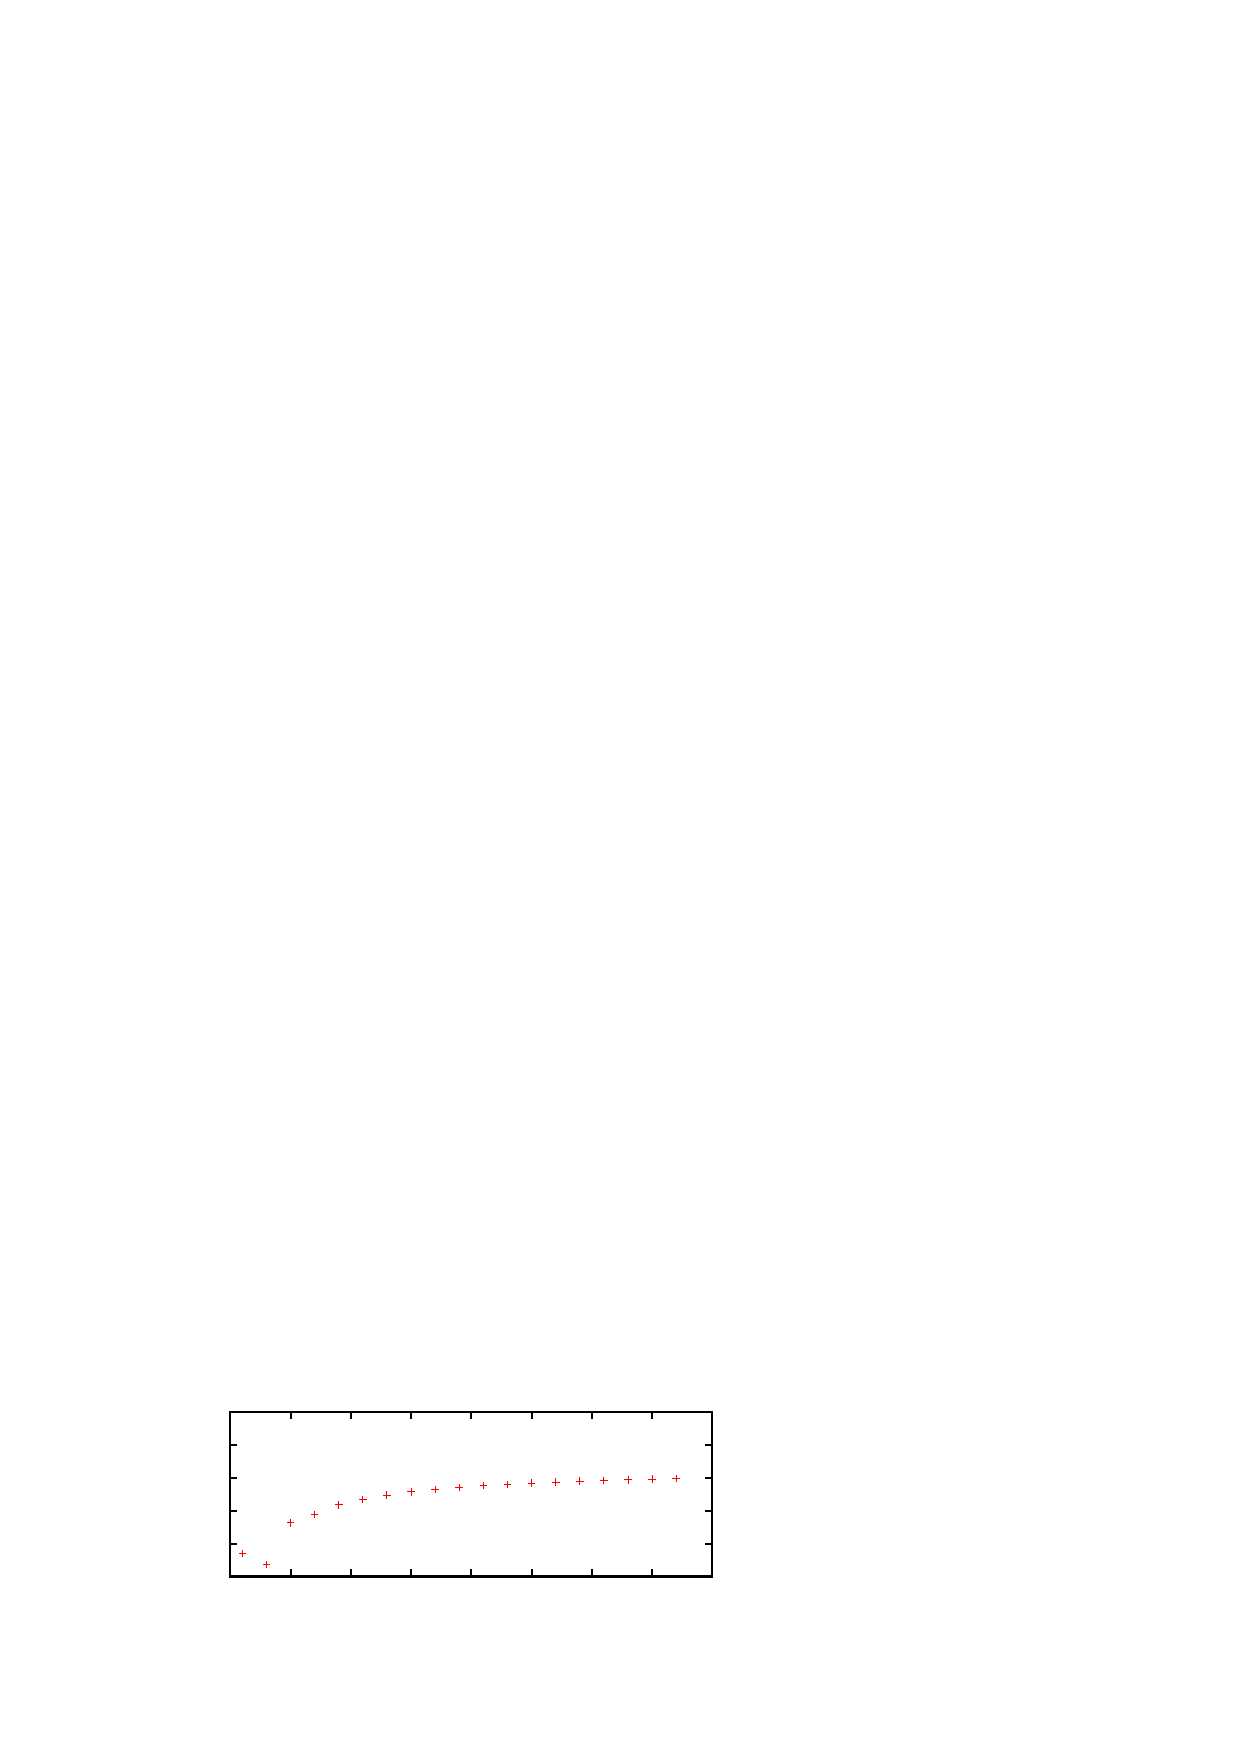
\includegraphics{laurent_f}}%
    \gplfronttext
  \end{picture}%
\endgroup

        %\input{}
        \caption{\em Radius of convergence computed with the 40 first
          coefficients of the Taylor series of the function $A(z)$
          (top) and $F(z)$ (bottom).}
        \label{fig:coeff}        
      \end{center}
    \end{figure}
    The radius of convergence of a series $f(x) = \sum_i f_ix^i$ from
    the general point of view is given by:
    \begin{align}
      R = \frac{1}{\limsup_{i\to\infty}\sqrt[i]{|f_i|}}.
    \end{align}
    Using the numerical values of the coefficients, we find the
    following estimations of the radius of convergence of the series
    for each functions:
    \vspace{18pt}
    {
      \center
      \hfill\makebox{\begin{tabular}{c|c}
        Function $A(z)$ & Function $F(z)$\\
        \hline
        \parbox{3cm}{\vspace{6pt}$\frac{1}{\sqrt[40]{|a_{40}|}}\approx 2.1$} & \parbox{3cm}{\vspace{6pt}$\frac{1}{\sqrt[39]{|f_{39}|}}\approx 2.1$}
      \end{tabular}}\hfill
      \vspace{18pt}
    }

    With a maximal radius of convergence of $\sim 2.1$, this analysis
    seems to predict the first singularity further from the origin
    than what is observed on the numerical simulations.  However, with
    no estimation of the error on these numerical values, no
    conclusion can be drawn to validate or unvalidate the numerical
    solution of the vortex.
  \end{subsection}
\end{section}

\begin{section}{Application to the Monopole in $(3+1)$ dimensions}
  We now turn to the case of the magnetic monopoles. The
  Georgi-Glashow model, which is an $SU(2)$ gauge theory, with a
  potential which allow the Higgs mechanism to take place.  The
  Lagrangian and the ansatz has been presented in section
  \ref{sec:theory_monopole}, and we know derive the Cauchy problem
  which correspond to the analytic continuation of the monopole
  solution.
  
  Again, the first step is to recast the second order system to a
  first order system, introducing two new variables:
  
  \begin{align}
    &M'(r) = S(r),\\
    &S'(r) = 2\frac{M(r)N(r)^2}{r^2}+\lambda v^2\frac{M(r)(M(r)^2-r^2)}{r^2},\\
    &N'(r) = T(r),\\
    &T'(r) = \frac{M(r)(M(r)^2-1)}{r^2}-gv^2\frac{N(r)^2M(r)}{r^2}.
  \end{align}
  Again, we promote $M,N,S$ and $T$ as well as the coordinate $r\to
  z=r+iy$ to the complex field. The Cauchy problem writes:
  \begin{align}
    \partial_y M_I &= S_R,\\
    -\partial_y M_R &= S_I,\\
    \partial_y S_I &= \Re\left[2\frac{(M_R+iM_I)(N_R+iN_I)^2}{z^2}\right.\\
      &\hphantom{= \Re\left[\right.}+\left.\lambda v^2 \frac{(M_R+iM_I)((M_R+iM_I)^2-z^2)}{z^2}\right],\\
      -\partial_y S_R &= \Im\left[2\frac{(M_R+iM_I)(N_R+iN_I)^2}{z^2}\right.\\
        &\hphantom{= \Re\left[\right.}+\left.\lambda v^2 \frac{(M_R+iM_I)((M_R+iM_I)^2-z^2)}{z^2}\right],\\
        \partial_y N_I &= T_R,\\
        -\partial_y N_R &= T_I,\\
        \partial_y T_I &= \Re\left[\frac{(M_R+iM_I)((M_R+iM_I)^2-1)}{z^2}\right.\\
          &\hphantom{=\Re\left[\right.}-\left.gv^2\frac{(N_R+iN_I)^2(M_R+iM_I)}{z^2}\right],\\
          -\partial_y T_R &= \Im\left[\frac{(M_R+iM_I)((M_R+iM_I)^2-1)}{z^2}\right.\\
      &\hphantom{=\Re\left[\right.}-\left.gv^2\frac{(N_R+iN_I)^2(M_R+iM_I)}{z^2}\right],
  \end{align}
  with the following initial conditions:
  \begin{align}
    &M_R(r+i0) = M(r),\\
    &S_R(r+i0) = \frac{\mathrm d}{\mathrm d r}M(r),\\
    &N_R(r+i0) = N(r),\\
    &T_R(r+i0) = \frac{\mathrm d}{\mathrm d r}N(r),\\
    &M_I(r+i0) = 0,\\
    &S_I(r+i0) = 0,\\
    &N_I(r+i0) = 0,\\
    &T_I(r+i0) = 0,\\
  \end{align}
  Approximations of the values of $M$ and $N$ are obtained, as for the
  vortex, by numerical means on a discretization of the interval
  $[0,10]$.
  
  The analytic continuation of the monopole was computed in two
  different case. The first is the BPS limit ($\lambda = 0$), and the
  second with $\lambda = 0.5$. 
  \begin{subsection}{Numerical analytic continuation in the BPS limit}
    This situation is especially useful to check the correctness of
    the implementation of the numerical scheme, as well its
    convergence to the solution. 
    
    Fig. \ref{fig:cm_monopole_f_real_bps}--\ref{fig:cm_monopole_h_imag_bps}
    present real and imaginary parts of functions $M$ and $N$ as a
    result of the numerical integration.

    \begin{figure}[!ht]
      \begin{center}
        % GNUPLOT: LaTeX picture with Postscript
\begingroup
  \makeatletter
  \providecommand\color[2][]{%
    \GenericError{(gnuplot) \space\space\space\@spaces}{%
      Package color not loaded in conjunction with
      terminal option `colourtext'%
    }{See the gnuplot documentation for explanation.%
    }{Either use 'blacktext' in gnuplot or load the package
      color.sty in LaTeX.}%
    \renewcommand\color[2][]{}%
  }%
  \providecommand\includegraphics[2][]{%
    \GenericError{(gnuplot) \space\space\space\@spaces}{%
      Package graphicx or graphics not loaded%
    }{See the gnuplot documentation for explanation.%
    }{The gnuplot epslatex terminal needs graphicx.sty or graphics.sty.}%
    \renewcommand\includegraphics[2][]{}%
  }%
  \providecommand\rotatebox[2]{#2}%
  \@ifundefined{ifGPcolor}{%
    \newif\ifGPcolor
    \GPcolortrue
  }{}%
  \@ifundefined{ifGPblacktext}{%
    \newif\ifGPblacktext
    \GPblacktexttrue
  }{}%
  % define a \g@addto@macro without @ in the name:
  \let\gplgaddtomacro\g@addto@macro
  % define empty templates for all commands taking text:
  \gdef\gplbacktext{}%
  \gdef\gplfronttext{}%
  \makeatother
  \ifGPblacktext
    % no textcolor at all
    \def\colorrgb#1{}%
    \def\colorgray#1{}%
  \else
    % gray or color?
    \ifGPcolor
      \def\colorrgb#1{\color[rgb]{#1}}%
      \def\colorgray#1{\color[gray]{#1}}%
      \expandafter\def\csname LTw\endcsname{\color{white}}%
      \expandafter\def\csname LTb\endcsname{\color{black}}%
      \expandafter\def\csname LTa\endcsname{\color{black}}%
      \expandafter\def\csname LT0\endcsname{\color[rgb]{1,0,0}}%
      \expandafter\def\csname LT1\endcsname{\color[rgb]{0,1,0}}%
      \expandafter\def\csname LT2\endcsname{\color[rgb]{0,0,1}}%
      \expandafter\def\csname LT3\endcsname{\color[rgb]{1,0,1}}%
      \expandafter\def\csname LT4\endcsname{\color[rgb]{0,1,1}}%
      \expandafter\def\csname LT5\endcsname{\color[rgb]{1,1,0}}%
      \expandafter\def\csname LT6\endcsname{\color[rgb]{0,0,0}}%
      \expandafter\def\csname LT7\endcsname{\color[rgb]{1,0.3,0}}%
      \expandafter\def\csname LT8\endcsname{\color[rgb]{0.5,0.5,0.5}}%
    \else
      % gray
      \def\colorrgb#1{\color{black}}%
      \def\colorgray#1{\color[gray]{#1}}%
      \expandafter\def\csname LTw\endcsname{\color{white}}%
      \expandafter\def\csname LTb\endcsname{\color{black}}%
      \expandafter\def\csname LTa\endcsname{\color{black}}%
      \expandafter\def\csname LT0\endcsname{\color{black}}%
      \expandafter\def\csname LT1\endcsname{\color{black}}%
      \expandafter\def\csname LT2\endcsname{\color{black}}%
      \expandafter\def\csname LT3\endcsname{\color{black}}%
      \expandafter\def\csname LT4\endcsname{\color{black}}%
      \expandafter\def\csname LT5\endcsname{\color{black}}%
      \expandafter\def\csname LT6\endcsname{\color{black}}%
      \expandafter\def\csname LT7\endcsname{\color{black}}%
      \expandafter\def\csname LT8\endcsname{\color{black}}%
    \fi
  \fi
  \setlength{\unitlength}{0.0500bp}%
  \begin{picture}(6236.00,2834.00)%
    \gplgaddtomacro\gplbacktext{%
    }%
    \gplgaddtomacro\gplfronttext{%
      \csname LTb\endcsname%
      \put(1046,517){\makebox(0,0){\strut{}-10}}%
      \put(2082,517){\makebox(0,0){\strut{}-5}}%
      \put(3118,517){\makebox(0,0){\strut{} 0}}%
      \put(4154,517){\makebox(0,0){\strut{} 5}}%
      \put(5190,517){\makebox(0,0){\strut{} 10}}%
      \put(3118,187){\makebox(0,0){\strut{}$x$}}%
      \put(874,803){\makebox(0,0)[r]{\strut{} 0}}%
      \put(874,1093){\makebox(0,0)[r]{\strut{} 2}}%
      \put(874,1383){\makebox(0,0)[r]{\strut{} 4}}%
      \put(874,1671){\makebox(0,0)[r]{\strut{} 6}}%
      \put(874,1961){\makebox(0,0)[r]{\strut{} 8}}%
      \put(874,2251){\makebox(0,0)[r]{\strut{} 10}}%
      \put(412,1527){\rotatebox{-270}{\makebox(0,0){\strut{}$y$}}}%
      \put(5633,809){\makebox(0,0)[l]{\strut{}-10}}%
      \put(5633,1167){\makebox(0,0)[l]{\strut{}-5}}%
      \put(5633,1526){\makebox(0,0)[l]{\strut{} 0}}%
      \put(5633,1885){\makebox(0,0)[l]{\strut{} 5}}%
      \put(5633,2243){\makebox(0,0)[l]{\strut{} 10}}%
    }%
    \gplbacktext
    \put(0,0){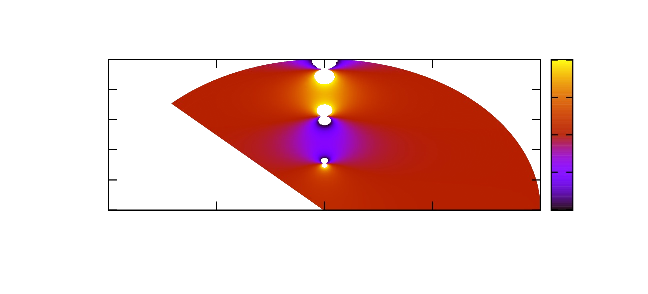
\includegraphics{monopole_anal_f_real_bps}}%
    \gplfronttext
  \end{picture}%
\endgroup

        \caption{\em Real part of the function $N(z)$ in the BPS
          limit. All the singularities lie on the imaginary axis. The
          function is even under conjugation: $\Re N(z) = \Re N(\bar
          z)$.}
        \label{fig:cm_monopole_f_real_bps}
      \end{center}
    \end{figure}

    \begin{figure}[!ht]
      \begin{center}
        % GNUPLOT: LaTeX picture with Postscript
\begingroup
  \makeatletter
  \providecommand\color[2][]{%
    \GenericError{(gnuplot) \space\space\space\@spaces}{%
      Package color not loaded in conjunction with
      terminal option `colourtext'%
    }{See the gnuplot documentation for explanation.%
    }{Either use 'blacktext' in gnuplot or load the package
      color.sty in LaTeX.}%
    \renewcommand\color[2][]{}%
  }%
  \providecommand\includegraphics[2][]{%
    \GenericError{(gnuplot) \space\space\space\@spaces}{%
      Package graphicx or graphics not loaded%
    }{See the gnuplot documentation for explanation.%
    }{The gnuplot epslatex terminal needs graphicx.sty or graphics.sty.}%
    \renewcommand\includegraphics[2][]{}%
  }%
  \providecommand\rotatebox[2]{#2}%
  \@ifundefined{ifGPcolor}{%
    \newif\ifGPcolor
    \GPcolortrue
  }{}%
  \@ifundefined{ifGPblacktext}{%
    \newif\ifGPblacktext
    \GPblacktexttrue
  }{}%
  % define a \g@addto@macro without @ in the name:
  \let\gplgaddtomacro\g@addto@macro
  % define empty templates for all commands taking text:
  \gdef\gplbacktext{}%
  \gdef\gplfronttext{}%
  \makeatother
  \ifGPblacktext
    % no textcolor at all
    \def\colorrgb#1{}%
    \def\colorgray#1{}%
  \else
    % gray or color?
    \ifGPcolor
      \def\colorrgb#1{\color[rgb]{#1}}%
      \def\colorgray#1{\color[gray]{#1}}%
      \expandafter\def\csname LTw\endcsname{\color{white}}%
      \expandafter\def\csname LTb\endcsname{\color{black}}%
      \expandafter\def\csname LTa\endcsname{\color{black}}%
      \expandafter\def\csname LT0\endcsname{\color[rgb]{1,0,0}}%
      \expandafter\def\csname LT1\endcsname{\color[rgb]{0,1,0}}%
      \expandafter\def\csname LT2\endcsname{\color[rgb]{0,0,1}}%
      \expandafter\def\csname LT3\endcsname{\color[rgb]{1,0,1}}%
      \expandafter\def\csname LT4\endcsname{\color[rgb]{0,1,1}}%
      \expandafter\def\csname LT5\endcsname{\color[rgb]{1,1,0}}%
      \expandafter\def\csname LT6\endcsname{\color[rgb]{0,0,0}}%
      \expandafter\def\csname LT7\endcsname{\color[rgb]{1,0.3,0}}%
      \expandafter\def\csname LT8\endcsname{\color[rgb]{0.5,0.5,0.5}}%
    \else
      % gray
      \def\colorrgb#1{\color{black}}%
      \def\colorgray#1{\color[gray]{#1}}%
      \expandafter\def\csname LTw\endcsname{\color{white}}%
      \expandafter\def\csname LTb\endcsname{\color{black}}%
      \expandafter\def\csname LTa\endcsname{\color{black}}%
      \expandafter\def\csname LT0\endcsname{\color{black}}%
      \expandafter\def\csname LT1\endcsname{\color{black}}%
      \expandafter\def\csname LT2\endcsname{\color{black}}%
      \expandafter\def\csname LT3\endcsname{\color{black}}%
      \expandafter\def\csname LT4\endcsname{\color{black}}%
      \expandafter\def\csname LT5\endcsname{\color{black}}%
      \expandafter\def\csname LT6\endcsname{\color{black}}%
      \expandafter\def\csname LT7\endcsname{\color{black}}%
      \expandafter\def\csname LT8\endcsname{\color{black}}%
    \fi
  \fi
  \setlength{\unitlength}{0.0500bp}%
  \begin{picture}(6236.00,2834.00)%
    \gplgaddtomacro\gplbacktext{%
    }%
    \gplgaddtomacro\gplfronttext{%
      \csname LTb\endcsname%
      \put(1046,517){\makebox(0,0){\strut{}-10}}%
      \put(2082,517){\makebox(0,0){\strut{}-5}}%
      \put(3118,517){\makebox(0,0){\strut{} 0}}%
      \put(4154,517){\makebox(0,0){\strut{} 5}}%
      \put(5190,517){\makebox(0,0){\strut{} 10}}%
      \put(3118,187){\makebox(0,0){\strut{}$x$}}%
      \put(874,803){\makebox(0,0)[r]{\strut{} 0}}%
      \put(874,1093){\makebox(0,0)[r]{\strut{} 2}}%
      \put(874,1383){\makebox(0,0)[r]{\strut{} 4}}%
      \put(874,1671){\makebox(0,0)[r]{\strut{} 6}}%
      \put(874,1961){\makebox(0,0)[r]{\strut{} 8}}%
      \put(874,2251){\makebox(0,0)[r]{\strut{} 10}}%
      \put(412,1527){\rotatebox{-270}{\makebox(0,0){\strut{}$y$}}}%
      \put(5633,809){\makebox(0,0)[l]{\strut{}-10}}%
      \put(5633,1167){\makebox(0,0)[l]{\strut{}-5}}%
      \put(5633,1526){\makebox(0,0)[l]{\strut{} 0}}%
      \put(5633,1885){\makebox(0,0)[l]{\strut{} 5}}%
      \put(5633,2243){\makebox(0,0)[l]{\strut{} 10}}%
    }%
    \gplbacktext
    \put(0,0){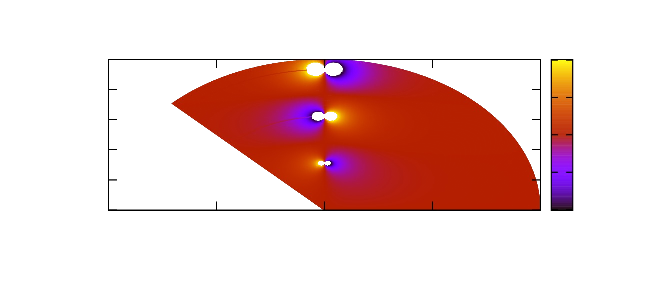
\includegraphics{monopole_anal_f_imag_bps}}%
    \gplfronttext
  \end{picture}%
\endgroup

        \caption{\em Imaginary part of the function $N(z)$ in the BPS
          limit. The function is odd under conjugation: $\Im N(z) =
          -\Im N(\bar z)$.}
        \label{fig:cm_monopole_f_imag_bps}
      \end{center}
    \end{figure}

    \begin{figure}[!ht]
      \begin{center}
        % GNUPLOT: LaTeX picture with Postscript
\begingroup
  \makeatletter
  \providecommand\color[2][]{%
    \GenericError{(gnuplot) \space\space\space\@spaces}{%
      Package color not loaded in conjunction with
      terminal option `colourtext'%
    }{See the gnuplot documentation for explanation.%
    }{Either use 'blacktext' in gnuplot or load the package
      color.sty in LaTeX.}%
    \renewcommand\color[2][]{}%
  }%
  \providecommand\includegraphics[2][]{%
    \GenericError{(gnuplot) \space\space\space\@spaces}{%
      Package graphicx or graphics not loaded%
    }{See the gnuplot documentation for explanation.%
    }{The gnuplot epslatex terminal needs graphicx.sty or graphics.sty.}%
    \renewcommand\includegraphics[2][]{}%
  }%
  \providecommand\rotatebox[2]{#2}%
  \@ifundefined{ifGPcolor}{%
    \newif\ifGPcolor
    \GPcolortrue
  }{}%
  \@ifundefined{ifGPblacktext}{%
    \newif\ifGPblacktext
    \GPblacktexttrue
  }{}%
  % define a \g@addto@macro without @ in the name:
  \let\gplgaddtomacro\g@addto@macro
  % define empty templates for all commands taking text:
  \gdef\gplbacktext{}%
  \gdef\gplfronttext{}%
  \makeatother
  \ifGPblacktext
    % no textcolor at all
    \def\colorrgb#1{}%
    \def\colorgray#1{}%
  \else
    % gray or color?
    \ifGPcolor
      \def\colorrgb#1{\color[rgb]{#1}}%
      \def\colorgray#1{\color[gray]{#1}}%
      \expandafter\def\csname LTw\endcsname{\color{white}}%
      \expandafter\def\csname LTb\endcsname{\color{black}}%
      \expandafter\def\csname LTa\endcsname{\color{black}}%
      \expandafter\def\csname LT0\endcsname{\color[rgb]{1,0,0}}%
      \expandafter\def\csname LT1\endcsname{\color[rgb]{0,1,0}}%
      \expandafter\def\csname LT2\endcsname{\color[rgb]{0,0,1}}%
      \expandafter\def\csname LT3\endcsname{\color[rgb]{1,0,1}}%
      \expandafter\def\csname LT4\endcsname{\color[rgb]{0,1,1}}%
      \expandafter\def\csname LT5\endcsname{\color[rgb]{1,1,0}}%
      \expandafter\def\csname LT6\endcsname{\color[rgb]{0,0,0}}%
      \expandafter\def\csname LT7\endcsname{\color[rgb]{1,0.3,0}}%
      \expandafter\def\csname LT8\endcsname{\color[rgb]{0.5,0.5,0.5}}%
    \else
      % gray
      \def\colorrgb#1{\color{black}}%
      \def\colorgray#1{\color[gray]{#1}}%
      \expandafter\def\csname LTw\endcsname{\color{white}}%
      \expandafter\def\csname LTb\endcsname{\color{black}}%
      \expandafter\def\csname LTa\endcsname{\color{black}}%
      \expandafter\def\csname LT0\endcsname{\color{black}}%
      \expandafter\def\csname LT1\endcsname{\color{black}}%
      \expandafter\def\csname LT2\endcsname{\color{black}}%
      \expandafter\def\csname LT3\endcsname{\color{black}}%
      \expandafter\def\csname LT4\endcsname{\color{black}}%
      \expandafter\def\csname LT5\endcsname{\color{black}}%
      \expandafter\def\csname LT6\endcsname{\color{black}}%
      \expandafter\def\csname LT7\endcsname{\color{black}}%
      \expandafter\def\csname LT8\endcsname{\color{black}}%
    \fi
  \fi
  \setlength{\unitlength}{0.0500bp}%
  \begin{picture}(6236.00,2834.00)%
    \gplgaddtomacro\gplbacktext{%
    }%
    \gplgaddtomacro\gplfronttext{%
      \csname LTb\endcsname%
      \put(1046,517){\makebox(0,0){\strut{}-10}}%
      \put(2082,517){\makebox(0,0){\strut{}-5}}%
      \put(3118,517){\makebox(0,0){\strut{} 0}}%
      \put(4154,517){\makebox(0,0){\strut{} 5}}%
      \put(5190,517){\makebox(0,0){\strut{} 10}}%
      \put(3118,187){\makebox(0,0){\strut{}$x$}}%
      \put(874,803){\makebox(0,0)[r]{\strut{} 0}}%
      \put(874,1093){\makebox(0,0)[r]{\strut{} 2}}%
      \put(874,1383){\makebox(0,0)[r]{\strut{} 4}}%
      \put(874,1671){\makebox(0,0)[r]{\strut{} 6}}%
      \put(874,1961){\makebox(0,0)[r]{\strut{} 8}}%
      \put(874,2251){\makebox(0,0)[r]{\strut{} 10}}%
      \put(412,1527){\rotatebox{-270}{\makebox(0,0){\strut{}$y$}}}%
      \put(5633,811){\makebox(0,0)[l]{\strut{}-5}}%
      \put(5633,1288){\makebox(0,0)[l]{\strut{} 0}}%
      \put(5633,1764){\makebox(0,0)[l]{\strut{} 5}}%
      \put(5633,2241){\makebox(0,0)[l]{\strut{} 10}}%
    }%
    \gplbacktext
    \put(0,0){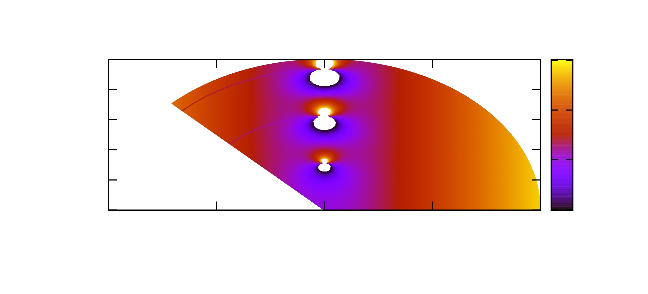
\includegraphics{monopole_anal_h_real_bps}}%
    \gplfronttext
  \end{picture}%
\endgroup

        \caption{\em Real part of the function $M(z)$ (not $M(z)/z$,
          as on Fig. \ref{fig:2d_monopole_f}) in the BPS
          limit. All the singularities lie on the imaginary axis. The
          function is even under conjugation: $\Re N(z) = \Re N(\bar
          z)$.}
        \label{fig:cm_monopole_h_real_bps}
      \end{center}
    \end{figure}

    \begin{figure}[!ht]
      \begin{center}
        % GNUPLOT: LaTeX picture with Postscript
\begingroup
  \makeatletter
  \providecommand\color[2][]{%
    \GenericError{(gnuplot) \space\space\space\@spaces}{%
      Package color not loaded in conjunction with
      terminal option `colourtext'%
    }{See the gnuplot documentation for explanation.%
    }{Either use 'blacktext' in gnuplot or load the package
      color.sty in LaTeX.}%
    \renewcommand\color[2][]{}%
  }%
  \providecommand\includegraphics[2][]{%
    \GenericError{(gnuplot) \space\space\space\@spaces}{%
      Package graphicx or graphics not loaded%
    }{See the gnuplot documentation for explanation.%
    }{The gnuplot epslatex terminal needs graphicx.sty or graphics.sty.}%
    \renewcommand\includegraphics[2][]{}%
  }%
  \providecommand\rotatebox[2]{#2}%
  \@ifundefined{ifGPcolor}{%
    \newif\ifGPcolor
    \GPcolortrue
  }{}%
  \@ifundefined{ifGPblacktext}{%
    \newif\ifGPblacktext
    \GPblacktexttrue
  }{}%
  % define a \g@addto@macro without @ in the name:
  \let\gplgaddtomacro\g@addto@macro
  % define empty templates for all commands taking text:
  \gdef\gplbacktext{}%
  \gdef\gplfronttext{}%
  \makeatother
  \ifGPblacktext
    % no textcolor at all
    \def\colorrgb#1{}%
    \def\colorgray#1{}%
  \else
    % gray or color?
    \ifGPcolor
      \def\colorrgb#1{\color[rgb]{#1}}%
      \def\colorgray#1{\color[gray]{#1}}%
      \expandafter\def\csname LTw\endcsname{\color{white}}%
      \expandafter\def\csname LTb\endcsname{\color{black}}%
      \expandafter\def\csname LTa\endcsname{\color{black}}%
      \expandafter\def\csname LT0\endcsname{\color[rgb]{1,0,0}}%
      \expandafter\def\csname LT1\endcsname{\color[rgb]{0,1,0}}%
      \expandafter\def\csname LT2\endcsname{\color[rgb]{0,0,1}}%
      \expandafter\def\csname LT3\endcsname{\color[rgb]{1,0,1}}%
      \expandafter\def\csname LT4\endcsname{\color[rgb]{0,1,1}}%
      \expandafter\def\csname LT5\endcsname{\color[rgb]{1,1,0}}%
      \expandafter\def\csname LT6\endcsname{\color[rgb]{0,0,0}}%
      \expandafter\def\csname LT7\endcsname{\color[rgb]{1,0.3,0}}%
      \expandafter\def\csname LT8\endcsname{\color[rgb]{0.5,0.5,0.5}}%
    \else
      % gray
      \def\colorrgb#1{\color{black}}%
      \def\colorgray#1{\color[gray]{#1}}%
      \expandafter\def\csname LTw\endcsname{\color{white}}%
      \expandafter\def\csname LTb\endcsname{\color{black}}%
      \expandafter\def\csname LTa\endcsname{\color{black}}%
      \expandafter\def\csname LT0\endcsname{\color{black}}%
      \expandafter\def\csname LT1\endcsname{\color{black}}%
      \expandafter\def\csname LT2\endcsname{\color{black}}%
      \expandafter\def\csname LT3\endcsname{\color{black}}%
      \expandafter\def\csname LT4\endcsname{\color{black}}%
      \expandafter\def\csname LT5\endcsname{\color{black}}%
      \expandafter\def\csname LT6\endcsname{\color{black}}%
      \expandafter\def\csname LT7\endcsname{\color{black}}%
      \expandafter\def\csname LT8\endcsname{\color{black}}%
    \fi
  \fi
  \setlength{\unitlength}{0.0500bp}%
  \begin{picture}(6236.00,2834.00)%
    \gplgaddtomacro\gplbacktext{%
    }%
    \gplgaddtomacro\gplfronttext{%
      \csname LTb\endcsname%
      \put(1046,517){\makebox(0,0){\strut{}-10}}%
      \put(2082,517){\makebox(0,0){\strut{}-5}}%
      \put(3118,517){\makebox(0,0){\strut{} 0}}%
      \put(4154,517){\makebox(0,0){\strut{} 5}}%
      \put(5190,517){\makebox(0,0){\strut{} 10}}%
      \put(3118,187){\makebox(0,0){\strut{}$x$}}%
      \put(874,803){\makebox(0,0)[r]{\strut{} 0}}%
      \put(874,1093){\makebox(0,0)[r]{\strut{} 2}}%
      \put(874,1383){\makebox(0,0)[r]{\strut{} 4}}%
      \put(874,1671){\makebox(0,0)[r]{\strut{} 6}}%
      \put(874,1961){\makebox(0,0)[r]{\strut{} 8}}%
      \put(874,2251){\makebox(0,0)[r]{\strut{} 10}}%
      \put(412,1527){\rotatebox{-270}{\makebox(0,0){\strut{}$y$}}}%
      \put(5633,811){\makebox(0,0)[l]{\strut{}-5}}%
      \put(5633,1288){\makebox(0,0)[l]{\strut{} 0}}%
      \put(5633,1764){\makebox(0,0)[l]{\strut{} 5}}%
      \put(5633,2241){\makebox(0,0)[l]{\strut{} 10}}%
    }%
    \gplbacktext
    \put(0,0){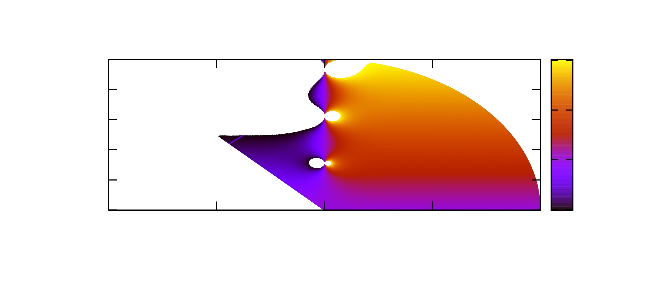
\includegraphics{monopole_anal_h_imag_bps}}%
    \gplfronttext
  \end{picture}%
\endgroup

        \caption{\em Imaginary part of the function $N(z)$ in the BPS
          limit. The function is odd under conjugation: $\Im N(z) =
          -\Im N(\bar z)$. The extended white regions correspond to
          out of range values.}
        \label{fig:cm_monopole_h_imag_bps}
      \end{center}
    \end{figure}
    Beside the fact that the numerical scheme has shown to converge
    to the solution, the most important feature to notice is that
    all the singularities lie on the imaginary axis.
    
    The next subsection show the behaviour of the solution when the
    Higgs coupling constant $\lambda$ is slightly increased.
  \end{subsection}
  \begin{subsection}{Numerical analytic continuation, $\lambda \neq 0$}
    In the BPS limit, all the singularities of the functions were lying on
    the imaginary axis, but it is not the case anymore, as can be seen
    on Fig. \ref{fig:cm_monopole_f_real}--\ref{fig:cm_monopole_h_imag}.

    Only the one which is closest to the origin stays on the imaginary
    axis, and all the other have been shifted to the negative real
    half complex plane.
    \begin{figure}[!ht]
      \begin{center}
        % GNUPLOT: LaTeX picture with Postscript
\begingroup
  \makeatletter
  \providecommand\color[2][]{%
    \GenericError{(gnuplot) \space\space\space\@spaces}{%
      Package color not loaded in conjunction with
      terminal option `colourtext'%
    }{See the gnuplot documentation for explanation.%
    }{Either use 'blacktext' in gnuplot or load the package
      color.sty in LaTeX.}%
    \renewcommand\color[2][]{}%
  }%
  \providecommand\includegraphics[2][]{%
    \GenericError{(gnuplot) \space\space\space\@spaces}{%
      Package graphicx or graphics not loaded%
    }{See the gnuplot documentation for explanation.%
    }{The gnuplot epslatex terminal needs graphicx.sty or graphics.sty.}%
    \renewcommand\includegraphics[2][]{}%
  }%
  \providecommand\rotatebox[2]{#2}%
  \@ifundefined{ifGPcolor}{%
    \newif\ifGPcolor
    \GPcolortrue
  }{}%
  \@ifundefined{ifGPblacktext}{%
    \newif\ifGPblacktext
    \GPblacktexttrue
  }{}%
  % define a \g@addto@macro without @ in the name:
  \let\gplgaddtomacro\g@addto@macro
  % define empty templates for all commands taking text:
  \gdef\gplbacktext{}%
  \gdef\gplfronttext{}%
  \makeatother
  \ifGPblacktext
    % no textcolor at all
    \def\colorrgb#1{}%
    \def\colorgray#1{}%
  \else
    % gray or color?
    \ifGPcolor
      \def\colorrgb#1{\color[rgb]{#1}}%
      \def\colorgray#1{\color[gray]{#1}}%
      \expandafter\def\csname LTw\endcsname{\color{white}}%
      \expandafter\def\csname LTb\endcsname{\color{black}}%
      \expandafter\def\csname LTa\endcsname{\color{black}}%
      \expandafter\def\csname LT0\endcsname{\color[rgb]{1,0,0}}%
      \expandafter\def\csname LT1\endcsname{\color[rgb]{0,1,0}}%
      \expandafter\def\csname LT2\endcsname{\color[rgb]{0,0,1}}%
      \expandafter\def\csname LT3\endcsname{\color[rgb]{1,0,1}}%
      \expandafter\def\csname LT4\endcsname{\color[rgb]{0,1,1}}%
      \expandafter\def\csname LT5\endcsname{\color[rgb]{1,1,0}}%
      \expandafter\def\csname LT6\endcsname{\color[rgb]{0,0,0}}%
      \expandafter\def\csname LT7\endcsname{\color[rgb]{1,0.3,0}}%
      \expandafter\def\csname LT8\endcsname{\color[rgb]{0.5,0.5,0.5}}%
    \else
      % gray
      \def\colorrgb#1{\color{black}}%
      \def\colorgray#1{\color[gray]{#1}}%
      \expandafter\def\csname LTw\endcsname{\color{white}}%
      \expandafter\def\csname LTb\endcsname{\color{black}}%
      \expandafter\def\csname LTa\endcsname{\color{black}}%
      \expandafter\def\csname LT0\endcsname{\color{black}}%
      \expandafter\def\csname LT1\endcsname{\color{black}}%
      \expandafter\def\csname LT2\endcsname{\color{black}}%
      \expandafter\def\csname LT3\endcsname{\color{black}}%
      \expandafter\def\csname LT4\endcsname{\color{black}}%
      \expandafter\def\csname LT5\endcsname{\color{black}}%
      \expandafter\def\csname LT6\endcsname{\color{black}}%
      \expandafter\def\csname LT7\endcsname{\color{black}}%
      \expandafter\def\csname LT8\endcsname{\color{black}}%
    \fi
  \fi
  \setlength{\unitlength}{0.0500bp}%
  \begin{picture}(6236.00,2834.00)%
    \gplgaddtomacro\gplbacktext{%
    }%
    \gplgaddtomacro\gplfronttext{%
      \csname LTb\endcsname%
      \put(1046,517){\makebox(0,0){\strut{}-10}}%
      \put(2082,517){\makebox(0,0){\strut{}-5}}%
      \put(3118,517){\makebox(0,0){\strut{} 0}}%
      \put(4154,517){\makebox(0,0){\strut{} 5}}%
      \put(5190,517){\makebox(0,0){\strut{} 10}}%
      \put(3118,187){\makebox(0,0){\strut{}$x$}}%
      \put(874,803){\makebox(0,0)[r]{\strut{} 0}}%
      \put(874,1093){\makebox(0,0)[r]{\strut{} 2}}%
      \put(874,1383){\makebox(0,0)[r]{\strut{} 4}}%
      \put(874,1671){\makebox(0,0)[r]{\strut{} 6}}%
      \put(874,1961){\makebox(0,0)[r]{\strut{} 8}}%
      \put(874,2251){\makebox(0,0)[r]{\strut{} 10}}%
      \put(412,1527){\rotatebox{-270}{\makebox(0,0){\strut{}$y$}}}%
      \put(5633,809){\makebox(0,0)[l]{\strut{}-10}}%
      \put(5633,1167){\makebox(0,0)[l]{\strut{}-5}}%
      \put(5633,1526){\makebox(0,0)[l]{\strut{} 0}}%
      \put(5633,1885){\makebox(0,0)[l]{\strut{} 5}}%
      \put(5633,2243){\makebox(0,0)[l]{\strut{} 10}}%
    }%
    \gplbacktext
    \put(0,0){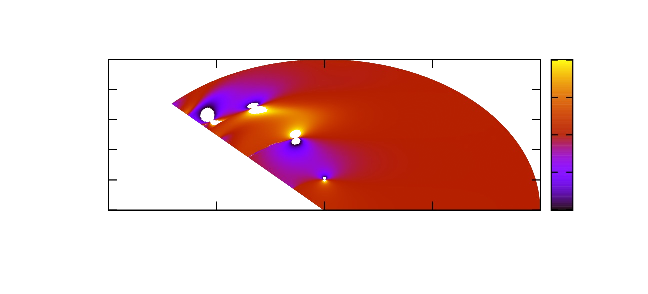
\includegraphics{monopole_anal_f_real}}%
    \gplfronttext
  \end{picture}%
\endgroup

        \caption{\em Real part of the function $N(z)$ with $\lambda =
          0.5$. The singularity which is closest to the origin lie on
          the imaginary axis ($z_0\approx 0+2.05i$). In comparison to
          the BPS limit, all the other singularities are now shifted
          to the negative imaginary half plane (coordinates of the
          second one: $z_0\approx -1.32+4.8i$). The function is even
          under conjugation: $\Re N(z) = \Re N(\bar z)$.}
        \label{fig:cm_monopole_f_real}
      \end{center}
    \end{figure}

    \begin{figure}[!ht]
      \begin{center}
        % GNUPLOT: LaTeX picture with Postscript
\begingroup
  \makeatletter
  \providecommand\color[2][]{%
    \GenericError{(gnuplot) \space\space\space\@spaces}{%
      Package color not loaded in conjunction with
      terminal option `colourtext'%
    }{See the gnuplot documentation for explanation.%
    }{Either use 'blacktext' in gnuplot or load the package
      color.sty in LaTeX.}%
    \renewcommand\color[2][]{}%
  }%
  \providecommand\includegraphics[2][]{%
    \GenericError{(gnuplot) \space\space\space\@spaces}{%
      Package graphicx or graphics not loaded%
    }{See the gnuplot documentation for explanation.%
    }{The gnuplot epslatex terminal needs graphicx.sty or graphics.sty.}%
    \renewcommand\includegraphics[2][]{}%
  }%
  \providecommand\rotatebox[2]{#2}%
  \@ifundefined{ifGPcolor}{%
    \newif\ifGPcolor
    \GPcolortrue
  }{}%
  \@ifundefined{ifGPblacktext}{%
    \newif\ifGPblacktext
    \GPblacktexttrue
  }{}%
  % define a \g@addto@macro without @ in the name:
  \let\gplgaddtomacro\g@addto@macro
  % define empty templates for all commands taking text:
  \gdef\gplbacktext{}%
  \gdef\gplfronttext{}%
  \makeatother
  \ifGPblacktext
    % no textcolor at all
    \def\colorrgb#1{}%
    \def\colorgray#1{}%
  \else
    % gray or color?
    \ifGPcolor
      \def\colorrgb#1{\color[rgb]{#1}}%
      \def\colorgray#1{\color[gray]{#1}}%
      \expandafter\def\csname LTw\endcsname{\color{white}}%
      \expandafter\def\csname LTb\endcsname{\color{black}}%
      \expandafter\def\csname LTa\endcsname{\color{black}}%
      \expandafter\def\csname LT0\endcsname{\color[rgb]{1,0,0}}%
      \expandafter\def\csname LT1\endcsname{\color[rgb]{0,1,0}}%
      \expandafter\def\csname LT2\endcsname{\color[rgb]{0,0,1}}%
      \expandafter\def\csname LT3\endcsname{\color[rgb]{1,0,1}}%
      \expandafter\def\csname LT4\endcsname{\color[rgb]{0,1,1}}%
      \expandafter\def\csname LT5\endcsname{\color[rgb]{1,1,0}}%
      \expandafter\def\csname LT6\endcsname{\color[rgb]{0,0,0}}%
      \expandafter\def\csname LT7\endcsname{\color[rgb]{1,0.3,0}}%
      \expandafter\def\csname LT8\endcsname{\color[rgb]{0.5,0.5,0.5}}%
    \else
      % gray
      \def\colorrgb#1{\color{black}}%
      \def\colorgray#1{\color[gray]{#1}}%
      \expandafter\def\csname LTw\endcsname{\color{white}}%
      \expandafter\def\csname LTb\endcsname{\color{black}}%
      \expandafter\def\csname LTa\endcsname{\color{black}}%
      \expandafter\def\csname LT0\endcsname{\color{black}}%
      \expandafter\def\csname LT1\endcsname{\color{black}}%
      \expandafter\def\csname LT2\endcsname{\color{black}}%
      \expandafter\def\csname LT3\endcsname{\color{black}}%
      \expandafter\def\csname LT4\endcsname{\color{black}}%
      \expandafter\def\csname LT5\endcsname{\color{black}}%
      \expandafter\def\csname LT6\endcsname{\color{black}}%
      \expandafter\def\csname LT7\endcsname{\color{black}}%
      \expandafter\def\csname LT8\endcsname{\color{black}}%
    \fi
  \fi
  \setlength{\unitlength}{0.0500bp}%
  \begin{picture}(6236.00,2834.00)%
    \gplgaddtomacro\gplbacktext{%
    }%
    \gplgaddtomacro\gplfronttext{%
      \csname LTb\endcsname%
      \put(1046,517){\makebox(0,0){\strut{}-10}}%
      \put(2082,517){\makebox(0,0){\strut{}-5}}%
      \put(3118,517){\makebox(0,0){\strut{} 0}}%
      \put(4154,517){\makebox(0,0){\strut{} 5}}%
      \put(5190,517){\makebox(0,0){\strut{} 10}}%
      \put(3118,187){\makebox(0,0){\strut{}$x$}}%
      \put(874,803){\makebox(0,0)[r]{\strut{} 0}}%
      \put(874,1093){\makebox(0,0)[r]{\strut{} 2}}%
      \put(874,1383){\makebox(0,0)[r]{\strut{} 4}}%
      \put(874,1671){\makebox(0,0)[r]{\strut{} 6}}%
      \put(874,1961){\makebox(0,0)[r]{\strut{} 8}}%
      \put(874,2251){\makebox(0,0)[r]{\strut{} 10}}%
      \put(412,1527){\rotatebox{-270}{\makebox(0,0){\strut{}$y$}}}%
      \put(5633,809){\makebox(0,0)[l]{\strut{}-10}}%
      \put(5633,1167){\makebox(0,0)[l]{\strut{}-5}}%
      \put(5633,1526){\makebox(0,0)[l]{\strut{} 0}}%
      \put(5633,1885){\makebox(0,0)[l]{\strut{} 5}}%
      \put(5633,2243){\makebox(0,0)[l]{\strut{} 10}}%
    }%
    \gplbacktext
    \put(0,0){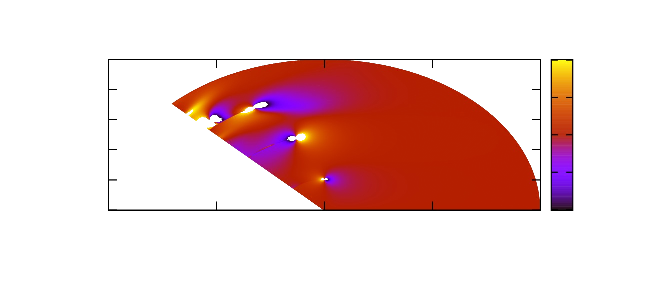
\includegraphics{monopole_anal_f_imag}}%
    \gplfronttext
  \end{picture}%
\endgroup

        \caption{\em Imaginary part of the function $N(z)$ with
          $\lambda = 0.5$. The function is odd under conjugation: $\Im
          N(z) = -\Im N(\bar z)$.}
        \label{fig:cm_monopole_f_imag}
      \end{center}
    \end{figure}

    \begin{figure}[!ht]
      \begin{center}
        % GNUPLOT: LaTeX picture with Postscript
\begingroup
  \makeatletter
  \providecommand\color[2][]{%
    \GenericError{(gnuplot) \space\space\space\@spaces}{%
      Package color not loaded in conjunction with
      terminal option `colourtext'%
    }{See the gnuplot documentation for explanation.%
    }{Either use 'blacktext' in gnuplot or load the package
      color.sty in LaTeX.}%
    \renewcommand\color[2][]{}%
  }%
  \providecommand\includegraphics[2][]{%
    \GenericError{(gnuplot) \space\space\space\@spaces}{%
      Package graphicx or graphics not loaded%
    }{See the gnuplot documentation for explanation.%
    }{The gnuplot epslatex terminal needs graphicx.sty or graphics.sty.}%
    \renewcommand\includegraphics[2][]{}%
  }%
  \providecommand\rotatebox[2]{#2}%
  \@ifundefined{ifGPcolor}{%
    \newif\ifGPcolor
    \GPcolortrue
  }{}%
  \@ifundefined{ifGPblacktext}{%
    \newif\ifGPblacktext
    \GPblacktexttrue
  }{}%
  % define a \g@addto@macro without @ in the name:
  \let\gplgaddtomacro\g@addto@macro
  % define empty templates for all commands taking text:
  \gdef\gplbacktext{}%
  \gdef\gplfronttext{}%
  \makeatother
  \ifGPblacktext
    % no textcolor at all
    \def\colorrgb#1{}%
    \def\colorgray#1{}%
  \else
    % gray or color?
    \ifGPcolor
      \def\colorrgb#1{\color[rgb]{#1}}%
      \def\colorgray#1{\color[gray]{#1}}%
      \expandafter\def\csname LTw\endcsname{\color{white}}%
      \expandafter\def\csname LTb\endcsname{\color{black}}%
      \expandafter\def\csname LTa\endcsname{\color{black}}%
      \expandafter\def\csname LT0\endcsname{\color[rgb]{1,0,0}}%
      \expandafter\def\csname LT1\endcsname{\color[rgb]{0,1,0}}%
      \expandafter\def\csname LT2\endcsname{\color[rgb]{0,0,1}}%
      \expandafter\def\csname LT3\endcsname{\color[rgb]{1,0,1}}%
      \expandafter\def\csname LT4\endcsname{\color[rgb]{0,1,1}}%
      \expandafter\def\csname LT5\endcsname{\color[rgb]{1,1,0}}%
      \expandafter\def\csname LT6\endcsname{\color[rgb]{0,0,0}}%
      \expandafter\def\csname LT7\endcsname{\color[rgb]{1,0.3,0}}%
      \expandafter\def\csname LT8\endcsname{\color[rgb]{0.5,0.5,0.5}}%
    \else
      % gray
      \def\colorrgb#1{\color{black}}%
      \def\colorgray#1{\color[gray]{#1}}%
      \expandafter\def\csname LTw\endcsname{\color{white}}%
      \expandafter\def\csname LTb\endcsname{\color{black}}%
      \expandafter\def\csname LTa\endcsname{\color{black}}%
      \expandafter\def\csname LT0\endcsname{\color{black}}%
      \expandafter\def\csname LT1\endcsname{\color{black}}%
      \expandafter\def\csname LT2\endcsname{\color{black}}%
      \expandafter\def\csname LT3\endcsname{\color{black}}%
      \expandafter\def\csname LT4\endcsname{\color{black}}%
      \expandafter\def\csname LT5\endcsname{\color{black}}%
      \expandafter\def\csname LT6\endcsname{\color{black}}%
      \expandafter\def\csname LT7\endcsname{\color{black}}%
      \expandafter\def\csname LT8\endcsname{\color{black}}%
    \fi
  \fi
  \setlength{\unitlength}{0.0500bp}%
  \begin{picture}(6236.00,2834.00)%
    \gplgaddtomacro\gplbacktext{%
    }%
    \gplgaddtomacro\gplfronttext{%
      \csname LTb\endcsname%
      \put(1046,517){\makebox(0,0){\strut{}-10}}%
      \put(2082,517){\makebox(0,0){\strut{}-5}}%
      \put(3118,517){\makebox(0,0){\strut{} 0}}%
      \put(4154,517){\makebox(0,0){\strut{} 5}}%
      \put(5190,517){\makebox(0,0){\strut{} 10}}%
      \put(3118,187){\makebox(0,0){\strut{}$x$}}%
      \put(874,803){\makebox(0,0)[r]{\strut{} 0}}%
      \put(874,1093){\makebox(0,0)[r]{\strut{} 2}}%
      \put(874,1383){\makebox(0,0)[r]{\strut{} 4}}%
      \put(874,1671){\makebox(0,0)[r]{\strut{} 6}}%
      \put(874,1961){\makebox(0,0)[r]{\strut{} 8}}%
      \put(874,2251){\makebox(0,0)[r]{\strut{} 10}}%
      \put(412,1527){\rotatebox{-270}{\makebox(0,0){\strut{}$y$}}}%
      \put(5633,811){\makebox(0,0)[l]{\strut{}-5}}%
      \put(5633,1288){\makebox(0,0)[l]{\strut{} 0}}%
      \put(5633,1764){\makebox(0,0)[l]{\strut{} 5}}%
      \put(5633,2241){\makebox(0,0)[l]{\strut{} 10}}%
    }%
    \gplbacktext
    \put(0,0){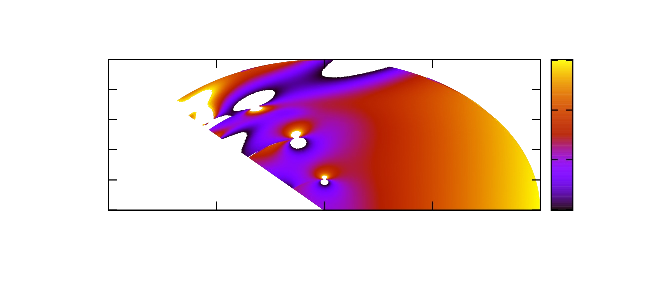
\includegraphics{monopole_anal_h_real}}%
    \gplfronttext
  \end{picture}%
\endgroup

        \caption{\em Real part of the function $M(z)$ (not $M(z)/z$,
          as on Fig. \ref{fig:2d_monopole_f}) for $\lambda = 0.5$. The
          function is even under conjugation: $\Re M(z) = \Re M(\bar
          z)$. The extended white regions correspond to
          out of range values.}
        \label{fig:cm_monopole_h_real}
      \end{center}
    \end{figure}

    \begin{figure}[!ht]
      \begin{center}
        % GNUPLOT: LaTeX picture with Postscript
\begingroup
  \makeatletter
  \providecommand\color[2][]{%
    \GenericError{(gnuplot) \space\space\space\@spaces}{%
      Package color not loaded in conjunction with
      terminal option `colourtext'%
    }{See the gnuplot documentation for explanation.%
    }{Either use 'blacktext' in gnuplot or load the package
      color.sty in LaTeX.}%
    \renewcommand\color[2][]{}%
  }%
  \providecommand\includegraphics[2][]{%
    \GenericError{(gnuplot) \space\space\space\@spaces}{%
      Package graphicx or graphics not loaded%
    }{See the gnuplot documentation for explanation.%
    }{The gnuplot epslatex terminal needs graphicx.sty or graphics.sty.}%
    \renewcommand\includegraphics[2][]{}%
  }%
  \providecommand\rotatebox[2]{#2}%
  \@ifundefined{ifGPcolor}{%
    \newif\ifGPcolor
    \GPcolortrue
  }{}%
  \@ifundefined{ifGPblacktext}{%
    \newif\ifGPblacktext
    \GPblacktexttrue
  }{}%
  % define a \g@addto@macro without @ in the name:
  \let\gplgaddtomacro\g@addto@macro
  % define empty templates for all commands taking text:
  \gdef\gplbacktext{}%
  \gdef\gplfronttext{}%
  \makeatother
  \ifGPblacktext
    % no textcolor at all
    \def\colorrgb#1{}%
    \def\colorgray#1{}%
  \else
    % gray or color?
    \ifGPcolor
      \def\colorrgb#1{\color[rgb]{#1}}%
      \def\colorgray#1{\color[gray]{#1}}%
      \expandafter\def\csname LTw\endcsname{\color{white}}%
      \expandafter\def\csname LTb\endcsname{\color{black}}%
      \expandafter\def\csname LTa\endcsname{\color{black}}%
      \expandafter\def\csname LT0\endcsname{\color[rgb]{1,0,0}}%
      \expandafter\def\csname LT1\endcsname{\color[rgb]{0,1,0}}%
      \expandafter\def\csname LT2\endcsname{\color[rgb]{0,0,1}}%
      \expandafter\def\csname LT3\endcsname{\color[rgb]{1,0,1}}%
      \expandafter\def\csname LT4\endcsname{\color[rgb]{0,1,1}}%
      \expandafter\def\csname LT5\endcsname{\color[rgb]{1,1,0}}%
      \expandafter\def\csname LT6\endcsname{\color[rgb]{0,0,0}}%
      \expandafter\def\csname LT7\endcsname{\color[rgb]{1,0.3,0}}%
      \expandafter\def\csname LT8\endcsname{\color[rgb]{0.5,0.5,0.5}}%
    \else
      % gray
      \def\colorrgb#1{\color{black}}%
      \def\colorgray#1{\color[gray]{#1}}%
      \expandafter\def\csname LTw\endcsname{\color{white}}%
      \expandafter\def\csname LTb\endcsname{\color{black}}%
      \expandafter\def\csname LTa\endcsname{\color{black}}%
      \expandafter\def\csname LT0\endcsname{\color{black}}%
      \expandafter\def\csname LT1\endcsname{\color{black}}%
      \expandafter\def\csname LT2\endcsname{\color{black}}%
      \expandafter\def\csname LT3\endcsname{\color{black}}%
      \expandafter\def\csname LT4\endcsname{\color{black}}%
      \expandafter\def\csname LT5\endcsname{\color{black}}%
      \expandafter\def\csname LT6\endcsname{\color{black}}%
      \expandafter\def\csname LT7\endcsname{\color{black}}%
      \expandafter\def\csname LT8\endcsname{\color{black}}%
    \fi
  \fi
  \setlength{\unitlength}{0.0500bp}%
  \begin{picture}(6236.00,2834.00)%
    \gplgaddtomacro\gplbacktext{%
    }%
    \gplgaddtomacro\gplfronttext{%
      \csname LTb\endcsname%
      \put(1046,517){\makebox(0,0){\strut{}-10}}%
      \put(2082,517){\makebox(0,0){\strut{}-5}}%
      \put(3118,517){\makebox(0,0){\strut{} 0}}%
      \put(4154,517){\makebox(0,0){\strut{} 5}}%
      \put(5190,517){\makebox(0,0){\strut{} 10}}%
      \put(3118,187){\makebox(0,0){\strut{}$x$}}%
      \put(874,803){\makebox(0,0)[r]{\strut{} 0}}%
      \put(874,1093){\makebox(0,0)[r]{\strut{} 2}}%
      \put(874,1383){\makebox(0,0)[r]{\strut{} 4}}%
      \put(874,1671){\makebox(0,0)[r]{\strut{} 6}}%
      \put(874,1961){\makebox(0,0)[r]{\strut{} 8}}%
      \put(874,2251){\makebox(0,0)[r]{\strut{} 10}}%
      \put(412,1527){\rotatebox{-270}{\makebox(0,0){\strut{}$y$}}}%
      \put(5633,811){\makebox(0,0)[l]{\strut{}-5}}%
      \put(5633,1288){\makebox(0,0)[l]{\strut{} 0}}%
      \put(5633,1764){\makebox(0,0)[l]{\strut{} 5}}%
      \put(5633,2241){\makebox(0,0)[l]{\strut{} 10}}%
    }%
    \gplbacktext
    \put(0,0){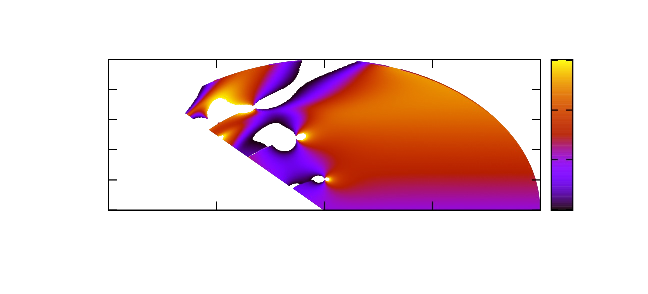
\includegraphics{monopole_anal_h_imag}}%
    \gplfronttext
  \end{picture}%
\endgroup

        \caption{\em Imaginary part of the function $M(z)$ for
          $\lambda = 0.5$. The function is odd under conjugation:
          $\Im M(z) = -\Im M(\bar z)$. The extended white regions correspond to
          out of range values.}
        \label{fig:cm_monopole_h_imag}
      \end{center}
    \end{figure}
  \end{subsection}
\end{section}

\begin{section}{Conclusion}
  We have been able, using our numerical procedure, to find a
  numerical analytic continuation for a vortex and the 't
  Hooft--Polyakov monopole in the Georgi--Glashow model. In both case,
  the solutions showed no singulary in the positive real half of the
  complex plane, at least in a radius $R=10$ around the
  origin. Obtaining the instanton with a Wick rotation of the soliton
  should therefore be possible.  There are still many leads to explore
  in order to close the subject. First of all, the actual
  implementation is difficult to generalize to an arbitrary, and its
  only purpose is as a proof of concept. In order to use it in a
  production environment, it should be rewritten to benefit from all
  the existing tools that already exist, and that are much more
  efficient.

  The convergence study of the Taylor series has been investigated
  for the vortex only. But the situation is different for the 't
  Hooft--Polyakov monopole.  The existance of a solution expressed in
  terms of elementary function in the BPS limit may bring some lights
  on the convergence properties of the series.

  A last feature provided by the numerical analytic continuation has
  still not been exploited. Using the freedom of the choice of the
  coordinate system, we could choose a polar coordinate system
  centered on a singularity, giving the possibility to obtain the a
  numerical solution on a closed path around a singularity. Such a
  numerical solution may allow a deeper inverstigation on the
  properties of the singularities.
  
  %At this point, I want to mention at least the following points:
  %\begin{itemize}
  %\item What have been done, concretely: Although numerical
  %  approximation of the solutions of the field equation have been
  %  known for a long time, it is still necessary to reproduce the
  %  result. A general mathematical framework has been developed, and
  %  given any differential system of equation we are able to compute
  %  numerically its analytic continuation to the complex plane, with
  %  an arbitrary system of coordinates. This may in particular be
  %  useful to investigate the properties of the singularities.
  % \item The difficulties? What were the difficulties? Most of them
  %  Where related to the numerical code, or to my working habits. I
  %  discovered that as long as writing code is not for pedagogical
  %  reasons, one should avoid at any price to reinvent the wheel. This
  %  introduce a lot of difficulties (which, in themselves are
  %  interesting, but that's not the point!), and many people
  %  accomplished the work many years ago, so why not benefit of their
  %  work?
  %
  %  Ah! Yes, we had this idea of finding the Laurent series of the
  %  solution around $0$, and find an approximation of the radius of
  %  convergence. It seem that we numerically observe singularities
  %  under the estimated radius of convergence. So it is still unclear
  %  why, and find where is the flaws. On my opinion, one should try
  %   the same approach with the monopole, since in the BPS limit we
  %   have a closed-form solution. 
  % \item What should be done now? There is much work to be done on the
  %   implementation of the method, in order to make it usable in
  %   production. In particular, it would be wise to use some
  %   well-tested, bug-free and efficient code which have proven
  %   robustness in various application. Such tool are often freely
  %   available in the form of Fortran routines.  An other thing which
  %   should be investigated is the possibility of changing the
  %   coordinate system during the integration, allowing to choose the
  %   path more freely. Finding a parametrization of a path is generally 
  %   an issue. Using successive well chosen coordinate system may
  %   solve it.
  % \item A word on the application as a part of any larger project, which
  %   I would be glad to head about.
  %\end{itemize}
  
\end{section}
